\section{System dynamics}
\label{sec:pipe_dynamics}

In this section the speed of dynamics for the test setup without the water tank is investigated.

%\subsection{One clamp push} % \label{app:...}
\subsection*{Test equipment:}
\begin{itemize}
\item The water distribution system at AAU.
\end{itemize}

\subsection*{Procedure:}
The following procedure was made for finding the time constant:
\begin{enumerate}
\item Disconnect the WT from the test setup.	
\item The initial setup of the system at time t=0 is chosen as, the valve opening at 0.7 for all consumer valves and the rotational speed of the pumps set to C2 = C16 = 3, C18 = 0.7, C25 = 4.2.
\item Reduce the rotational speed of C2 and C16 to 1.2 at time t=30.
\item Increase the rotational speed of C2 and C16 to 2.5 at time t=45.
\item Reduce the rotational speed of C2 and C16 to 1.5 at time t=60.
\item Increase the rotational speed of C2 and C16 to 3 at time t=75.
\end{enumerate}

\subsection*{Measuring data:}
The measurements data can be found on the attached storage under the path: \path{CD:/Data/system dynamics}.

\subsection*{Results:}

The step input given to the rotational speed of the two main pumps results in a change of differential pressure across the pumps. The measured differential pressure is shown in \figref{fig:Test_pipe_pumpdiff}. 

\begin{figure}[H]
% This file was created by matlab2tikz.
%
%The latest updates can be retrieved from
%  http://www.mathworks.com/matlabcentral/fileexchange/22022-matlab2tikz-matlab2tikz
%where you can also make suggestions and rate matlab2tikz.
%
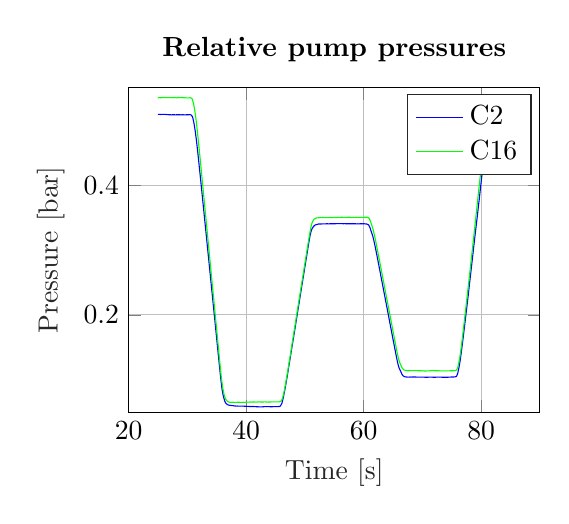
\begin{tikzpicture}

\begin{axis}[%
width=2.0556in,
height=1.62135in,
at={(1.011in,0.642in)},
scale only axis,
xmin=20,
xmax=90,
xlabel style={font=\color{white!15!black}},
xlabel={Time [s]},
ymin=0.05,
ymax=0.55,
ylabel style={font=\color{white!15!black}},
ylabel={Pressure [bar]},
axis background/.style={fill=white},
title style={font=\bfseries},
title={Relative pump pressures},
xmajorgrids,
ymajorgrids,
legend style={legend cell align=left, align=left, draw=white!15!black}
]
\addplot [color=blue]
  table[row sep=crcr]{%
24.95	0.509200879765406\\
25	0.509219208211154\\
25.05	0.509219208211154\\
25.1	0.50922531769307\\
25.15	0.509213098729237\\
25.2	0.509182551319657\\
25.25	0.509133675464329\\
25.3	0.509078690127085\\
25.35	0.509023704789841\\
25.4	0.508993157380261\\
25.45	0.509011485826009\\
25.5	0.509054252199421\\
25.55	0.509109237536665\\
25.6	0.509152003910077\\
25.65	0.509158113391993\\
25.7	0.509145894428161\\
25.75	0.509121456500497\\
25.8	0.509103128054749\\
25.85	0.509103128054749\\
25.9	0.509103128054749\\
25.95	0.509097018572833\\
26	0.509103128054749\\
26.05	0.509115347018582\\
26.1	0.50910312805475\\
26.15	0.509066471163254\\
26.2	0.509035923753673\\
26.25	0.509035923753673\\
26.3	0.509035923753673\\
26.35	0.508999266862176\\
26.4	0.508932062561101\\
26.45	0.508870967741941\\
26.5	0.508834310850444\\
26.55	0.508803763440864\\
26.6	0.508760997067452\\
26.65	0.50871823069404\\
26.7	0.50868768328446\\
26.75	0.508669354838712\\
26.8	0.508638807429132\\
26.85	0.508602150537635\\
26.9	0.508571603128055\\
26.95	0.508559384164223\\
27	0.508534946236559\\
27.05	0.508504398826979\\
27.1	0.508498289345063\\
27.15	0.508473851417399\\
27.2	0.508455522971651\\
27.25	0.508449413489735\\
27.3	0.508443304007819\\
27.35	0.508467741935483\\
27.4	0.508504398826979\\
27.45	0.508516617790811\\
27.5	0.508522727272727\\
27.55	0.508528836754643\\
27.6	0.50853494623656\\
27.65	0.508541055718476\\
27.7	0.50853494623656\\
27.75	0.50850439882698\\
27.8	0.508486070381233\\
27.85	0.508479960899317\\
27.9	0.508449413489737\\
27.95	0.508437194525905\\
28	0.508449413489737\\
28.05	0.508467741935485\\
28.1	0.508510508308897\\
28.15	0.508547165200393\\
28.2	0.508547165200393\\
28.25	0.508541055718477\\
28.3	0.508553274682309\\
28.35	0.508565493646141\\
28.4	0.508559384164225\\
28.45	0.508547165200392\\
28.5	0.508553274682309\\
28.55	0.508559384164225\\
28.6	0.508565493646141\\
28.65	0.508553274682309\\
28.7	0.508534946236561\\
28.75	0.508516617790813\\
28.8	0.508473851417401\\
28.85	0.508449413489737\\
28.9	0.508449413489737\\
28.95	0.508467741935485\\
29	0.508479960899317\\
29.05	0.508486070381233\\
29.1	0.508492179863149\\
29.15	0.508498289345065\\
29.2	0.508504398826982\\
29.25	0.508516617790814\\
29.3	0.508510508308898\\
29.35	0.508467741935486\\
29.4	0.508406647116326\\
29.45	0.508363880742914\\
29.5	0.508345552297166\\
29.55	0.508351661779082\\
29.6	0.508388318670579\\
29.65	0.508424975562075\\
29.7	0.508455522971655\\
29.75	0.50847996089932\\
29.8	0.508492179863152\\
29.85	0.508498289345068\\
29.9	0.508522727272732\\
29.95	0.508553274682311\\
30	0.508565493646143\\
30.05	0.508565493646143\\
30.1	0.508565493646143\\
30.15	0.508583822091891\\
30.2	0.508608260019555\\
30.25	0.508626588465303\\
30.3	0.508657135874883\\
30.35	0.508693792766379\\
30.4	0.508712121212127\\
30.45	0.508657135874883\\
30.5	0.508565493646143\\
30.55	0.508467741935488\\
30.6	0.508345552297169\\
30.65	0.507991202346044\\
30.7	0.50741080156403\\
30.75	0.506824291300101\\
30.8	0.506219452590424\\
30.85	0.505620723362662\\
30.9	0.504307184750737\\
30.95	0.502291055718479\\
31	0.500299364613884\\
31.05	0.498289345063542\\
31.1	0.495912756598244\\
31.15	0.493187927663738\\
31.2	0.490432551319652\\
31.25	0.487652737047903\\
31.3	0.484891251221901\\
31.35	0.481750977517112\\
31.4	0.478250244379282\\
31.45	0.474773949169116\\
31.5	0.471291544477035\\
31.55	0.467515884652988\\
31.6	0.463453079178892\\
31.65	0.45938416422288\\
31.7	0.455296920821121\\
31.75	0.451215786901277\\
31.8	0.44707966764419\\
31.85	0.442851906158364\\
31.9	0.438599706744875\\
31.95	0.434323069403721\\
32	0.429991446725324\\
32.05	0.425623167155432\\
32.1	0.421242668621708\\
32.15	0.4168682795699\\
32.2	0.412487781036175\\
32.25	0.408076735092871\\
32.3	0.403647360703819\\
32.35	0.399199657869019\\
32.4	0.394745845552303\\
32.45	0.390292033235588\\
32.5	0.385813782991208\\
32.55	0.381317204301081\\
32.6	0.376851173020533\\
32.65	0.37240957966765\\
32.7	0.367943548387103\\
32.75	0.363477517106555\\
32.8	0.359005376344091\\
32.85	0.354502688172048\\
32.9	0.350012218963837\\
32.95	0.345564516129037\\
33	0.341122922776154\\
33.05	0.336669110459438\\
33.1	0.332209188660807\\
33.15	0.327724828934512\\
33.2	0.3232343597263\\
33.25	0.318750000000005\\
33.3	0.314259530791794\\
33.35	0.309744623655919\\
33.4	0.30523582600196\\
33.45	0.300745356793749\\
33.5	0.296236559139791\\
33.55	0.29174608993158\\
33.6	0.287255620723369\\
33.65	0.282759042033242\\
33.7	0.278274682306947\\
33.75	0.273802541544483\\
33.8	0.269342619745853\\
33.85	0.264846041055726\\
33.9	0.260325024437935\\
33.95	0.255791788856312\\
34	0.251282991202353\\
34.05	0.246792521994142\\
34.1	0.242302052785931\\
34.15	0.23781158357772\\
34.2	0.233315004887593\\
34.25	0.22881231671555\\
34.3	0.224315738025424\\
34.35	0.219849706744877\\
34.4	0.215395894428162\\
34.45	0.210917644183782\\
34.5	0.206433284457487\\
34.55	0.201967253176939\\
34.6	0.197470674486812\\
34.65	0.192961876832853\\
34.7	0.188465298142726\\
34.75	0.183956500488767\\
34.8	0.179441593352892\\
34.85	0.174932795698933\\
34.9	0.170411779081142\\
34.95	0.165878543499519\\
35	0.16136974584556\\
35.05	0.156873167155433\\
35.1	0.152376588465306\\
35.15	0.147886119257095\\
35.2	0.1434017595308\\
35.25	0.138941837732169\\
35.3	0.134488025415454\\
35.35	0.130028103616822\\
35.4	0.125574291300107\\
35.45	0.121151026392971\\
35.5	0.116715542522004\\
35.55	0.112267839687205\\
35.6	0.107850684261986\\
35.65	0.103696236559151\\
35.7	0.0998044965787013\\
35.75	0.0959127565982517\\
35.8	0.092021016617802\\
35.85	0.0881170576735205\\
35.9	0.0849279081134032\\
35.95	0.0824657869012821\\
36	0.0799608993157495\\
36.05	0.0774437927663851\\
36.1	0.0753299120234722\\
36.15	0.0736009286412632\\
36.2	0.0718963831867178\\
36.25	0.0702040566960044\\
36.3	0.068505620723375\\
36.35	0.0671981915933653\\
36.4	0.0662573313783117\\
36.45	0.0652798142717625\\
36.5	0.0643022971652133\\
36.55	0.063624144672545\\
36.6	0.0632270283480096\\
36.65	0.0628421309873062\\
36.7	0.0624877810361824\\
36.75	0.0621212121212267\\
36.8	0.0617974095796825\\
36.85	0.0615591397849613\\
36.9	0.0613391984359879\\
36.95	0.0611192570870145\\
37	0.0609481915933685\\
37.05	0.0608382209188818\\
37.1	0.060734359726311\\
37.15	0.0606182795699084\\
37.2	0.0605144183773376\\
37.25	0.0604533235581783\\
37.3	0.060398338220935\\
37.35	0.0603433528836916\\
37.4	0.0602883675464483\\
37.45	0.060227272727289\\
37.5	0.0601906158357934\\
37.55	0.0601783968719616\\
37.6	0.060141739980466\\
37.65	0.0600745356793908\\
37.7	0.0600256598240634\\
37.75	0.0599645650049041\\
37.8	0.059891251221913\\
37.85	0.0598362658846696\\
37.9	0.0597812805474263\\
37.95	0.0597018572825192\\
38	0.0596224340176121\\
38.05	0.0595613391984529\\
38.1	0.0595063538612095\\
38.15	0.0594696969697139\\
38.2	0.0594513685239662\\
38.25	0.0594208211143865\\
38.3	0.059378054740975\\
38.35	0.0593719452590591\\
38.4	0.059378054740975\\
38.45	0.0593841642228909\\
38.5	0.0593963831867228\\
38.55	0.0593841642228909\\
38.6	0.0593536168133113\\
38.65	0.0593230694037317\\
38.7	0.0593108504398998\\
38.75	0.0593047409579839\\
38.8	0.0592864125122361\\
38.85	0.0592741935484042\\
38.9	0.0592741935484042\\
38.95	0.0592864125122361\\
39	0.059298631476068\\
39.05	0.0593108504398998\\
39.1	0.0593230694037317\\
39.15	0.0593413978494794\\
39.2	0.0593413978494794\\
39.25	0.0593352883675635\\
39.3	0.0593413978494794\\
39.35	0.0593230694037317\\
39.4	0.059298631476068\\
39.45	0.0592741935484042\\
39.5	0.0592375366569087\\
39.55	0.0592008797654131\\
39.6	0.0591703323558335\\
39.65	0.0591397849462538\\
39.7	0.0591092375366742\\
39.75	0.0590909090909264\\
39.8	0.0590725806451786\\
39.85	0.0590359237536831\\
39.9	0.0590053763441034\\
39.95	0.0589931573802716\\
40	0.0590053763441034\\
40.05	0.0590175953079353\\
40.1	0.0590114858260193\\
40.15	0.0589931573802716\\
40.2	0.0589626099706919\\
40.25	0.0589320625611123\\
40.3	0.0589015151515326\\
40.35	0.0588465298142893\\
40.4	0.0587915444770459\\
40.45	0.0587609970674663\\
40.5	0.0587609970674663\\
40.55	0.0587671065493822\\
40.6	0.0587548875855504\\
40.65	0.0587304496578867\\
40.7	0.0586876832844752\\
40.75	0.0586510263929796\\
40.8	0.0586326979472318\\
40.85	0.0586388074291477\\
40.9	0.0586265884653159\\
40.95	0.0585899315738203\\
41	0.0585960410557362\\
41.05	0.0586265884653159\\
41.1	0.0586449169110637\\
41.15	0.0586510263929796\\
41.2	0.0586388074291477\\
41.25	0.0586265884653159\\
41.3	0.058614369501484\\
41.35	0.0586021505376522\\
41.4	0.0585899315738203\\
41.45	0.0585838220919044\\
41.5	0.0585838220919044\\
41.55	0.0585471652004088\\
41.6	0.0584982893450814\\
41.65	0.058449413489754\\
41.7	0.0583822091886788\\
41.75	0.0583150048876036\\
41.8	0.0582844574780239\\
41.85	0.0582844574780239\\
41.9	0.058278347996108\\
41.95	0.0582661290322761\\
42	0.0582600195503602\\
42.05	0.0582478005865283\\
42.1	0.0582111436950328\\
42.15	0.0581805962854531\\
42.2	0.0581561583577894\\
42.25	0.0581317204301257\\
42.3	0.0581256109482098\\
42.35	0.0581195014662939\\
42.4	0.0581195014662939\\
42.45	0.0581317204301257\\
42.5	0.0581500488758735\\
42.55	0.0581622678397054\\
42.6	0.0581622678397054\\
42.65	0.0581622678397054\\
42.7	0.0581744868035372\\
42.75	0.0581989247312009\\
42.8	0.0582233626588646\\
42.85	0.0582600195503602\\
42.9	0.0583027859237717\\
42.95	0.0583455522971832\\
43	0.0583822091886788\\
43.05	0.0584188660801743\\
43.1	0.058449413489754\\
43.15	0.0584860703812495\\
43.2	0.0585105083089132\\
43.25	0.0585166177908292\\
43.3	0.0585227272727451\\
43.35	0.0584982893450814\\
43.4	0.0584799608993336\\
43.45	0.0584799608993336\\
43.5	0.0584677419355017\\
43.55	0.058449413489754\\
43.6	0.0584555229716699\\
43.65	0.0584616324535858\\
43.7	0.058449413489754\\
43.75	0.0584371945259221\\
43.8	0.0584371945259221\\
43.85	0.058443304007838\\
43.9	0.058449413489754\\
43.95	0.058449413489754\\
44	0.0584188660801743\\
44.05	0.0583883186705947\\
44.1	0.0583760997067628\\
44.15	0.058357771261015\\
44.2	0.058357771261015\\
44.25	0.058357771261015\\
44.3	0.0583455522971832\\
44.35	0.0583516617790991\\
44.4	0.058357771261015\\
44.45	0.0583760997067628\\
44.5	0.0584066471163425\\
44.55	0.0584066471163425\\
44.6	0.0584188660801743\\
44.65	0.0584555229716699\\
44.7	0.0584982893450814\\
44.75	0.0585471652004088\\
44.8	0.0585654936461566\\
44.85	0.0585838220919044\\
44.9	0.0586021505376522\\
44.95	0.0585960410557362\\
45	0.0585716031280725\\
45.05	0.0585593841642407\\
45.1	0.0585654936461566\\
45.15	0.0585777126099885\\
45.2	0.0586021505376522\\
45.25	0.058614369501484\\
45.3	0.0586082600195681\\
45.35	0.0586082600195681\\
45.4	0.0586082600195681\\
45.45	0.058614369501484\\
45.5	0.0586204789833999\\
45.55	0.0586265884653159\\
45.6	0.0586449169110637\\
45.65	0.0587426686217185\\
45.7	0.0589137341153645\\
45.75	0.0590909090909264\\
45.8	0.0592558651026565\\
45.85	0.0597446236559311\\
45.9	0.060575513196498\\
45.95	0.0614125122189808\\
46	0.0622617302052955\\
46.05	0.0630987292277784\\
46.1	0.0644000488758721\\
46.15	0.0661595796676608\\
46.2	0.0679435483871131\\
46.25	0.0697336265884815\\
46.3	0.071700879765412\\
46.35	0.0738697458455686\\
46.4	0.076056940371473\\
46.45	0.0782563538612092\\
46.5	0.0804374389051976\\
46.55	0.0827651515151683\\
46.6	0.0852333822092053\\
46.65	0.0876955034213264\\
46.7	0.0901759530791953\\
46.75	0.0927663734115509\\
46.8	0.0954484359726454\\
46.85	0.0981060606060762\\
46.9	0.100763685239507\\
46.95	0.103439638318686\\
47	0.106133919843612\\
47.05	0.108852639296202\\
47.1	0.111608015640288\\
47.15	0.114375610948205\\
47.2	0.117118768328459\\
47.25	0.119837487781049\\
47.3	0.122568426197471\\
47.35	0.125317693059641\\
47.4	0.128054740957979\\
47.45	0.130828445747812\\
47.5	0.133632697947225\\
47.55	0.136436950146638\\
47.6	0.139247311827967\\
47.65	0.142063782991212\\
47.7	0.144874144672541\\
47.75	0.147672287390038\\
47.8	0.150470430107535\\
47.85	0.153250244379285\\
47.9	0.156023949169118\\
47.95	0.158791544477036\\
48	0.161565249266869\\
48.05	0.164345063538618\\
48.1	0.167112658846536\\
48.15	0.169898582600201\\
48.2	0.172715053763446\\
48.25	0.175543743890523\\
48.3	0.178360215053768\\
48.35	0.181170576735097\\
48.4	0.18397482893451\\
48.45	0.186779081133923\\
48.5	0.189601661779084\\
48.55	0.192430351906161\\
48.6	0.195252932551321\\
48.65	0.198075513196482\\
48.7	0.200904203323559\\
48.75	0.203732893450636\\
48.8	0.206555474095797\\
48.85	0.209384164222874\\
48.9	0.21221285434995\\
48.95	0.215047653958943\\
49	0.217894672531768\\
49.05	0.220717253176928\\
49.1	0.223521505376342\\
49.15	0.226313538611923\\
49.2	0.229105571847504\\
49.25	0.231934261974581\\
49.3	0.234762952101658\\
49.35	0.237585532746818\\
49.4	0.240420332355811\\
49.45	0.24323069403714\\
49.5	0.246022727272721\\
49.55	0.248820869990218\\
49.6	0.251619012707716\\
49.65	0.254429374389045\\
49.7	0.257233626588458\\
49.75	0.260013440860207\\
49.8	0.262805474095788\\
49.85	0.265591397849454\\
49.9	0.268377321603119\\
49.95	0.271187683284448\\
50	0.274004154447693\\
50.05	0.276820625610938\\
50.1	0.279630987292267\\
50.15	0.282441348973596\\
50.2	0.285251710654925\\
50.25	0.288062072336254\\
50.3	0.290872434017583\\
50.35	0.293701124144659\\
50.4	0.296542033235568\\
50.45	0.299364613880729\\
50.5	0.302193304007806\\
50.55	0.305015884652967\\
50.6	0.307814027370464\\
50.65	0.31053885630497\\
50.7	0.313190371456485\\
50.75	0.315860215053747\\
50.8	0.318542277614842\\
50.85	0.320863880742896\\
50.9	0.322843352883658\\
50.95	0.324804496578673\\
51	0.326747311827939\\
51.05	0.32868401759529\\
51.1	0.330168621700861\\
51.15	0.331219452590402\\
51.2	0.332239736070362\\
51.25	0.333260019550323\\
51.3	0.334103128054721\\
51.35	0.334738514173978\\
51.4	0.335355571847487\\
51.45	0.335966520039079\\
51.5	0.33659579667642\\
51.55	0.337102883675442\\
51.6	0.337487781036145\\
51.65	0.337866568914933\\
51.7	0.33824535679372\\
51.75	0.338526392961853\\
51.8	0.338685239491667\\
51.85	0.338844086021481\\
51.9	0.339021260997043\\
51.95	0.339204545454521\\
52	0.339363391984335\\
52.05	0.33949169110457\\
52.1	0.339589442815225\\
52.15	0.339681085043964\\
52.2	0.339797165200366\\
52.25	0.339907135874853\\
52.3	0.339992668621676\\
52.35	0.340059872922751\\
52.4	0.34012096774191\\
52.45	0.340145405669574\\
52.5	0.340133186705742\\
52.55	0.340133186705742\\
52.6	0.340145405669574\\
52.65	0.340163734115322\\
52.7	0.340175953079154\\
52.75	0.340175953079154\\
52.8	0.340169843597238\\
52.85	0.340194281524902\\
52.9	0.340237047898313\\
52.95	0.340273704789809\\
53	0.340292033235556\\
53.05	0.340292033235556\\
53.1	0.340304252199388\\
53.15	0.340292033235556\\
53.2	0.340267595307893\\
53.25	0.340255376344061\\
53.3	0.340261485825977\\
53.35	0.34028592375364\\
53.4	0.340298142717472\\
53.45	0.340310361681304\\
53.5	0.340334799608968\\
53.55	0.340359237536632\\
53.6	0.340383675464295\\
53.65	0.340420332355791\\
53.7	0.34045087976537\\
53.75	0.340475317693034\\
53.8	0.340475317693034\\
53.85	0.340444770283455\\
53.9	0.340414222873875\\
53.95	0.340365347018547\\
54	0.340322580645136\\
54.05	0.340334799608968\\
54.1	0.340371456500463\\
54.15	0.340395894428127\\
54.2	0.340414222873875\\
54.25	0.340426441837707\\
54.3	0.340463098729202\\
54.35	0.340487536656866\\
54.4	0.340487536656866\\
54.45	0.340518084066446\\
54.5	0.340524193548362\\
54.55	0.34051197458453\\
54.6	0.340518084066446\\
54.65	0.340499755620698\\
54.7	0.340487536656866\\
54.75	0.340493646138782\\
54.8	0.34051197458453\\
54.85	0.340536412512193\\
54.9	0.340548631476025\\
54.95	0.340548631476025\\
55	0.340530303030278\\
55.05	0.340518084066446\\
55.1	0.34051197458453\\
55.15	0.34051197458453\\
55.2	0.340536412512193\\
55.25	0.340585288367521\\
55.3	0.34064638318668\\
55.35	0.34067693059626\\
55.4	0.340689149560092\\
55.45	0.340707478005839\\
55.5	0.340713587487755\\
55.55	0.340719696969671\\
55.6	0.340750244379251\\
55.65	0.340768572824999\\
55.7	0.340774682306915\\
55.75	0.340774682306915\\
55.8	0.340756353861167\\
55.85	0.340744134897335\\
55.9	0.340744134897335\\
55.95	0.340762463343083\\
56	0.340762463343083\\
56.05	0.340756353861167\\
56.1	0.340750244379251\\
56.15	0.340713587487755\\
56.2	0.340683040078176\\
56.25	0.340664711632428\\
56.3	0.340634164222848\\
56.35	0.340597507331353\\
56.4	0.340579178885605\\
56.45	0.340573069403689\\
56.5	0.340560850439857\\
56.55	0.340548631476025\\
56.6	0.340560850439857\\
56.65	0.340597507331353\\
56.7	0.340609726295185\\
56.75	0.340591397849437\\
56.8	0.340579178885605\\
56.85	0.340579178885605\\
56.9	0.340560850439857\\
56.95	0.340536412512193\\
57	0.340518084066446\\
57.05	0.340493646138782\\
57.1	0.340487536656866\\
57.15	0.340493646138782\\
57.2	0.340487536656866\\
57.25	0.340475317693034\\
57.3	0.340463098729202\\
57.35	0.340456989247286\\
57.4	0.340456989247286\\
57.45	0.340475317693034\\
57.5	0.340499755620698\\
57.55	0.340505865102614\\
57.6	0.340518084066446\\
57.65	0.340518084066446\\
57.7	0.340518084066446\\
57.75	0.340518084066446\\
57.8	0.340505865102614\\
57.85	0.340493646138782\\
57.9	0.340493646138782\\
57.95	0.340505865102614\\
58	0.340524193548362\\
58.05	0.340548631476025\\
58.1	0.340554740957941\\
58.15	0.340542521994109\\
58.2	0.340518084066446\\
58.25	0.340493646138782\\
58.3	0.340469208211118\\
58.35	0.340456989247286\\
58.4	0.340469208211118\\
58.45	0.340475317693034\\
58.5	0.340469208211118\\
58.55	0.340469208211118\\
58.6	0.340456989247286\\
58.65	0.340426441837707\\
58.7	0.340389784946211\\
58.75	0.340353128054716\\
58.8	0.3403470185728\\
58.85	0.340365347018547\\
58.9	0.340377565982379\\
58.95	0.340402003910043\\
59	0.340426441837707\\
59.05	0.340414222873875\\
59.1	0.340395894428127\\
59.15	0.340395894428127\\
59.2	0.340402003910043\\
59.25	0.340402003910043\\
59.3	0.340395894428127\\
59.35	0.340414222873875\\
59.4	0.340426441837707\\
59.45	0.340408113391959\\
59.5	0.340408113391959\\
59.55	0.340414222873875\\
59.6	0.340414222873875\\
59.65	0.340420332355791\\
59.7	0.340408113391959\\
59.75	0.340402003910043\\
59.8	0.340408113391959\\
59.85	0.340426441837707\\
59.9	0.340456989247286\\
59.95	0.340475317693034\\
60	0.340487536656866\\
60.05	0.340475317693034\\
60.1	0.34045087976537\\
60.15	0.340414222873875\\
60.2	0.340359237536632\\
60.25	0.340298142717472\\
60.3	0.340230938416397\\
60.35	0.340188172042986\\
60.4	0.340145405669574\\
60.45	0.340090420332331\\
60.5	0.340047653958919\\
60.55	0.340010997067424\\
60.6	0.339870478983357\\
60.65	0.339662756598216\\
60.7	0.339479472140738\\
60.75	0.339271749755596\\
60.8	0.339076246334287\\
60.85	0.338587487781012\\
60.9	0.337774926686194\\
60.95	0.336950146627544\\
61	0.336137585532725\\
61.05	0.335282258064495\\
61.1	0.334084799608973\\
61.15	0.332612414467233\\
61.2	0.331133919843577\\
61.25	0.329624877810341\\
61.3	0.328219696969676\\
61.35	0.32693670576733\\
61.4	0.3256598240469\\
61.45	0.324370723362637\\
61.5	0.323063294232627\\
61.55	0.321535923753644\\
61.6	0.319764173998023\\
61.65	0.317967986314739\\
61.7	0.316184017595287\\
61.75	0.31424120234602\\
61.8	0.31213954056694\\
61.85	0.310031769305943\\
61.9	0.307923998044947\\
61.95	0.305828445747782\\
62	0.303647360703794\\
62.05	0.301386852394899\\
62.1	0.299120234604089\\
62.15	0.296841397849446\\
62.2	0.294544232649056\\
62.25	0.292234848484834\\
62.3	0.289925464320611\\
62.35	0.287628299120221\\
62.4	0.285325024437915\\
62.45	0.282991202346029\\
62.5	0.280645161290311\\
62.55	0.278293010752677\\
62.6	0.275934750733128\\
62.65	0.273570381231662\\
62.7	0.271193792766365\\
62.75	0.268829423264899\\
62.8	0.266489491691097\\
62.85	0.264131231671548\\
62.9	0.261736314760503\\
62.95	0.259353616813289\\
63	0.256983137829908\\
63.05	0.254600439882694\\
63.1	0.252242179863145\\
63.15	0.249908357771259\\
63.2	0.247574535679373\\
63.25	0.245234604105571\\
63.3	0.242900782013685\\
63.35	0.240548631476052\\
63.4	0.238172043010754\\
63.45	0.235801564027373\\
63.5	0.233431085043991\\
63.55	0.231066715542526\\
63.6	0.228708455522976\\
63.65	0.226350195503427\\
63.7	0.223991935483877\\
63.75	0.221639784946243\\
63.8	0.219287634408609\\
63.85	0.216935483870976\\
63.9	0.214607771261006\\
63.95	0.212280058651036\\
64	0.209934017595318\\
64.05	0.207575757575768\\
64.1	0.205186950146639\\
64.15	0.202804252199426\\
64.2	0.20043988269796\\
64.25	0.198057184750747\\
64.3	0.195643939393954\\
64.35	0.193224584555245\\
64.4	0.190817448680368\\
64.45	0.188428641251239\\
64.5	0.186064271749773\\
64.55	0.183724340175971\\
64.6	0.181372189638338\\
64.65	0.179007820136872\\
64.7	0.17666788856307\\
64.75	0.174309628543521\\
64.8	0.171926930596307\\
64.85	0.16955034213101\\
64.9	0.167173753665713\\
64.95	0.164803274682331\\
65	0.162451124144697\\
65.05	0.160117302052812\\
65.1	0.157807917888589\\
65.15	0.155504643206283\\
65.2	0.153164711632481\\
65.25	0.150818670576763\\
65.3	0.148484848484878\\
65.35	0.146126588465328\\
65.4	0.14378054740961\\
65.45	0.141458944281556\\
65.5	0.139106793743922\\
65.55	0.136754643206289\\
65.6	0.134518572825058\\
65.65	0.132361925708734\\
65.7	0.130180840664746\\
65.75	0.127999755620758\\
65.8	0.125830889540602\\
65.85	0.123973607038159\\
65.9	0.12244012707726\\
65.95	0.12090664711636\\
66	0.119367057673545\\
66.05	0.117870234604141\\
66.1	0.116691104594366\\
66.15	0.115829667644221\\
66.2	0.114980449657907\\
66.25	0.114131231671593\\
66.3	0.113184261974624\\
66.35	0.112115102639336\\
66.4	0.111052052785965\\
66.45	0.109982893450677\\
66.5	0.108907624633474\\
66.55	0.108046187683328\\
66.6	0.107416911045988\\
66.65	0.106818181818227\\
66.7	0.10621334310855\\
66.75	0.105779569892519\\
66.8	0.105529081133966\\
66.85	0.105266373411581\\
66.9	0.105003665689196\\
66.95	0.104753176930643\\
67	0.104582111436997\\
67.05	0.104484359726342\\
67.1	0.104392717497603\\
67.15	0.10430718475078\\
67.2	0.104246089931621\\
67.25	0.104221652003957\\
67.3	0.104197214076294\\
67.35	0.104148338220966\\
67.4	0.104111681329471\\
67.45	0.104093352883723\\
67.5	0.104062805474143\\
67.55	0.10403836754648\\
67.6	0.104013929618816\\
67.65	0.104013929618816\\
67.7	0.104032258064564\\
67.75	0.104062805474143\\
67.8	0.104087243401807\\
67.85	0.104105571847555\\
67.9	0.104130009775218\\
67.95	0.104123900293303\\
68	0.104093352883723\\
68.05	0.104075024437975\\
68.1	0.104081133919891\\
68.15	0.104099462365639\\
68.2	0.104117790811387\\
68.25	0.104117790811387\\
68.3	0.104111681329471\\
68.35	0.104123900293303\\
68.4	0.104154447702882\\
68.45	0.104160557184798\\
68.5	0.104160557184798\\
68.55	0.104166666666714\\
68.6	0.104184995112462\\
68.65	0.10420332355821\\
68.7	0.10420332355821\\
68.75	0.10420332355821\\
68.8	0.104197214076294\\
68.85	0.10417277614863\\
68.9	0.104123900293303\\
68.95	0.104099462365639\\
69	0.104099462365639\\
69.05	0.104087243401807\\
69.1	0.104081133919891\\
69.15	0.104075024437975\\
69.2	0.104062805474143\\
69.25	0.104062805474143\\
69.3	0.104068914956059\\
69.35	0.104062805474143\\
69.4	0.104056695992227\\
69.45	0.104050586510311\\
69.5	0.104044477028395\\
69.55	0.10403836754648\\
69.6	0.10403836754648\\
69.65	0.104050586510311\\
69.7	0.104026148582648\\
69.75	0.1040078201369\\
69.8	0.104013929618816\\
69.85	0.103995601173068\\
69.9	0.103965053763488\\
69.95	0.103965053763488\\
70	0.10397727272732\\
70.05	0.103958944281572\\
70.1	0.103934506353909\\
70.15	0.103916177908161\\
70.2	0.103916177908161\\
70.25	0.103903958944329\\
70.3	0.103891739980497\\
70.35	0.103897849462413\\
70.4	0.103879521016665\\
70.45	0.10384286412517\\
70.5	0.103836754643254\\
70.55	0.103848973607086\\
70.6	0.10384286412517\\
70.65	0.103830645161338\\
70.7	0.103836754643254\\
70.75	0.10384286412517\\
70.8	0.103824535679422\\
70.85	0.103818426197506\\
70.9	0.103830645161338\\
70.95	0.103861192570918\\
71	0.103897849462413\\
71.05	0.103910068426245\\
71.1	0.103928396871993\\
71.15	0.103940615835825\\
71.2	0.103940615835825\\
71.25	0.103940615835825\\
71.3	0.103940615835825\\
71.35	0.103952834799657\\
71.4	0.103934506353909\\
71.45	0.103916177908161\\
71.5	0.103934506353909\\
71.55	0.103952834799657\\
71.6	0.103940615835825\\
71.65	0.103916177908161\\
71.7	0.103903958944329\\
71.75	0.103891739980497\\
71.8	0.103867302052834\\
71.85	0.103861192570918\\
71.9	0.103873411534749\\
71.95	0.103879521016665\\
72	0.103879521016665\\
72.05	0.103873411534749\\
72.1	0.103879521016665\\
72.15	0.103879521016665\\
72.2	0.103873411534749\\
72.25	0.103873411534749\\
72.3	0.103879521016665\\
72.35	0.103897849462413\\
72.4	0.103903958944329\\
72.45	0.103897849462413\\
72.5	0.103903958944329\\
72.55	0.103910068426245\\
72.6	0.103922287390077\\
72.65	0.103928396871993\\
72.7	0.103922287390077\\
72.75	0.103910068426245\\
72.8	0.103910068426245\\
72.85	0.103934506353909\\
72.9	0.103952834799657\\
72.95	0.103952834799657\\
73	0.103958944281572\\
73.05	0.103971163245404\\
73.1	0.103952834799657\\
73.15	0.103916177908161\\
73.2	0.103897849462413\\
73.25	0.103903958944329\\
73.3	0.103885630498581\\
73.35	0.103855083089002\\
73.4	0.103830645161338\\
73.45	0.103806207233674\\
73.5	0.103787878787927\\
73.55	0.103781769306011\\
73.6	0.103769550342179\\
73.65	0.103751221896431\\
73.7	0.103739002932599\\
73.75	0.103720674486851\\
73.8	0.103720674486851\\
73.85	0.103739002932599\\
73.9	0.103745112414515\\
73.95	0.103708455523019\\
74	0.103696236559188\\
74.05	0.103726783968767\\
74.1	0.103775659824095\\
74.15	0.103818426197506\\
74.2	0.103848973607086\\
74.25	0.103867302052834\\
74.3	0.103879521016665\\
74.35	0.103885630498581\\
74.4	0.103879521016665\\
74.45	0.103891739980497\\
74.5	0.103903958944329\\
74.55	0.103916177908161\\
74.6	0.103934506353909\\
74.65	0.103946725317741\\
74.7	0.10397727272732\\
74.75	0.1040078201369\\
74.8	0.10403836754648\\
74.85	0.104087243401807\\
74.9	0.104130009775218\\
74.95	0.104136119257134\\
75	0.104117790811387\\
75.05	0.104130009775218\\
75.1	0.104130009775218\\
75.15	0.104117790811387\\
75.2	0.104136119257134\\
75.25	0.10417277614863\\
75.3	0.10420332355821\\
75.35	0.104221652003957\\
75.4	0.104258308895453\\
75.45	0.104301075268864\\
75.5	0.104319403714612\\
75.55	0.104331622678444\\
75.6	0.104423264907183\\
75.65	0.104612658846577\\
75.7	0.104808162267886\\
75.75	0.10499755620728\\
75.8	0.105186950146674\\
75.85	0.105858993157426\\
75.9	0.107019794721452\\
75.95	0.108186705767395\\
76	0.109353616813337\\
76.05	0.111009286412554\\
76.1	0.113141495601214\\
76.15	0.115255376344127\\
76.2	0.117375366568955\\
76.25	0.119495356793784\\
76.3	0.121969696969736\\
76.35	0.124804496578728\\
76.4	0.127663734115384\\
76.45	0.130541300097787\\
76.5	0.133657135874913\\
76.55	0.137017350928676\\
76.6	0.140389784946271\\
76.65	0.14375610948195\\
76.7	0.147110215053797\\
76.75	0.150580400782047\\
76.8	0.1541666666667\\
76.85	0.157752932551352\\
76.9	0.161339198436005\\
76.95	0.164986559139817\\
77	0.168737781036199\\
77.05	0.172519550342162\\
77.1	0.176270772238544\\
77.15	0.180021994134927\\
77.2	0.183797653958973\\
77.25	0.187585532746851\\
77.3	0.191361192570898\\
77.35	0.195124633431112\\
77.4	0.19891251221899\\
77.45	0.202706500488785\\
77.5	0.206488269794747\\
77.55	0.210276148582625\\
77.6	0.214070136852419\\
77.65	0.217906891495625\\
77.7	0.221786412512242\\
77.75	0.225665933528859\\
77.8	0.229527126099728\\
77.85	0.233443304007841\\
77.9	0.237463343108524\\
77.95	0.241507820136872\\
78	0.245540078201387\\
78.05	0.249572336265902\\
78.1	0.253561827957006\\
78.15	0.257514662756614\\
78.2	0.261467497556222\\
78.25	0.265395894428167\\
78.3	0.269342619745859\\
78.35	0.273301564027383\\
78.4	0.277260508308908\\
78.45	0.281231671554264\\
78.5	0.285184506353872\\
78.55	0.289149560117312\\
78.6	0.293163489736079\\
78.65	0.297207966764427\\
78.7	0.301270772238522\\
78.75	0.305333577712616\\
78.8	0.309304740957973\\
78.85	0.313202590420337\\
78.9	0.31711876832845\\
78.95	0.321041055718479\\
79	0.324902248289348\\
79.05	0.328732893450638\\
79.1	0.332551319648096\\
79.15	0.336363636363637\\
79.2	0.340175953079179\\
79.25	0.344000488758553\\
79.3	0.347837243401759\\
79.35	0.351698435972628\\
79.4	0.355590175953077\\
79.45	0.359543010752685\\
79.5	0.3635752688172\\
79.55	0.367613636363632\\
79.6	0.371645894428147\\
79.65	0.375684261974578\\
79.7	0.379722629521009\\
79.75	0.383754887585525\\
79.8	0.387768817204292\\
79.85	0.391776637341144\\
79.9	0.395802785923743\\
79.95	0.399841153470175\\
80	0.403903958944269\\
80.05	0.407960654936449\\
80.1	0.412017350928628\\
80.15	0.416061827956975\\
80.2	0.420075757575742\\
80.25	0.42408968719451\\
80.3	0.428097507331361\\
80.35	0.432117546432045\\
80.4	0.43614980449656\\
80.45	0.440169843597243\\
80.5	0.444183773216011\\
80.55	0.448191593352863\\
80.6	0.452144428152471\\
80.65	0.456017839687172\\
80.7	0.459891251221873\\
80.75	0.463782991202322\\
80.8	0.467668621700855\\
80.85	0.471047165200366\\
80.9	0.473912512218939\\
80.95	0.476777859237512\\
81	0.479643206256085\\
81.05	0.482044232649047\\
81.1	0.483968719452566\\
81.15	0.485868768328421\\
81.2	0.487781036168108\\
81.25	0.489717741935458\\
81.3	0.491312316715517\\
81.35	0.49254032258062\\
81.4	0.493749999999975\\
81.45	0.49495967741933\\
81.5	0.4959066471163\\
81.55	0.4965970185728\\
81.6	0.497293499511215\\
81.65	0.497989980449631\\
81.7	0.498698680351879\\
81.75	0.499285190615808\\
81.8	0.499731182795671\\
81.85	0.500164956011702\\
81.9	0.500592619745817\\
81.95	0.500983626588436\\
82	0.501301319648064\\
82.05	0.501606793743861\\
82.1	0.501924486803489\\
82.15	0.502236070381201\\
82.2	0.502480449657838\\
82.25	0.502663734115316\\
82.3	0.502871456500458\\
82.35	0.503091397849431\\
82.4	0.50331744868032\\
82.45	0.50354349951121\\
82.5	0.503769550342099\\
82.55	0.503989491691073\\
82.6	0.50420332355813\\
82.65	0.50439882697944\\
82.7	0.504557673509254\\
82.75	0.504704301075236\\
82.8	0.504875366568882\\
82.85	0.504967008797621\\
82.9	0.504936461388041\\
82.95	0.50492424242421\\
83	0.504954789833789\\
83.05	0.504960899315705\\
83.1	0.504997556207201\\
83.15	0.505107526881687\\
83.2	0.505205278592342\\
83.25	0.505309139784913\\
83.3	0.5054191104594\\
83.35	0.505510752688139\\
83.4	0.50558406647113\\
83.45	0.505645161290289\\
83.5	0.505736803519028\\
83.55	0.505816226783935\\
83.6	0.505840664711599\\
83.65	0.505834555229683\\
83.7	0.505840664711599\\
83.75	0.505840664711599\\
83.8	0.505877321603094\\
83.85	0.505975073313749\\
83.9	0.50607893450632\\
83.95	0.506195014662723\\
84	0.506372189638284\\
84.05	0.50660434995109\\
84.1	0.506848729227727\\
84.15	0.50709921798628\\
84.2	0.507337487781001\\
84.25	0.507557429129974\\
84.3	0.507777370478948\\
84.35	0.507972873900258\\
84.4	0.508125610948156\\
84.45	0.508217253176895\\
84.5	0.508241691104558\\
84.55	0.508241691104558\\
84.6	0.50825391006839\\
84.65	0.508266129032222\\
84.7	0.508266129032222\\
84.75	0.50825391006839\\
84.8	0.50825391006839\\
84.85	0.508266129032222\\
84.9	0.508278347996054\\
};
\addlegendentry{C2}

\addplot [color=green]
  table[row sep=crcr]{%
24.95	0.534787390029337\\
25	0.534744623655925\\
25.05	0.534762952101673\\
25.1	0.534824046920832\\
25.15	0.534909579667655\\
25.2	0.53497678396873\\
25.25	0.535013440860226\\
25.3	0.53497678396873\\
25.35	0.534866813294244\\
25.4	0.534762952101673\\
25.45	0.534683528836766\\
25.5	0.534714076246345\\
25.55	0.534836265884664\\
25.6	0.534964565004898\\
25.65	0.535074535679385\\
25.7	0.53517228739004\\
25.75	0.535196725317704\\
25.8	0.535147849462376\\
25.85	0.535111192570881\\
25.9	0.535068426197469\\
25.95	0.535025659824058\\
26	0.535019550342142\\
26.05	0.535043988269805\\
26.1	0.535074535679385\\
26.15	0.535117302052797\\
26.2	0.535129521016628\\
26.25	0.535111192570881\\
26.3	0.535074535679385\\
26.35	0.535043988269805\\
26.4	0.53503787878789\\
26.45	0.535043988269805\\
26.5	0.535068426197469\\
26.55	0.535074535679385\\
26.6	0.53503787878789\\
26.65	0.534995112414478\\
26.7	0.534958455522982\\
26.75	0.534934017595319\\
26.8	0.534909579667655\\
26.85	0.534891251221907\\
26.9	0.534897360703823\\
26.95	0.534891251221907\\
27	0.534885141739991\\
27.05	0.534885141739991\\
27.1	0.534866813294244\\
27.15	0.53487292277616\\
27.2	0.534909579667655\\
27.25	0.534946236559151\\
27.3	0.534970674486814\\
27.35	0.534946236559151\\
27.4	0.534879032258075\\
27.45	0.534824046920832\\
27.5	0.534811827957\\
27.55	0.534824046920832\\
27.6	0.534866813294244\\
27.65	0.534940127077235\\
27.7	0.535001221896394\\
27.75	0.535056207233637\\
27.8	0.535086754643217\\
27.85	0.535062316715553\\
27.9	0.535031769305974\\
27.95	0.534970674486814\\
28	0.534879032258075\\
28.05	0.534793499511252\\
28.1	0.534714076246345\\
28.15	0.53464687194527\\
28.2	0.53464687194527\\
28.25	0.534689638318682\\
28.3	0.534756842619757\\
28.35	0.53487292277616\\
28.4	0.535001221896394\\
28.45	0.535129521016628\\
28.5	0.535166177908124\\
28.55	0.535117302052797\\
28.6	0.535086754643217\\
28.65	0.535068426197469\\
28.7	0.535001221896394\\
28.75	0.534952346041067\\
28.8	0.534952346041067\\
28.85	0.534940127077235\\
28.9	0.534989002932562\\
28.95	0.535050097751721\\
29	0.535086754643217\\
29.05	0.53514173998046\\
29.1	0.535190615835788\\
29.15	0.535196725317704\\
29.2	0.535117302052797\\
29.25	0.534989002932562\\
29.3	0.534854594330412\\
29.35	0.534750733137841\\
29.4	0.53467741935485\\
29.45	0.534652981427186\\
29.5	0.534701857282514\\
29.55	0.534756842619757\\
29.6	0.534781280547421\\
29.65	0.534756842619757\\
29.7	0.534695747800598\\
29.75	0.534640762463354\\
29.8	0.534610215053775\\
29.85	0.534628543499522\\
29.9	0.534640762463354\\
29.95	0.53464687194527\\
30	0.53467741935485\\
30.05	0.53464687194527\\
30.1	0.534591886608027\\
30.15	0.534567448680363\\
30.2	0.534561339198447\\
30.25	0.534555229716531\\
30.3	0.534610215053775\\
30.35	0.534689638318682\\
30.4	0.534720185728261\\
30.45	0.534775171065505\\
30.5	0.534775171065505\\
30.55	0.534671309872934\\
30.6	0.53445136852396\\
30.65	0.53418255131966\\
30.7	0.533901515151527\\
30.75	0.53365713587489\\
30.8	0.53287512218965\\
30.85	0.531482160312817\\
30.9	0.530107526881732\\
30.95	0.528726783968731\\
31	0.527303274682318\\
31.05	0.52531769305964\\
31.1	0.522800586510276\\
31.15	0.520295698924743\\
31.2	0.51782135874879\\
31.25	0.515084310850452\\
31.3	0.511937927663746\\
31.35	0.50865713587489\\
31.4	0.505364125122202\\
31.45	0.502065004887598\\
31.5	0.498387096774206\\
31.55	0.49432429130011\\
31.6	0.490267595307931\\
31.65	0.486210899315751\\
31.7	0.482129765395908\\
31.75	0.47785923753667\\
31.8	0.473417644183786\\
31.85	0.46899437927665\\
31.9	0.464607771261009\\
31.95	0.460166177908125\\
32	0.45565127077225\\
32.05	0.451111925708712\\
32.1	0.446554252199425\\
32.15	0.441990469208223\\
32.2	0.437365591397861\\
32.25	0.43271016617792\\
32.3	0.428048631476062\\
32.35	0.423405425219953\\
32.4	0.418786656891507\\
32.45	0.414112903225818\\
32.5	0.409384164222885\\
32.55	0.404667644183785\\
32.6	0.39992668621702\\
32.65	0.395161290322592\\
32.7	0.390450879765407\\
32.75	0.385752688172055\\
32.8	0.381091153470197\\
32.85	0.376496823069415\\
32.9	0.371884164222885\\
32.95	0.367271505376355\\
33	0.362646627565994\\
33.05	0.357972873900305\\
33.1	0.353293010752699\\
33.15	0.348613147605094\\
33.2	0.343914956011741\\
33.25	0.339222873900304\\
33.3	0.334530791788868\\
33.35	0.329783724340187\\
33.4	0.32498778103618\\
33.45	0.32017961876834\\
33.5	0.315456989247323\\
33.55	0.310826001955046\\
33.6	0.306170576735104\\
33.65	0.301478494623667\\
33.7	0.296823069403726\\
33.75	0.292149315738037\\
33.8	0.287432795698936\\
33.85	0.282722385141751\\
33.9	0.277993646138819\\
33.95	0.273301564027382\\
34	0.268621700879777\\
34.05	0.26392961876834\\
34.1	0.259255865102651\\
34.15	0.254582111436962\\
34.2	0.2499572336266\\
34.25	0.245350684261986\\
34.3	0.240725806451624\\
34.35	0.236088709677431\\
34.4	0.231451612903237\\
34.45	0.226765640273716\\
34.5	0.222030791788868\\
34.55	0.217326490713599\\
34.6	0.21262218963833\\
34.65	0.20791788856306\\
34.7	0.203225806451622\\
34.75	0.198521505376353\\
34.8	0.193798875855336\\
34.85	0.189070136852402\\
34.9	0.184378054740965\\
34.95	0.179722629521023\\
35	0.175048875855333\\
35.05	0.170369012707727\\
35.1	0.165664711632457\\
35.15	0.160911534701861\\
35.2	0.156176686217011\\
35.25	0.151472385141742\\
35.3	0.14675586510264\\
35.35	0.142069892473119\\
35.4	0.137420576735093\\
35.45	0.132740713587487\\
35.5	0.128030303030301\\
35.55	0.123326001955032\\
35.6	0.118731671554249\\
35.65	0.114222873900289\\
35.7	0.109726295210161\\
35.75	0.105241935483865\\
35.8	0.101368523949163\\
35.85	0.0980938416422216\\
35.9	0.094788611925701\\
35.95	0.0914833822091804\\
36	0.0881842619745758\\
36.05	0.0854166666666572\\
36.1	0.0831867057673406\\
36.15	0.0809506353861082\\
36.2	0.0787267839687075\\
36.25	0.0768145161290196\\
36.3	0.0753054740957833\\
36.35	0.0738941837732018\\
36.4	0.0724890029325362\\
36.45	0.0711021505376184\\
36.5	0.0700940860214885\\
36.55	0.0694648093841465\\
36.6	0.0688355327468045\\
36.65	0.0682123655913784\\
36.7	0.0676136363636161\\
36.75	0.0672104105571638\\
36.8	0.0669171554251985\\
36.85	0.0665811339198218\\
36.9	0.0662390029325291\\
36.95	0.0659579667643957\\
37	0.065786901270749\\
37.05	0.065640273704766\\
37.1	0.0654875366568671\\
37.15	0.0653347996089682\\
37.2	0.0652248289344808\\
37.25	0.0651576246334049\\
37.3	0.0651209677419086\\
37.35	0.065108748778076\\
37.4	0.0651087487780753\\
37.45	0.0651331867057383\\
37.5	0.065188172042981\\
37.55	0.0652431573802236\\
37.6	0.0652981427174662\\
37.65	0.0653347996089611\\
37.7	0.0653286901270445\\
37.75	0.0652981427174641\\
37.8	0.06524315738022\\
37.85	0.065188172042976\\
37.9	0.0651576246333956\\
37.95	0.0651087487780675\\
38	0.0650598729227394\\
38.05	0.065029325513159\\
38.1	0.064968230693999\\
38.15	0.0649437927663346\\
38.2	0.0649682306939976\\
38.25	0.0649682306939969\\
38.3	0.0649621212120803\\
38.35	0.065004887585491\\
38.4	0.0650965298142292\\
38.45	0.0651698435972197\\
38.5	0.0652248289344623\\
38.55	0.0652675953078731\\
38.6	0.0652798142717042\\
38.65	0.0652798142717035\\
38.7	0.0652553763440391\\
38.75	0.0652309384163747\\
38.8	0.0652003910067943\\
38.85	0.0651759530791299\\
38.9	0.0651698435972133\\
38.95	0.0651392961876329\\
39	0.0651148582599685\\
39.05	0.0651209677418837\\
39.1	0.0651270772237989\\
39.15	0.0651209677418823\\
39.2	0.0650904203323019\\
39.25	0.0650843108503853\\
39.3	0.0651087487780483\\
39.35	0.0651392961876272\\
39.4	0.0651759530791221\\
39.45	0.065212609970617\\
39.5	0.065230938416364\\
39.55	0.0651942815248678\\
39.6	0.06514540566954\\
39.65	0.0651087487780444\\
39.7	0.0650782013684648\\
39.75	0.0650843108503807\\
39.8	0.0651331867057081\\
39.85	0.0651820625610355\\
39.9	0.0652126099706152\\
39.95	0.0652431573801948\\
40	0.0653042521993541\\
40.05	0.0653653470185134\\
40.1	0.0654020039100089\\
40.15	0.0654630987291682\\
40.2	0.0654997556206638\\
40.25	0.0654692082110842\\
40.3	0.0654325513195886\\
40.35	0.0654325513195886\\
40.4	0.0654386608015045\\
40.45	0.0654692082110842\\
40.5	0.0655241935483275\\
40.55	0.0655608504398231\\
40.6	0.0655913978494027\\
40.65	0.0656036168132346\\
40.7	0.0655852883674868\\
40.75	0.065566959921739\\
40.8	0.0655486314759912\\
40.85	0.0655241935483275\\
40.9	0.0655303030302434\\
40.95	0.0655608504398231\\
41	0.0656097262951505\\
41.05	0.0656341642228142\\
41.1	0.0656219452589824\\
41.15	0.0656219452589824\\
41.2	0.0656280547408983\\
41.25	0.0656158357770664\\
41.3	0.0655975073313186\\
41.35	0.0656036168132346\\
41.4	0.0656036168132346\\
41.45	0.0655852883674868\\
41.5	0.065566959921739\\
41.55	0.0655486314759912\\
41.6	0.0655547409579071\\
41.65	0.0655547409579071\\
41.7	0.0655364125121594\\
41.75	0.0655119745844956\\
41.8	0.0655241935483275\\
41.85	0.065566959921739\\
41.9	0.0656158357770664\\
41.95	0.0656769305962257\\
42	0.0657074780058053\\
42.05	0.0657258064515531\\
42.1	0.0657685728249646\\
42.15	0.0658052297164602\\
42.2	0.0658113391983761\\
42.25	0.0657930107526283\\
42.3	0.0657746823068806\\
42.35	0.065738025415385\\
42.4	0.0656952590419735\\
42.45	0.0657074780058053\\
42.5	0.0657074780058053\\
42.55	0.0656586021504779\\
42.6	0.0656158357770664\\
42.65	0.0655975073313186\\
42.7	0.0655852883674868\\
42.75	0.0655791788855709\\
42.8	0.0655913978494027\\
42.85	0.0656219452589824\\
42.9	0.0656586021504779\\
42.95	0.0656952590419735\\
43	0.0657135874877213\\
43.05	0.0657319159334691\\
43.1	0.0657869012707124\\
43.15	0.0658052297164602\\
43.2	0.0657869012707124\\
43.25	0.0657930107526283\\
43.3	0.0657746823068806\\
43.35	0.0657319159334691\\
43.4	0.0656891495600576\\
43.45	0.0656402737047301\\
43.5	0.0655791788855709\\
43.55	0.0655119745844956\\
43.6	0.0654753176930001\\
43.65	0.0654875366568319\\
43.7	0.0655241935483275\\
43.75	0.0655547409579071\\
43.8	0.0656097262951505\\
43.85	0.0656708211143098\\
43.9	0.0656830400781416\\
43.95	0.0656830400781416\\
44	0.0656891495600576\\
44.05	0.0656647116323938\\
44.1	0.0656463831866461\\
44.15	0.0656586021504779\\
44.2	0.0656952590419735\\
44.25	0.0657502443792168\\
44.3	0.0657869012707124\\
44.35	0.0657991202345443\\
44.4	0.0657930107526283\\
44.45	0.0657869012707124\\
44.5	0.0657869012707124\\
44.55	0.0658113391983761\\
44.6	0.0658296676441239\\
44.65	0.0658357771260398\\
44.7	0.0658785434994513\\
44.75	0.0658968719451991\\
44.8	0.0658785434994513\\
44.85	0.0658541055717876\\
44.9	0.0658357771260398\\
44.95	0.065817448680292\\
45	0.0657869012707124\\
45.05	0.0657930107526283\\
45.1	0.0657991202345443\\
45.15	0.0657869012707124\\
45.2	0.0657746823068806\\
45.25	0.0657807917887965\\
45.3	0.0657991202345443\\
45.35	0.0657869012707124\\
45.4	0.0657930107526283\\
45.45	0.0657991202345443\\
45.5	0.0658113391983761\\
45.55	0.0658418866079558\\
45.6	0.0658785434994513\\
45.65	0.0659274193547787\\
45.7	0.065988514173938\\
45.75	0.0661534701856688\\
45.8	0.066428396871887\\
45.85	0.0667094330400211\\
45.9	0.0669843597262393\\
45.95	0.0672715053762893\\
46	0.067839687194472\\
46.05	0.0687316715541989\\
46.1	0.0696480938415895\\
46.15	0.0705400782013165\\
46.2	0.0718841642228227\\
46.25	0.073710899315688\\
46.3	0.0755620723362171\\
46.35	0.0774071358748302\\
46.4	0.0792277614857795\\
46.45	0.0813233137829457\\
46.5	0.0836937927663286\\
46.55	0.0860826001954592\\
46.6	0.0884591886607581\\
46.65	0.090915200390964\\
46.7	0.0934872922775725\\
46.75	0.0960716031280128\\
46.8	0.098674242424201\\
46.85	0.101282991202305\\
46.9	0.1039650537634\\
46.95	0.106726539589403\\
47	0.109500244379237\\
47.05	0.112261730205239\\
47.1	0.114992668621662\\
47.15	0.117735826001916\\
47.2	0.120503421309834\\
47.25	0.123271016617753\\
47.3	0.126026392961839\\
47.35	0.128812316715505\\
47.4	0.131622678396835\\
47.45	0.134402492668585\\
47.5	0.137188416422251\\
47.55	0.140004887585496\\
47.6	0.142851906158322\\
47.65	0.145717253176895\\
47.7	0.148600928641216\\
47.75	0.151484604105536\\
47.8	0.154331622678362\\
47.85	0.157154203323523\\
47.9	0.159970674486769\\
47.95	0.162817693059594\\
48	0.165713587487747\\
48.05	0.168591153470152\\
48.1	0.171432062561061\\
48.15	0.174260752688139\\
48.2	0.177107771260964\\
48.25	0.179991446725285\\
48.3	0.182875122189606\\
48.35	0.185722140762431\\
48.4	0.188532502443761\\
48.45	0.191379521016586\\
48.5	0.194263196480907\\
48.55	0.197140762463312\\
48.6	0.200018328445717\\
48.65	0.202877565982374\\
48.7	0.205718475073283\\
48.75	0.208559384164192\\
48.8	0.211381964809354\\
48.85	0.214180107526852\\
48.9	0.217033235581593\\
48.95	0.219916911045914\\
49	0.222788367546403\\
49.05	0.225665933528808\\
49.1	0.228512952101633\\
49.15	0.231341642228711\\
49.2	0.23415200391004\\
49.25	0.236937927663706\\
49.3	0.23974217986312\\
49.35	0.242583088954029\\
49.4	0.245436217008771\\
49.45	0.248283235581596\\
49.5	0.251148582600169\\
49.55	0.25400171065491\\
49.6	0.256848729227735\\
49.65	0.259683528836729\\
49.7	0.262469452590395\\
49.75	0.265230938416397\\
49.8	0.267992424242399\\
49.85	0.270772238514149\\
49.9	0.273594819159311\\
49.95	0.276484604105548\\
50	0.279368279569869\\
50.05	0.282209188660778\\
50.1	0.285062316715519\\
50.15	0.28791544477026\\
50.2	0.290780791788833\\
50.25	0.293640029325491\\
50.3	0.296487047898316\\
50.35	0.299315738025393\\
50.4	0.302077223851396\\
50.45	0.304832600195482\\
50.5	0.307575757575737\\
50.55	0.310318914955991\\
50.6	0.313117057673489\\
50.65	0.315945747800566\\
50.7	0.31878054740956\\
50.75	0.321511485825982\\
50.8	0.324108015640252\\
50.85	0.326692326490691\\
50.9	0.329246089931551\\
50.95	0.331775415444746\\
51	0.334029814271725\\
51.05	0.33596041055716\\
51.1	0.337854349951099\\
51.15	0.339742179863122\\
51.2	0.341196236559114\\
51.25	0.342216520039074\\
51.3	0.343261241446697\\
51.35	0.344312072336237\\
51.4	0.345375122189608\\
51.45	0.346163245356763\\
51.5	0.346664222873869\\
51.55	0.347152981427143\\
51.6	0.347629521016586\\
51.65	0.348008308895373\\
51.7	0.348264907135842\\
51.75	0.348521505376311\\
51.8	0.348790322580612\\
51.85	0.349065249266829\\
51.9	0.349285190615802\\
51.95	0.349389051808373\\
52	0.349425708699869\\
52.05	0.349456256109448\\
52.1	0.349505131964776\\
52.15	0.349547898338187\\
52.2	0.349590664711599\\
52.25	0.349645650048842\\
52.3	0.349706744868001\\
52.35	0.349743401759497\\
52.4	0.349780058650992\\
52.45	0.3498594819159\\
52.5	0.349951124144638\\
52.55	0.350036656891461\\
52.6	0.350073313782957\\
52.65	0.350054985337209\\
52.7	0.350012218963798\\
52.75	0.349981671554218\\
52.8	0.349999999999966\\
52.85	0.350036656891461\\
52.9	0.350061094819125\\
52.95	0.350079423264873\\
53	0.350079423264873\\
53.05	0.350103861192537\\
53.1	0.350122189638284\\
53.15	0.350085532746789\\
53.2	0.350030547409546\\
53.25	0.34996334310847\\
53.3	0.349914467253143\\
53.35	0.349908357771227\\
53.4	0.349938905180807\\
53.45	0.34996334310847\\
53.5	0.349957233626554\\
53.55	0.349951124144638\\
53.6	0.349945014662723\\
53.65	0.349938905180807\\
53.7	0.349938905180807\\
53.75	0.349957233626554\\
53.8	0.349969452590386\\
53.85	0.349969452590386\\
53.9	0.34996334310847\\
53.95	0.349957233626554\\
54	0.34996334310847\\
54.05	0.349969452590386\\
54.1	0.34999389051805\\
54.15	0.350012218963798\\
54.2	0.350030547409546\\
54.25	0.350067204301041\\
54.3	0.350091642228705\\
54.35	0.350091642228705\\
54.4	0.350091642228705\\
54.45	0.350085532746789\\
54.5	0.350030547409546\\
54.55	0.349975562072302\\
54.6	0.349938905180807\\
54.65	0.349932795698891\\
54.7	0.349987781036134\\
54.75	0.350103861192537\\
54.8	0.350207722385107\\
54.85	0.350281036168099\\
54.9	0.35032380254151\\
54.95	0.350274926686183\\
55	0.350219941348939\\
55.05	0.350195503421276\\
55.1	0.350171065493612\\
55.15	0.350140518084032\\
55.2	0.350091642228705\\
55.25	0.350048875855293\\
55.3	0.350030547409546\\
55.35	0.350054985337209\\
55.4	0.350116080156369\\
55.45	0.35018939393936\\
55.5	0.350268817204267\\
55.55	0.350342130987258\\
55.6	0.350366568914922\\
55.65	0.350317693059594\\
55.7	0.350274926686183\\
55.75	0.350250488758519\\
55.8	0.350232160312771\\
55.85	0.350226050830855\\
55.9	0.350232160312771\\
55.95	0.350244379276603\\
56	0.350232160312771\\
56.05	0.350219941348939\\
56.1	0.350281036168099\\
56.15	0.350397116324501\\
56.2	0.350470430107492\\
56.25	0.35048875855324\\
56.3	0.350482649071324\\
56.35	0.350445992179829\\
56.4	0.350384897360669\\
56.45	0.35032380254151\\
56.5	0.350274926686183\\
56.55	0.350268817204267\\
56.6	0.350299364613846\\
56.65	0.350336021505342\\
56.7	0.350384897360669\\
56.75	0.350409335288333\\
56.8	0.350378787878753\\
56.85	0.35032380254151\\
56.9	0.350256598240435\\
56.95	0.350213831867023\\
57	0.350219941348939\\
57.05	0.350244379276603\\
57.1	0.350268817204267\\
57.15	0.350311583577678\\
57.2	0.350360459433006\\
57.25	0.350403225806417\\
57.3	0.35045821114366\\
57.35	0.35051930596282\\
57.4	0.350555962854315\\
57.45	0.350568181818147\\
57.5	0.350555962854315\\
57.55	0.350525415444736\\
57.6	0.350500977517072\\
57.65	0.350482649071324\\
57.7	0.350439882697913\\
57.75	0.350391006842585\\
57.8	0.350329912023426\\
57.85	0.350244379276603\\
57.9	0.350183284457444\\
57.95	0.350164956011696\\
58	0.350195503421276\\
58.05	0.350201612903192\\
58.1	0.350232160312771\\
58.15	0.350299364613846\\
58.2	0.350311583577678\\
58.25	0.350305474095762\\
58.3	0.350305474095762\\
58.35	0.350287145650015\\
58.4	0.350274926686183\\
58.45	0.350287145650015\\
58.5	0.35032380254151\\
58.55	0.350378787878753\\
58.6	0.350409335288333\\
58.65	0.350409335288333\\
58.7	0.350397116324501\\
58.75	0.350384897360669\\
58.8	0.350409335288333\\
58.85	0.350433773215997\\
58.9	0.350403225806417\\
58.95	0.350348240469174\\
59	0.35029325513193\\
59.05	0.350244379276603\\
59.1	0.350213831867023\\
59.15	0.350219941348939\\
59.2	0.350238269794687\\
59.25	0.350244379276603\\
59.3	0.350244379276603\\
59.35	0.350256598240435\\
59.4	0.350262707722351\\
59.45	0.350250488758519\\
59.5	0.350256598240435\\
59.55	0.350287145650015\\
59.6	0.350336021505342\\
59.65	0.350397116324501\\
59.7	0.350427663734081\\
59.75	0.350378787878753\\
59.8	0.35032380254151\\
59.85	0.350311583577678\\
59.9	0.350299364613846\\
59.95	0.350281036168099\\
60	0.350311583577678\\
60.05	0.350391006842585\\
60.1	0.350452101661745\\
60.15	0.350507086998988\\
60.2	0.350574291300063\\
60.25	0.350598729227727\\
60.3	0.350555962854315\\
60.35	0.350494868035156\\
60.4	0.350452101661745\\
60.45	0.350439882697913\\
60.5	0.350464320625576\\
60.55	0.35048875855324\\
60.6	0.35048875855324\\
60.65	0.350507086998988\\
60.7	0.350366568914922\\
60.75	0.350073313782957\\
60.8	0.349804496578656\\
60.85	0.349541788856271\\
60.9	0.349211876832811\\
60.95	0.348533724340143\\
61	0.347617302052754\\
61.05	0.346725317693029\\
61.1	0.345784457477976\\
61.15	0.344641984359696\\
61.2	0.343322336265855\\
61.25	0.341996578690097\\
61.3	0.340676930596255\\
61.35	0.339412267839656\\
61.4	0.338086510263899\\
61.45	0.336669110459402\\
61.5	0.335263929618737\\
61.55	0.333822091886577\\
61.6	0.332135874877779\\
61.65	0.330217497556176\\
61.7	0.328293010752657\\
61.75	0.326392961876802\\
61.8	0.324529569892443\\
61.85	0.322543988269765\\
61.9	0.320411779081105\\
61.95	0.318279569892444\\
62	0.316141251221868\\
62.05	0.313935728250217\\
62.1	0.311675219941322\\
62.15	0.309390273704764\\
62.2	0.307074780058625\\
62.25	0.304747067448655\\
62.3	0.30241324535677\\
62.35	0.300073313782968\\
62.4	0.297745601172998\\
62.45	0.29543010752686\\
62.5	0.293120723362637\\
62.55	0.290793010752667\\
62.6	0.288440860215034\\
62.65	0.286113147605064\\
62.7	0.283828201368505\\
62.75	0.281518817204283\\
62.8	0.279160557184733\\
62.85	0.276802297165184\\
62.9	0.274444037145634\\
62.95	0.272036901270757\\
63	0.2695992179863\\
63.05	0.267216520039087\\
63.1	0.264821603128042\\
63.15	0.262420576735081\\
63.2	0.260068426197447\\
63.25	0.257740713587477\\
63.3	0.255419110459423\\
63.35	0.253103616813285\\
63.4	0.250769794721399\\
63.45	0.248399315738018\\
63.5	0.246004398826972\\
63.55	0.243597262952095\\
63.6	0.241214565004882\\
63.65	0.23887463343108\\
63.7	0.236534701857278\\
63.75	0.234127565982401\\
63.8	0.231695992179861\\
63.85	0.2292949657869\\
63.9	0.226948924731182\\
63.95	0.224645650048875\\
64	0.222342375366569\\
64.05	0.220039100684263\\
64.1	0.217699169110461\\
64.15	0.215316471163248\\
64.2	0.212964320625614\\
64.25	0.21064271749756\\
64.3	0.208321114369506\\
64.35	0.205962854349956\\
64.4	0.203592375366575\\
64.45	0.201240224828941\\
64.5	0.198875855327476\\
64.55	0.19651148582601\\
64.6	0.194128787878797\\
64.65	0.191697214076256\\
64.7	0.189253421309883\\
64.75	0.186864613880754\\
64.8	0.184506353861205\\
64.85	0.182129765395907\\
64.9	0.179765395894442\\
64.95	0.17742546432064\\
65	0.175030547409595\\
65.05	0.172592864125138\\
65.1	0.170197947214093\\
65.15	0.167833577712627\\
65.2	0.165475317693078\\
65.25	0.163147605083108\\
65.3	0.160850439882717\\
65.35	0.158541055718495\\
65.4	0.156213343108525\\
65.45	0.153861192570891\\
65.5	0.15146016617793\\
65.55	0.149046920821137\\
65.6	0.146652003910092\\
65.65	0.144269305962879\\
65.7	0.14204545454548\\
65.75	0.139949902248315\\
65.8	0.137836021505402\\
65.85	0.135740469208238\\
65.9	0.133736559139812\\
65.95	0.132062561094846\\
66	0.130632942326518\\
66.05	0.129197214076273\\
66.1	0.127761485826029\\
66.15	0.126484604105599\\
66.2	0.125378787878816\\
66.25	0.124279081133949\\
66.3	0.123179374389082\\
66.35	0.122067448680383\\
66.4	0.121047165200423\\
66.45	0.120130742913034\\
66.5	0.119208211143729\\
66.55	0.118279569892508\\
66.6	0.117564760508344\\
66.65	0.11707600195507\\
66.7	0.11658113391988\\
66.75	0.11605571847511\\
66.8	0.11553030303034\\
66.85	0.115157624633468\\
66.9	0.114943792766411\\
66.95	0.114760508308933\\
67	0.114595552297203\\
67.05	0.114491691104632\\
67.1	0.114448924731221\\
67.15	0.114412267839725\\
67.2	0.114369501466314\\
67.25	0.114332844574818\\
67.3	0.114296187683323\\
67.35	0.114247311827995\\
67.4	0.114161779081172\\
67.45	0.114039589442854\\
67.5	0.113923509286451\\
67.55	0.113868523949208\\
67.6	0.11388074291304\\
67.65	0.113868523949208\\
67.7	0.11385019550346\\
67.75	0.113874633431124\\
67.8	0.113911290322619\\
67.85	0.113954056696031\\
67.9	0.113996823069442\\
67.95	0.114027370479022\\
68	0.114033479960938\\
68.05	0.114021260997106\\
68.1	0.114033479960938\\
68.15	0.114070136852433\\
68.2	0.114112903225845\\
68.25	0.114125122189677\\
68.3	0.114100684262013\\
68.35	0.114082355816265\\
68.4	0.114082355816265\\
68.45	0.114064027370517\\
68.5	0.114039589442854\\
68.55	0.114021260997106\\
68.6	0.11401515151519\\
68.65	0.11401515151519\\
68.7	0.114027370479022\\
68.75	0.114064027370517\\
68.8	0.114082355816265\\
68.85	0.114094574780097\\
68.9	0.114082355816265\\
68.95	0.114057917888601\\
69	0.11404569892477\\
69.05	0.114027370479022\\
69.1	0.11401515151519\\
69.15	0.11401515151519\\
69.2	0.113966275659863\\
69.25	0.113886852394955\\
69.3	0.113813538611964\\
69.35	0.113770772238553\\
69.4	0.113758553274721\\
69.45	0.113752443792805\\
69.5	0.113770772238553\\
69.55	0.113782991202385\\
69.6	0.113807429130048\\
69.65	0.113837976539628\\
69.7	0.113837976539628\\
69.75	0.113813538611964\\
69.8	0.113770772238553\\
69.85	0.113728005865141\\
69.9	0.113703567937478\\
69.95	0.113709677419394\\
70	0.113740224828973\\
70.05	0.113752443792805\\
70.1	0.113715786901309\\
70.15	0.113642473118318\\
70.2	0.113550830889579\\
70.25	0.11348973607042\\
70.3	0.113453079178925\\
70.35	0.113453079178925\\
70.4	0.113483626588504\\
70.45	0.113477517106588\\
70.5	0.113465298142756\\
70.55	0.113477517106588\\
70.6	0.11348973607042\\
70.65	0.113501955034252\\
70.7	0.11352028348\\
70.75	0.113532502443832\\
70.8	0.113569159335327\\
70.85	0.113605816226823\\
70.9	0.113618035190655\\
70.95	0.113636363636402\\
71	0.113660801564066\\
71.05	0.113673020527898\\
71.1	0.113673020527898\\
71.15	0.113673020527898\\
71.2	0.11368523949173\\
71.25	0.113715786901309\\
71.3	0.113764662756637\\
71.35	0.113825757575796\\
71.4	0.113874633431124\\
71.45	0.113899071358787\\
71.5	0.113929618768367\\
71.55	0.113954056696031\\
71.6	0.113966275659863\\
71.65	0.114009042033274\\
71.7	0.114070136852433\\
71.75	0.114112903225845\\
71.8	0.114137341153508\\
71.85	0.114167888563088\\
71.9	0.114173998045004\\
71.95	0.114125122189677\\
72	0.114039589442854\\
72.05	0.113960166177947\\
72.1	0.11388074291304\\
72.15	0.113789100684301\\
72.2	0.113764662756637\\
72.25	0.113776881720469\\
72.3	0.113758553274721\\
72.35	0.113752443792805\\
72.4	0.113789100684301\\
72.45	0.113825757575796\\
72.5	0.113844086021544\\
72.55	0.11385019550346\\
72.6	0.113837976539628\\
72.65	0.113825757575796\\
72.7	0.113789100684301\\
72.75	0.113758553274721\\
72.8	0.113758553274721\\
72.85	0.113752443792805\\
72.9	0.113728005865141\\
72.95	0.113703567937478\\
73	0.113691348973646\\
73.05	0.113660801564066\\
73.1	0.113630254154486\\
73.15	0.113624144672571\\
73.2	0.113611925708739\\
73.25	0.113593597262991\\
73.3	0.113593597262991\\
73.35	0.113611925708739\\
73.4	0.113605816226823\\
73.45	0.113618035190655\\
73.5	0.113636363636402\\
73.55	0.113624144672571\\
73.6	0.113624144672571\\
73.65	0.113611925708739\\
73.7	0.113593597262991\\
73.75	0.113618035190655\\
73.8	0.113642473118318\\
73.85	0.113648582600234\\
73.9	0.113666911045982\\
73.95	0.113673020527898\\
74	0.113666911045982\\
74.05	0.113666911045982\\
74.1	0.113691348973646\\
74.15	0.113703567937478\\
74.2	0.113721896383225\\
74.25	0.113734115347057\\
74.3	0.113721896383225\\
74.35	0.113721896383225\\
74.4	0.113703567937478\\
74.45	0.113679130009814\\
74.5	0.113673020527898\\
74.55	0.113679130009814\\
74.6	0.113660801564066\\
74.65	0.113660801564066\\
74.7	0.113728005865141\\
74.75	0.113807429130048\\
74.8	0.113886852394955\\
74.85	0.113941837732199\\
74.9	0.113947947214115\\
74.95	0.113929618768367\\
75	0.113905180840703\\
75.05	0.113886852394955\\
75.1	0.113874633431124\\
75.15	0.113868523949208\\
75.2	0.11388074291304\\
75.25	0.113892961876871\\
75.3	0.113923509286451\\
75.35	0.113929618768367\\
75.4	0.113923509286451\\
75.45	0.113960166177947\\
75.5	0.11398460410561\\
75.55	0.113996823069442\\
75.6	0.11401515151519\\
75.65	0.114131231671593\\
75.7	0.114326735092902\\
75.75	0.114516129032296\\
75.8	0.11470552297169\\
75.85	0.115328690127114\\
75.9	0.116397849462402\\
75.95	0.117497556207269\\
76	0.118609481915968\\
76.05	0.119727517106583\\
76.1	0.121419843597295\\
76.15	0.123674242424274\\
76.2	0.125928641251253\\
76.25	0.128176930596316\\
76.3	0.130406891495631\\
76.35	0.13302174975565\\
76.4	0.136052052785954\\
76.45	0.139088465298173\\
76.5	0.142118768328476\\
76.55	0.14541788856308\\
76.6	0.148979716520068\\
76.65	0.152510997067478\\
76.7	0.156030058651055\\
76.75	0.159579667644212\\
76.8	0.163294232649099\\
76.85	0.167143206256137\\
76.9	0.170979960899342\\
76.95	0.17482893450638\\
77	0.178775659824072\\
77.05	0.182771260997092\\
77.1	0.18675464320628\\
77.15	0.190762463343131\\
77.2	0.194715298142739\\
77.25	0.198668132942348\\
77.3	0.202663734115367\\
77.35	0.206647116324555\\
77.4	0.210618279569911\\
77.45	0.214595552297183\\
77.5	0.218609481915951\\
77.55	0.222611192570886\\
77.6	0.226576246334326\\
77.65	0.230559628543514\\
77.7	0.234555229716534\\
77.75	0.238538611925722\\
77.8	0.242534213098742\\
77.85	0.246529814271761\\
77.9	0.250537634408613\\
77.95	0.254606549364624\\
78	0.258681573802551\\
78.05	0.262750488758562\\
78.1	0.266825513196488\\
78.15	0.270955522971659\\
78.2	0.275146627565988\\
78.25	0.279343841642233\\
78.3	0.283553274682311\\
78.35	0.287726050830892\\
78.4	0.29184384164223\\
78.45	0.295912756598241\\
78.5	0.299981671554252\\
78.55	0.304068914956011\\
78.6	0.308137829912022\\
78.65	0.312237292277612\\
78.7	0.316367302052782\\
78.75	0.320472873900289\\
78.8	0.324602883675459\\
78.85	0.328818426197452\\
78.9	0.333064516129025\\
78.95	0.337304496578682\\
79	0.341550586510255\\
79.05	0.345790566959911\\
79.1	0.350018328445736\\
79.15	0.354227761485814\\
79.2	0.358431085043975\\
79.25	0.362652737047884\\
79.3	0.366917155425205\\
79.35	0.371181573802525\\
79.4	0.375433773216014\\
79.45	0.379679863147587\\
79.5	0.38389540566958\\
79.55	0.388080400781993\\
79.6	0.392283724340155\\
79.65	0.396493157380232\\
79.7	0.400659824046897\\
79.75	0.404844819159311\\
79.8	0.409017595307893\\
79.85	0.413172043010727\\
79.9	0.417338709677392\\
79.95	0.421480938416394\\
80	0.425684261974556\\
80.05	0.429967008797624\\
80.1	0.434286412512188\\
80.15	0.438630254154415\\
80.2	0.442955767350895\\
80.25	0.447171309872888\\
80.3	0.451270772238479\\
80.35	0.455376344085985\\
80.4	0.45946969696966\\
80.45	0.463636363636326\\
80.5	0.467913000977478\\
80.55	0.472171309872883\\
80.6	0.476429618768287\\
80.65	0.480584066471121\\
80.7	0.484634652981384\\
80.75	0.488728005865059\\
80.8	0.492803030302986\\
80.85	0.496407624633386\\
80.9	0.499584555229671\\
80.95	0.502712609970629\\
81	0.505785679374344\\
81.05	0.50887096774189\\
81.1	0.511418621700835\\
81.15	0.513398093841597\\
81.2	0.515359237536611\\
81.25	0.517314271749709\\
81.3	0.519269305962808\\
81.35	0.52079667644179\\
81.4	0.521933040078153\\
81.45	0.523112170087927\\
81.5	0.524285190615785\\
81.55	0.525219941348922\\
81.6	0.525891984359674\\
81.65	0.526521260997015\\
81.7	0.527156647116271\\
81.75	0.52780425219936\\
81.8	0.52829912023455\\
81.85	0.528622922776094\\
81.9	0.528928396871891\\
81.95	0.529258308895351\\
82	0.529533235581567\\
82.05	0.52978372434012\\
82.1	0.530076979472085\\
82.15	0.53037023460405\\
82.2	0.530663489736014\\
82.25	0.530913978494567\\
82.3	0.531158357771204\\
82.35	0.531433284457421\\
82.4	0.531726539589386\\
82.45	0.532025904203266\\
82.5	0.532294721407567\\
82.55	0.53254521016612\\
82.6	0.532795698924673\\
82.65	0.533058406647058\\
82.7	0.533333333333275\\
82.75	0.533571603127996\\
82.8	0.533791544476969\\
82.85	0.534011485825943\\
82.9	0.534213098729168\\
82.95	0.534371945258982\\
83	0.534530791788796\\
83.05	0.534707966764358\\
83.1	0.534879032258004\\
83.15	0.534976783968659\\
83.2	0.535007331378239\\
83.25	0.535031769305903\\
83.3	0.535043988269734\\
83.35	0.535062316715482\\
83.4	0.535123411534641\\
83.45	0.535239491691044\\
83.5	0.535373900293195\\
83.55	0.535520527859177\\
83.6	0.535654936461327\\
83.65	0.535752688171982\\
83.7	0.53580156402731\\
83.75	0.535838220918805\\
83.8	0.535874877810301\\
83.85	0.535838220918805\\
83.9	0.535819892473057\\
83.95	0.535850439882637\\
84	0.535862658846469\\
84.05	0.535874877810301\\
84.1	0.535880987292217\\
84.15	0.535880987292217\\
84.2	0.535862658846469\\
84.25	0.535838220918805\\
84.3	0.53580156402731\\
84.35	0.535764907135814\\
84.4	0.535764907135814\\
84.45	0.53577101661773\\
84.5	0.53577101661773\\
84.55	0.535789345063478\\
84.6	0.535789345063478\\
84.65	0.535783235581562\\
84.7	0.535789345063478\\
84.75	0.535764907135814\\
84.8	0.53577101661773\\
84.85	0.535850439882637\\
84.9	0.535960410557124\\
};
\addlegendentry{C16}

\end{axis}
\end{tikzpicture}%
\caption{The measured differential pressure across the pumps.}
\label{fig:Test_pipe_pumpdiff}
\end{figure}

The differential pressure change across the pumps affects the remaining system and the resulting pressures in the main ring and the PMA's.
The pressure in the ring is measured at node 4 and node 5, the measurements are shown in \figref{fig:Test_pipe_ring}. 
The pressure in the pma is measured at node 10 and node 15, the measurements are shown in \figref{fig:Test_pipe_pma}.   

\begin{figure}[H]
  \centering
  \begin{minipage}[b]{0.45\textwidth}
	% This file was created by matlab2tikz.
%
%The latest updates can be retrieved from
%  http://www.mathworks.com/matlabcentral/fileexchange/22022-matlab2tikz-matlab2tikz
%where you can also make suggestions and rate matlab2tikz.
%
\definecolor{mycolor1}{rgb}{1.00000,1.00000,0.00000}%
%
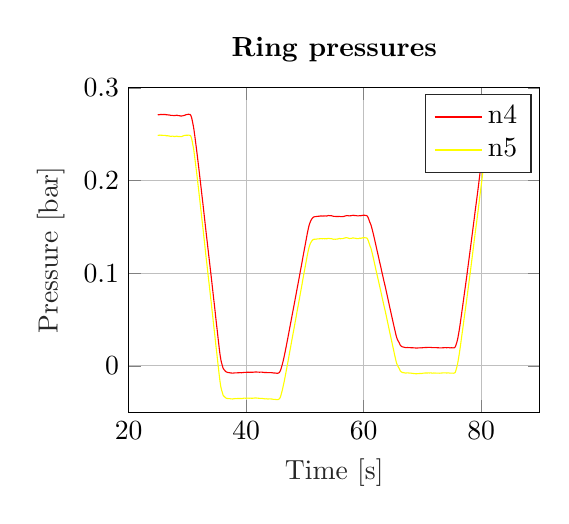
\begin{tikzpicture}

\begin{axis}[%
width=2.0556in,
height=1.62135in,
at={(1.011in,0.642in)},
scale only axis,
xmin=20,
xmax=90,
xlabel style={font=\color{white!15!black}},
xlabel={Time [s]},
ymin=-0.05,
ymax=0.3,
ylabel style={font=\color{white!15!black}},
ylabel={Pressure [bar]},
axis background/.style={fill=white},
title style={font=\bfseries},
title={Ring pressures},
xmajorgrids,
ymajorgrids,
legend style={legend cell align=left, align=left, draw=white!15!black}
]
\addplot [color=red]
  table[row sep=crcr]{%
24.95	0.27129154447703\\
25	0.271059384164224\\
25.05	0.270979960899317\\
25.1	0.270949413489738\\
25.15	0.270894428152494\\
25.2	0.271004398826981\\
25.25	0.271151026392963\\
25.3	0.271175464320627\\
25.35	0.271218230694038\\
25.4	0.271248778103618\\
25.45	0.271224340175954\\
25.5	0.271193792766375\\
25.55	0.271224340175954\\
25.6	0.271309872922777\\
25.65	0.271297653958946\\
25.7	0.271236559139786\\
25.75	0.271218230694038\\
25.8	0.271181573802543\\
25.85	0.271157135874879\\
25.9	0.27123044965787\\
25.95	0.27129154447703\\
26	0.271242668621702\\
26.05	0.271212121212123\\
26.1	0.271236559139786\\
26.15	0.271242668621702\\
26.2	0.271248778103618\\
26.25	0.271212121212123\\
26.3	0.271108260019552\\
26.35	0.270992179863149\\
26.4	0.270918866080158\\
26.45	0.271004398826981\\
26.5	0.271034946236561\\
26.55	0.27093108504399\\
26.6	0.270918866080158\\
26.65	0.270882209188663\\
26.7	0.270839442815251\\
26.75	0.270784457478008\\
26.8	0.270753910068428\\
26.85	0.270760019550344\\
26.9	0.270717253176933\\
26.95	0.270668377321605\\
27	0.270588954056698\\
27.05	0.270509530791791\\
27.1	0.2704362170088\\
27.15	0.270326246334313\\
27.2	0.270265151515154\\
27.25	0.270314027370481\\
27.3	0.270344574780061\\
27.35	0.270350684261977\\
27.4	0.270350684261977\\
27.45	0.270381231671557\\
27.5	0.270381231671557\\
27.55	0.270252932551322\\
27.6	0.270124633431087\\
27.65	0.270032991202348\\
27.7	0.269990224828936\\
27.75	0.270075757575759\\
27.8	0.270161290322583\\
27.85	0.270191837732162\\
27.9	0.270216275659826\\
27.95	0.270185728250246\\
28	0.270246823069406\\
28.05	0.270356793743893\\
28.1	0.270393450635389\\
28.15	0.270430107526884\\
28.2	0.270454545454548\\
28.25	0.270442326490715\\
28.3	0.270320136852397\\
28.35	0.270167399804498\\
28.4	0.27011852394917\\
28.45	0.270069648093842\\
28.5	0.269990224828935\\
28.55	0.269996334310851\\
28.6	0.269990224828934\\
28.65	0.269916911045943\\
28.7	0.269843597262951\\
28.75	0.269855816226783\\
28.8	0.269794721407624\\
28.85	0.269641984359725\\
28.9	0.269654203323557\\
28.95	0.269672531769304\\
29	0.269629765395892\\
29.05	0.269684750733136\\
29.1	0.269788611925707\\
29.15	0.269831378299118\\
29.2	0.269861925708698\\
29.25	0.269965786901269\\
29.3	0.270014662756597\\
29.35	0.27003910068426\\
29.4	0.270167399804495\\
29.45	0.270314027370478\\
29.5	0.270393450635385\\
29.55	0.270466764418376\\
29.6	0.270601173020526\\
29.65	0.270705034213097\\
29.7	0.270821114369499\\
29.75	0.271047165200389\\
29.8	0.271175464320624\\
29.85	0.271163245356792\\
29.9	0.271163245356793\\
29.95	0.271230449657868\\
30	0.271352639296187\\
30.05	0.27140762463343\\
30.1	0.271444281524926\\
30.15	0.271542033235581\\
30.2	0.271505376344086\\
30.25	0.271444281524926\\
30.3	0.27143817204301\\
30.35	0.271334310850439\\
30.4	0.271260997067448\\
30.45	0.271230449657868\\
30.5	0.271041055718474\\
30.55	0.270588954056695\\
30.6	0.26987414467253\\
30.65	0.269012707722383\\
30.7	0.268047409579666\\
30.75	0.266837732160311\\
30.8	0.26539589442815\\
30.85	0.26378910068426\\
30.9	0.262176197458453\\
30.95	0.260593841642226\\
31	0.258987047898335\\
31.05	0.257233626588462\\
31.1	0.255229716520036\\
31.15	0.252975317693056\\
31.2	0.250629276637338\\
31.25	0.248283235581619\\
31.3	0.245869990224825\\
31.35	0.24341397849462\\
31.4	0.240945747800582\\
31.45	0.238477517106545\\
31.5	0.236015395894423\\
31.55	0.233547165200386\\
31.6	0.231036168132937\\
31.65	0.228482404692077\\
31.7	0.225824780058645\\
31.75	0.223136608015635\\
31.8	0.220478983382204\\
31.85	0.217827468230688\\
31.9	0.215175953079173\\
31.95	0.212481671554246\\
32	0.209769061583572\\
32.05	0.207062561094813\\
32.1	0.204349951124139\\
32.15	0.201649560117296\\
32.2	0.198906402737042\\
32.25	0.196132697947208\\
32.3	0.19339565004887\\
32.35	0.190658602150532\\
32.4	0.187921554252194\\
32.45	0.18514784946236\\
32.5	0.18236803519061\\
32.55	0.17964931573802\\
32.6	0.176912267839682\\
32.65	0.174163000977513\\
32.7	0.171346529814267\\
32.75	0.168462854349946\\
32.8	0.165609726295205\\
32.85	0.16279325513196\\
32.9	0.159989002932547\\
32.95	0.157178641251217\\
33	0.15431940371456\\
33.05	0.151380742912996\\
33.1	0.148435972629516\\
33.15	0.145582844574775\\
33.2	0.14282746823069\\
33.25	0.140096529814268\\
33.3	0.137377810361678\\
33.35	0.134652981427172\\
33.4	0.131903714565002\\
33.45	0.129123900293252\\
33.5	0.126337976539587\\
33.55	0.123558162267838\\
33.6	0.12085166177908\\
33.65	0.118126832844574\\
33.7	0.115377565982404\\
33.75	0.112622189638318\\
33.8	0.1098545943304\\
33.85	0.107111436950146\\
33.9	0.104337732160313\\
33.95	0.101594574780059\\
34	0.0988575268817211\\
34.05	0.0960899315738033\\
34.1	0.0932490224828939\\
34.15	0.0904325513196486\\
34.2	0.0876527370478989\\
34.25	0.0848057184750736\\
34.3	0.0819831378299124\\
34.35	0.0791727761485831\\
34.4	0.0763196480938419\\
34.45	0.0734481915933529\\
34.5	0.0706439393939395\\
34.55	0.0678885630498538\\
34.6	0.0650782013685244\\
34.65	0.0622617302052792\\
34.7	0.0594024926686224\\
34.75	0.0564332844574786\\
34.8	0.0534762952101666\\
34.85	0.0506048387096776\\
34.9	0.0477578201368523\\
34.95	0.0449596774193548\\
35	0.0421493157380255\\
35.05	0.0393328445747802\\
35.1	0.0365224828934508\\
35.15	0.0336449169110459\\
35.2	0.0308223362658847\\
35.25	0.0280303030303031\\
35.3	0.0252565982404693\\
35.35	0.0225378787878793\\
35.4	0.0197947214076255\\
35.45	0.0170760019550354\\
35.5	0.014552785923755\\
35.55	0.0122311827957002\\
35.6	0.0101050830889555\\
35.65	0.00814393939394122\\
35.7	0.00634164222874105\\
35.75	0.00480816226784171\\
35.8	0.00350684261974799\\
35.85	0.00234604105572096\\
35.9	0.00117913000977801\\
35.95	4.27663734146933e-05\\
36	-0.00106304985336898\\
36.05	-0.00208944281524559\\
36.1	-0.00289589442814879\\
36.15	-0.00342130987291895\\
36.2	-0.00384897360703427\\
36.25	-0.00430718475072922\\
36.3	-0.0046737536656849\\
36.35	-0.00499755620722908\\
36.4	-0.00535801564026883\\
36.45	-0.00571236559139265\\
36.5	-0.0060056207233572\\
36.55	-0.0062683284457421\\
36.6	-0.00648826979471551\\
36.65	-0.00666544477027742\\
36.7	-0.00682429130009155\\
36.75	-0.00694037145649418\\
36.8	-0.00703812316714902\\
36.85	-0.00713587487780387\\
36.9	-0.00722140762462686\\
36.95	-0.00728250244378614\\
37	-0.00731915933528171\\
37.05	-0.00738025415444099\\
37.1	-0.0074046920821047\\
37.15	-0.00742302052785249\\
37.2	-0.00748411534701177\\
37.25	-0.00753910068425512\\
37.3	-0.00760630498533033\\
37.35	-0.00767350928640553\\
37.4	-0.00772238514173296\\
37.45	-0.00774071358748074\\
37.5	-0.00775904203322852\\
37.55	-0.00781402737047188\\
37.6	-0.00785679374388337\\
37.65	-0.00788123167154708\\
37.7	-0.00787512218963116\\
37.75	-0.00783846529813559\\
37.8	-0.0078201368523878\\
37.85	-0.00779569892472409\\
37.9	-0.00776515151514445\\
37.95	-0.00772238514173296\\
38	-0.00766129032257368\\
38.05	-0.00759408602149847\\
38.1	-0.0075574291300029\\
38.15	-0.00756353861191883\\
38.2	-0.00757575757575069\\
38.25	-0.00759408602149847\\
38.3	-0.00761241446724625\\
38.35	-0.00762463343107811\\
38.4	-0.00762463343107811\\
38.45	-0.00759408602149847\\
38.5	-0.00754521016617105\\
38.55	-0.00753299120233919\\
38.6	-0.00753299120233919\\
38.65	-0.00747800586509584\\
38.7	-0.0074474584555162\\
38.75	-0.00746578690126398\\
38.8	-0.00745356793743213\\
38.85	-0.00742913000976841\\
38.9	-0.0074046920821047\\
38.95	-0.00738636363635692\\
39	-0.00737414467252506\\
39.05	-0.00739247311827285\\
39.1	-0.00743523949168434\\
39.15	-0.0074474584555162\\
39.2	-0.0074474584555162\\
39.25	-0.00742913000976841\\
39.3	-0.00739858260018877\\
39.35	-0.00736803519060913\\
39.4	-0.00734359726294542\\
39.45	-0.00730083088953393\\
39.5	-0.00722140762462686\\
39.55	-0.00717864125121537\\
39.6	-0.00714809384163573\\
39.65	-0.0070992179863083\\
39.7	-0.00708088954056052\\
39.75	-0.00708699902247645\\
39.8	-0.00708699902247645\\
39.85	-0.00708699902247645\\
39.9	-0.00711143695014016\\
39.95	-0.00710532746822423\\
40	-0.00705645161289681\\
40.05	-0.00700146627565346\\
40.1	-0.00695869990224196\\
40.15	-0.0069464809384101\\
40.2	-0.00695869990224196\\
40.25	-0.00699535679373753\\
40.3	-0.0069892473118216\\
40.35	-0.00697091886607382\\
40.4	-0.0069892473118216\\
40.45	-0.00699535679373753\\
40.5	-0.00700146627565346\\
40.55	-0.00701368523948531\\
40.6	-0.00700146627565346\\
40.65	-0.00695259042032603\\
40.7	-0.0069464809384101\\
40.75	-0.00697702834798974\\
40.8	-0.00697091886607382\\
40.85	-0.00697091886607382\\
40.9	-0.0069892473118216\\
40.95	-0.00699535679373753\\
41	-0.00698313782990567\\
41.05	-0.00696480938415789\\
41.1	-0.0069464809384101\\
41.15	-0.00694037145649418\\
41.2	-0.00691593352883046\\
41.25	-0.00686705767350304\\
41.3	-0.00686705767350304\\
41.35	-0.00686705767350304\\
41.4	-0.00681207233625969\\
41.45	-0.00673264907135263\\
41.5	-0.00667766373410927\\
41.55	-0.00665322580644556\\
41.6	-0.00665322580644556\\
41.65	-0.00667155425219335\\
41.7	-0.00669599217985706\\
41.75	-0.0067265395894367\\
41.8	-0.00672043010752077\\
41.85	-0.00672043010752077\\
41.9	-0.00675708699901634\\
41.95	-0.00678152492668005\\
42	-0.00679985337242783\\
42.05	-0.00680596285434376\\
42.1	-0.00681818181817562\\
42.15	-0.00685483870967118\\
42.2	-0.0068792766373349\\
42.25	-0.00689149560116675\\
42.3	-0.00689760508308268\\
42.35	-0.00688538611925082\\
42.4	-0.00686705767350304\\
42.45	-0.00685483870967118\\
42.5	-0.00684261974583933\\
42.55	-0.0068365102639234\\
42.6	-0.00684261974583933\\
42.65	-0.00686094819158711\\
42.7	-0.0068792766373349\\
42.75	-0.00691593352883046\\
42.8	-0.00695259042032603\\
42.85	-0.0069892473118216\\
42.9	-0.00701368523948531\\
42.95	-0.00705034213098088\\
43	-0.00711143695014016\\
43.05	-0.00716642228738351\\
43.1	-0.00720918866079501\\
43.15	-0.00723362658845872\\
43.2	-0.0072519550342065\\
43.25	-0.0072519550342065\\
43.3	-0.00722751710654279\\
43.35	-0.00720918866079501\\
43.4	-0.00719696969696315\\
43.45	-0.00720307917887908\\
43.5	-0.0072519550342065\\
43.55	-0.00727639296187022\\
43.6	-0.00728861192570207\\
43.65	-0.00732526881719764\\
43.7	-0.00734359726294542\\
43.75	-0.00732526881719764\\
43.8	-0.00731915933528171\\
43.85	-0.00731304985336578\\
43.9	-0.00731304985336578\\
43.95	-0.00732526881719764\\
44	-0.00734970674486135\\
44.05	-0.00735581622677728\\
44.1	-0.00733137829911357\\
44.15	-0.00733748778102949\\
44.2	-0.00736803519060913\\
44.25	-0.00738636363635692\\
44.3	-0.00739247311827285\\
44.35	-0.00742302052785249\\
44.4	-0.00743523949168434\\
44.45	-0.00745967741934805\\
44.5	-0.0075574291300029\\
44.55	-0.00761852394916218\\
44.6	-0.00764296187682589\\
44.65	-0.00769183773215332\\
44.7	-0.00771627565981703\\
44.75	-0.00771627565981703\\
44.8	-0.00771627565981703\\
44.85	-0.00774071358748074\\
44.9	-0.00775904203322852\\
44.95	-0.00780180840664002\\
45	-0.0078629032257993\\
45.05	-0.0079056695992108\\
45.1	-0.00793621700879044\\
45.15	-0.00796065493645415\\
45.2	-0.007972873900286\\
45.25	-0.00796676441837008\\
45.3	-0.00799120234603379\\
45.35	-0.00799731182794972\\
45.4	-0.00796676441837008\\
45.45	-0.00792399804495858\\
45.5	-0.00778958944280816\\
45.55	-0.00760630498533033\\
45.6	-0.00738025415444099\\
45.65	-0.00713587487780387\\
45.7	-0.00672653958943634\\
45.75	-0.00612781036167469\\
45.8	-0.00548020527858561\\
45.85	-0.00474095796675762\\
45.9	-0.00382453567936771\\
45.95	-0.00282258064515482\\
46	-0.00183284457477377\\
46.05	-0.000763685239485667\\
46.1	0.00036045943304579\\
46.15	0.00150293255132503\\
46.2	0.00271260997067984\\
46.25	0.00400782013685799\\
46.3	0.00533357771261578\\
46.35	0.00665933528837357\\
46.4	0.00804618768329064\\
46.45	0.00947580645161921\\
46.5	0.0109359726295274\\
46.55	0.0125122189638383\\
46.6	0.0140762463343172\\
46.65	0.0156280547409644\\
46.7	0.0172104105571911\\
46.75	0.0188172043010816\\
46.8	0.0204178885630562\\
46.85	0.0220369012707785\\
46.9	0.0236925708699964\\
46.95	0.0253176930596347\\
47	0.0269550342131048\\
47.05	0.028586265884659\\
47.1	0.0302113880742972\\
47.15	0.031879276637347\\
47.2	0.0335960410557242\\
47.25	0.0353005865102695\\
47.3	0.0369745845552352\\
47.35	0.0386791300097805\\
47.4	0.040371456500494\\
47.45	0.0420393450635437\\
47.5	0.0437561094819209\\
47.55	0.0454239980449707\\
47.6	0.0470735581622726\\
47.65	0.0487658846529861\\
47.7	0.0504093352883722\\
47.75	0.0520833333333378\\
47.8	0.0537939882697991\\
47.85	0.0554679863147648\\
47.9	0.057099217986319\\
47.95	0.0587854349951165\\
48	0.0605021994134937\\
48.05	0.0621334310850479\\
48.1	0.063770772238518\\
48.15	0.0654569892473155\\
48.2	0.0671126588465334\\
48.25	0.068798875855331\\
48.3	0.0705522971652037\\
48.35	0.0722751710654968\\
48.4	0.0739491691104625\\
48.45	0.0756292766373441\\
48.5	0.0773093841642258\\
48.55	0.0790383675464348\\
48.6	0.0807917888563075\\
48.65	0.0825146627566006\\
48.7	0.0842130987292301\\
48.75	0.0858809872922798\\
48.8	0.0875610948191614\\
48.85	0.0892106549364634\\
48.9	0.090890762463345\\
48.95	0.0926014173998063\\
49	0.0942998533724357\\
49.05	0.0960166177908128\\
49.1	0.0977517106549378\\
49.15	0.0994990224828946\\
49.2	0.101246334310851\\
49.25	0.10300586510264\\
49.3	0.104679863147606\\
49.35	0.106335532746824\\
49.4	0.108015640273705\\
49.45	0.109738514173998\\
49.5	0.111516373411535\\
49.55	0.113269794721408\\
49.6	0.115047653958944\\
49.65	0.116837732160312\\
49.7	0.118585043988269\\
49.75	0.120307917888562\\
49.8	0.122030791788855\\
49.85	0.123747556207233\\
49.9	0.125470430107526\\
49.95	0.127168866080155\\
50	0.128848973607037\\
50.05	0.130510752688171\\
50.1	0.132160312805473\\
50.15	0.133870967741934\\
50.2	0.135667155425218\\
50.25	0.137414467253175\\
50.3	0.139106793743888\\
50.35	0.140823558162266\\
50.4	0.142485337243399\\
50.45	0.14409213098729\\
50.5	0.145650048875853\\
50.55	0.147146871945257\\
50.6	0.148545943304006\\
50.65	0.149957233626586\\
50.7	0.15125855327468\\
50.75	0.15230938416422\\
50.8	0.153262463343106\\
50.85	0.154191104594328\\
50.9	0.155009775171063\\
50.95	0.155742913000975\\
51	0.156476050830887\\
51.05	0.157129765395892\\
51.1	0.157728494623654\\
51.15	0.158284457478004\\
51.2	0.158760997067446\\
51.25	0.159121456500486\\
51.3	0.159500244379274\\
51.35	0.159921798631473\\
51.4	0.160221163245353\\
51.45	0.160477761485822\\
51.5	0.160654936461384\\
51.55	0.160709921798627\\
51.6	0.160807673509282\\
51.65	0.160929863147601\\
51.7	0.161003176930592\\
51.75	0.161015395894424\\
51.8	0.160997067448676\\
51.85	0.160997067448676\\
51.9	0.161045943304003\\
51.95	0.16115591397849\\
52	0.161223118279565\\
52.05	0.161259775171061\\
52.1	0.161314760508304\\
52.15	0.1613514173998\\
52.2	0.161375855327464\\
52.25	0.161424731182791\\
52.3	0.16148582600195\\
52.35	0.161467497556202\\
52.4	0.161449169110455\\
52.45	0.161510263929614\\
52.5	0.16154692082111\\
52.55	0.161614125122185\\
52.6	0.161705767350924\\
52.65	0.161754643206251\\
52.7	0.161779081133915\\
52.75	0.161736314760503\\
52.8	0.161705767350924\\
52.85	0.161693548387092\\
52.9	0.161656891495596\\
52.95	0.161626344086017\\
53	0.161620234604101\\
53.05	0.16165078201368\\
53.1	0.161730205278587\\
53.15	0.161754643206251\\
53.2	0.161736314760503\\
53.25	0.161742424242419\\
53.3	0.161730205278587\\
53.35	0.161766862170083\\
53.4	0.161785190615831\\
53.45	0.161791300097747\\
53.5	0.161821847507326\\
53.55	0.161742424242419\\
53.6	0.161705767350924\\
53.65	0.161699657869008\\
53.7	0.161693548387092\\
53.75	0.161754643206251\\
53.8	0.161827956989242\\
53.85	0.161944037145645\\
53.9	0.162047898338216\\
53.95	0.162090664711627\\
54	0.162170087976534\\
54.05	0.162218963831862\\
54.1	0.162170087976534\\
54.15	0.162157869012702\\
54.2	0.162133431085039\\
54.25	0.162005131964804\\
54.3	0.161986803519056\\
54.35	0.162047898338216\\
54.4	0.162072336265879\\
54.45	0.162115102639291\\
54.5	0.162133431085039\\
54.55	0.162047898338216\\
54.6	0.161858504398822\\
54.65	0.161699657869008\\
54.7	0.161656891495596\\
54.75	0.161608015640269\\
54.8	0.161498044965782\\
54.85	0.161412512218959\\
54.9	0.161339198435968\\
54.95	0.161278103616809\\
55	0.161265884652977\\
55.05	0.161290322580641\\
55.1	0.161265884652977\\
55.15	0.161247556207229\\
55.2	0.161204789833818\\
55.25	0.16118646138807\\
55.3	0.161210899315734\\
55.35	0.161162023460406\\
55.4	0.16115591397849\\
55.45	0.161217008797649\\
55.5	0.161198680351902\\
55.55	0.161125366568911\\
55.6	0.161162023460406\\
55.65	0.161192570869986\\
55.7	0.161149804496574\\
55.75	0.161217008797649\\
55.8	0.161326979472136\\
55.85	0.161326979472136\\
55.9	0.161247556207229\\
55.95	0.161174242424238\\
56	0.161119257086995\\
56.05	0.161052052785919\\
56.1	0.161009286412508\\
56.15	0.161033724340172\\
56.2	0.161039833822088\\
56.25	0.161052052785919\\
56.3	0.161070381231667\\
56.35	0.161070381231667\\
56.4	0.161119257086995\\
56.45	0.161094819159331\\
56.5	0.161094819159331\\
56.55	0.161180351906154\\
56.6	0.161271994134893\\
56.65	0.161345307917884\\
56.7	0.161406402737043\\
56.75	0.161522482893446\\
56.8	0.161620234604101\\
56.85	0.161693548387092\\
56.9	0.161791300097747\\
56.95	0.161870723362654\\
57	0.161962365591393\\
57.05	0.162054007820132\\
57.1	0.162115102639291\\
57.15	0.162170087976534\\
57.2	0.16214565004887\\
57.25	0.162078445747795\\
57.3	0.162035679374384\\
57.35	0.16201124144672\\
57.4	0.161986803519056\\
57.45	0.161925708699897\\
57.5	0.161858504398822\\
57.55	0.161821847507326\\
57.6	0.161821847507326\\
57.65	0.16187683284457\\
57.7	0.161968475073309\\
57.75	0.162035679374384\\
57.8	0.162023460410552\\
57.85	0.162005131964804\\
57.9	0.162054007820132\\
57.95	0.162115102639291\\
58	0.16220674486803\\
58.05	0.162353372434012\\
58.1	0.162432795698919\\
58.15	0.162451124144667\\
58.2	0.162481671554247\\
58.25	0.162475562072331\\
58.3	0.162390029325508\\
58.35	0.162255620723357\\
58.4	0.162231182795693\\
58.45	0.162249511241441\\
58.5	0.162218963831862\\
58.55	0.162231182795693\\
58.6	0.162151759530786\\
58.65	0.162066226783963\\
58.7	0.162072336265879\\
58.75	0.162054007820132\\
58.8	0.162029569892468\\
58.85	0.16198069403714\\
58.9	0.161889051808402\\
58.95	0.161889051808402\\
59	0.161882942326486\\
59.05	0.161864613880738\\
59.1	0.161907380254149\\
59.15	0.161864613880738\\
59.2	0.16187683284457\\
59.25	0.161992913000972\\
59.3	0.162047898338216\\
59.35	0.162084555229711\\
59.4	0.162102883675459\\
59.45	0.162023460410552\\
59.5	0.161944037145645\\
59.55	0.161986803519056\\
59.6	0.162102883675459\\
59.65	0.162225073313778\\
59.7	0.162255620723357\\
59.75	0.162273949169105\\
59.8	0.162353372434012\\
59.85	0.162420576735087\\
59.9	0.162463343108499\\
59.95	0.162499999999994\\
60	0.162518328445742\\
60.05	0.162518328445742\\
60.1	0.162561094819154\\
60.15	0.162561094819154\\
60.2	0.162487781036162\\
60.25	0.162383919843592\\
60.3	0.162328934506348\\
60.35	0.162292277614853\\
60.4	0.162231182795693\\
60.45	0.162200635386114\\
60.5	0.162127321603123\\
60.55	0.161992913000972\\
60.6	0.161699657869008\\
60.65	0.161284213098725\\
60.7	0.160777126099702\\
60.75	0.16010508308895\\
60.8	0.159359726295206\\
60.85	0.158596041055714\\
60.9	0.157771260997063\\
60.95	0.156867057673505\\
61	0.155913978494619\\
61.05	0.155003665689145\\
61.1	0.154294965786897\\
61.15	0.153653470185724\\
61.2	0.152871456500484\\
61.25	0.152028347996086\\
61.3	0.151020283479957\\
61.35	0.149780058651023\\
61.4	0.148570381231668\\
61.45	0.147415689149557\\
61.5	0.146212121212118\\
61.55	0.144965786901268\\
61.6	0.143676686217006\\
61.65	0.142320381231669\\
61.7	0.140976295210163\\
61.75	0.139632209188657\\
61.8	0.138269794721404\\
61.85	0.136882942326487\\
61.9	0.135453323558158\\
61.95	0.134011485825998\\
62	0.132563538611922\\
62.05	0.131140029325509\\
62.1	0.129734848484844\\
62.15	0.128305229716516\\
62.2	0.126906158357767\\
62.25	0.12551930596285\\
62.3	0.124089687194521\\
62.35	0.122684506353856\\
62.4	0.121297653958939\\
62.45	0.119916911045938\\
62.5	0.118523949169105\\
62.55	0.11711876832844\\
62.6	0.115713587487775\\
62.65	0.114247311827951\\
62.7	0.112793255131959\\
62.75	0.111400293255126\\
62.8	0.110037878787873\\
62.85	0.108706011730199\\
62.9	0.107349706744861\\
62.95	0.105938416422281\\
63	0.104459921798625\\
63.05	0.102956989247305\\
63.1	0.101490713587481\\
63.15	0.100091642228732\\
63.2	0.0987292277614785\\
63.25	0.0973240469208136\\
63.3	0.0959188660801488\\
63.35	0.0945320136852317\\
63.4	0.093108504398819\\
63.45	0.0916972140762383\\
63.5	0.0903409090909008\\
63.55	0.0890090420332271\\
63.6	0.0876893939393852\\
63.65	0.0863391984359637\\
63.7	0.084921798631467\\
63.75	0.0834860703812225\\
63.8	0.0820442326490621\\
63.85	0.0806085043988176\\
63.9	0.0792094330400687\\
63.95	0.0777492668621605\\
64	0.0762707722385045\\
64.05	0.0748106060605963\\
64.1	0.0733443304007722\\
64.15	0.0719330400781914\\
64.2	0.0704728739002832\\
64.25	0.0689821603127953\\
64.3	0.067528103616803\\
64.35	0.0660434995112311\\
64.4	0.0645588954056592\\
64.45	0.0631414956011625\\
64.5	0.0617302052785817\\
64.55	0.0603005865102531\\
64.6	0.0588831867057564\\
64.65	0.057441348973596\\
64.7	0.0560178396871834\\
64.75	0.0546004398826867\\
64.8	0.0531586021505262\\
64.85	0.0517167644183658\\
64.9	0.0502932551319532\\
64.95	0.0489064027370361\\
65	0.0475012218963713\\
65.05	0.0460654936461268\\
65.1	0.04464809384163\\
65.15	0.0432184750733015\\
65.2	0.0418010752688048\\
65.25	0.0404264418377196\\
65.3	0.0390334799608866\\
65.35	0.0376710654936332\\
65.4	0.0363086510263798\\
65.45	0.0348790322580513\\
65.5	0.0335288367546298\\
65.55	0.0323252688171905\\
65.6	0.0312255620723221\\
65.65	0.0301869501466129\\
65.7	0.0292827468230545\\
65.75	0.0285068426197309\\
65.8	0.0277798142717348\\
65.85	0.0271138807428979\\
65.9	0.0265456989247159\\
65.95	0.0260386119256932\\
66	0.0255620723362501\\
66.05	0.0250733137829752\\
66.1	0.0243707233626427\\
66.15	0.0235459433039917\\
66.2	0.022873900293239\\
66.25	0.0222751710654773\\
66.3	0.021816959921782\\
66.35	0.0215786901270601\\
66.4	0.0212976539589267\\
66.45	0.0210227272727092\\
66.5	0.0208516617790629\\
66.55	0.0206622678396688\\
66.6	0.0204850928641065\\
66.65	0.0204178885630313\\
66.7	0.0203690127077039\\
66.75	0.0202529325513012\\
66.8	0.0201612903225623\\
66.85	0.0201124144672349\\
66.9	0.0200085532746641\\
66.95	0.0199230205278411\\
67	0.0198741446725137\\
67.05	0.0198130498533544\\
67.1	0.0197275171065314\\
67.15	0.0196603128054562\\
67.2	0.0196542033235403\\
67.25	0.0196603128054562\\
67.3	0.019678641251204\\
67.35	0.0197091886607836\\
67.4	0.0197214076246155\\
67.45	0.0197152981426996\\
67.5	0.0197275171065314\\
67.55	0.0197275171065314\\
67.6	0.0196847507331199\\
67.65	0.0196297653958766\\
67.7	0.0195869990224651\\
67.75	0.0195808895405492\\
67.8	0.0196053274682129\\
67.85	0.0196236559139606\\
67.9	0.0196175464320447\\
67.95	0.019593108504381\\
68	0.0195625610948014\\
68.05	0.0195442326490536\\
68.1	0.0195442326490536\\
68.15	0.0195381231671377\\
68.2	0.0195136852394739\\
68.25	0.0195014662756421\\
68.3	0.0195197947213899\\
68.35	0.0195381231671377\\
68.4	0.0195197947213899\\
68.45	0.0194770283479784\\
68.5	0.019422043010735\\
68.55	0.0193731671554076\\
68.6	0.019336510263912\\
68.65	0.0193181818181642\\
68.7	0.0193059628543324\\
68.75	0.0192937438905005\\
68.8	0.0192448680351731\\
68.85	0.0192082111436775\\
68.9	0.0191776637340979\\
68.95	0.0191532258064342\\
69	0.019171554252182\\
69.05	0.0192021016617616\\
69.1	0.0192448680351731\\
69.15	0.019250977517089\\
69.2	0.019257086999005\\
69.25	0.0192876344085846\\
69.3	0.0192937438905005\\
69.35	0.0192937438905005\\
69.4	0.019342619745828\\
69.45	0.019336510263912\\
69.5	0.0193548387096598\\
69.55	0.019422043010735\\
69.6	0.0194464809383987\\
69.65	0.0194464809383987\\
69.7	0.019428152492651\\
69.75	0.0194037145649872\\
69.8	0.0193853861192395\\
69.85	0.0194159335288191\\
69.9	0.0194586999022306\\
69.95	0.0194770283479784\\
70	0.0194953567937262\\
70.05	0.0195442326490536\\
70.1	0.0195747800586332\\
70.15	0.0196114369501288\\
70.2	0.0196480938416244\\
70.25	0.019678641251204\\
70.3	0.0196969696969518\\
70.35	0.0196969696969518\\
70.4	0.0197336265884474\\
70.45	0.0197702834799429\\
70.5	0.0198008308895226\\
70.55	0.0198252688171863\\
70.6	0.0198313782991022\\
70.65	0.0198252688171863\\
70.7	0.0198069403714385\\
70.75	0.0198069403714385\\
70.8	0.0198069403714385\\
70.85	0.0198252688171863\\
70.9	0.0198619257086818\\
70.95	0.0198802541544296\\
71	0.0199046920820933\\
71.05	0.0199169110459252\\
71.1	0.0198924731182615\\
71.15	0.0198619257086818\\
71.2	0.0198619257086818\\
71.25	0.0198863636363456\\
71.3	0.0199046920820933\\
71.35	0.0199046920820933\\
71.4	0.0198924731182615\\
71.45	0.0198558162267659\\
71.5	0.0198069403714385\\
71.55	0.0197825024437748\\
71.6	0.0197336265884474\\
71.65	0.0196725317692881\\
71.7	0.0196236559139606\\
71.75	0.0196236559139606\\
71.8	0.0196419843597084\\
71.85	0.0196480938416244\\
71.9	0.0196847507331199\\
71.95	0.0196603128054562\\
72	0.0196358748777925\\
72.05	0.0196358748777925\\
72.1	0.0196297653958766\\
72.15	0.0196419843597084\\
72.2	0.0196480938416244\\
72.25	0.0196419843597084\\
72.3	0.0196480938416244\\
72.35	0.0196419843597084\\
72.4	0.0196236559139606\\
72.45	0.0195992179862969\\
72.5	0.0195442326490536\\
72.55	0.0195259042033058\\
72.6	0.0195197947213899\\
72.65	0.0195381231671377\\
72.7	0.0195564516128854\\
72.75	0.0195136852394739\\
72.8	0.0194586999022306\\
72.85	0.0194159335288191\\
72.9	0.0193976050830713\\
72.95	0.0193976050830713\\
73	0.0193914956011554\\
73.05	0.0193914956011554\\
73.1	0.0193853861192395\\
73.15	0.0193792766373235\\
73.2	0.0193914956011554\\
73.25	0.0193914956011554\\
73.3	0.0193792766373235\\
73.35	0.0193976050830713\\
73.4	0.0194403714564828\\
73.45	0.0194770283479784\\
73.5	0.019507575757558\\
73.55	0.0195136852394739\\
73.6	0.0195259042033058\\
73.65	0.0195442326490536\\
73.7	0.0195686705767173\\
73.75	0.0195747800586332\\
73.8	0.0196053274682129\\
73.85	0.0196236559139606\\
73.9	0.0196358748777925\\
73.95	0.0196480938416244\\
74	0.0196053274682129\\
74.05	0.0195564516128854\\
74.1	0.0195259042033058\\
74.15	0.0195381231671377\\
74.2	0.0195564516128854\\
74.25	0.0195869990224651\\
74.3	0.0196297653958766\\
74.35	0.0196542033235403\\
74.4	0.0196480938416244\\
74.45	0.0196419843597084\\
74.5	0.0196297653958766\\
74.55	0.0195808895405492\\
74.6	0.019507575757558\\
74.65	0.0194464809383987\\
74.7	0.0194159335288191\\
74.75	0.0194159335288191\\
74.8	0.0194403714564828\\
74.85	0.0194770283479784\\
74.9	0.0194770283479784\\
74.95	0.0194586999022306\\
75	0.0194525904203147\\
75.05	0.0194342619745669\\
75.1	0.0194464809383987\\
75.15	0.0194403714564828\\
75.2	0.0194403714564828\\
75.25	0.019428152492651\\
75.3	0.019428152492651\\
75.35	0.0194648093841465\\
75.4	0.0194709188660624\\
75.45	0.0195320136852217\\
75.5	0.0197397360703636\\
75.55	0.0200635386119085\\
75.6	0.0205156402736879\\
75.65	0.0211571358748611\\
75.7	0.0220246823069239\\
75.75	0.0229960899315575\\
75.8	0.0239613880742752\\
75.85	0.0249938905180684\\
75.9	0.0261363636363484\\
75.95	0.027394916911031\\
76	0.0287756598240321\\
76.05	0.0303091397849315\\
76.1	0.0320014662756453\\
76.15	0.0337976539589302\\
76.2	0.0355938416422152\\
76.25	0.0374572336265754\\
76.3	0.0394061583577585\\
76.35	0.041410068426185\\
76.4	0.0435178396871823\\
76.45	0.0456989247311707\\
76.5	0.0479411045943184\\
76.55	0.0502260508308776\\
76.6	0.0525354349951005\\
76.65	0.0548203812316597\\
76.7	0.0571053274682189\\
76.75	0.0594330400781896\\
76.8	0.0617118768328329\\
76.85	0.0639662756598124\\
76.9	0.0662695503421194\\
76.95	0.0685850439882582\\
77	0.0708516617790696\\
77.05	0.0731549364613766\\
77.1	0.0755254154447588\\
77.15	0.0778592375366454\\
77.2	0.0801441837732046\\
77.25	0.0824291300097638\\
77.3	0.0847079667644071\\
77.35	0.0869684750733025\\
77.4	0.0892778592375255\\
77.45	0.0916239002932439\\
77.5	0.0939943792766261\\
77.55	0.0963465298142605\\
77.6	0.0987353372433905\\
77.65	0.101191348973596\\
77.7	0.103653470185717\\
77.75	0.106072825024426\\
77.8	0.108431085043977\\
77.85	0.110789345063527\\
77.9	0.113227028347984\\
77.95	0.115689149560106\\
78	0.118120723362647\\
78.05	0.120509530791777\\
78.1	0.122916666666655\\
78.15	0.125354349951112\\
78.2	0.127755376344074\\
78.25	0.130199169110447\\
78.3	0.13270405669598\\
78.35	0.135239491691093\\
78.4	0.137719941348962\\
78.45	0.140145405669588\\
78.5	0.142570869990213\\
78.55	0.145020772238503\\
78.6	0.147507331378288\\
78.65	0.150024437927652\\
78.7	0.152468230694025\\
78.75	0.154924242424231\\
78.8	0.157435239491679\\
78.85	0.159909579667632\\
78.9	0.162420576735081\\
78.95	0.164974340175941\\
79	0.167460899315726\\
79.05	0.16987414467252\\
79.1	0.172281280547398\\
79.15	0.174670087976527\\
79.2	0.177071114369489\\
79.25	0.179472140762451\\
79.3	0.181873167155413\\
79.35	0.184353616813282\\
79.4	0.186834066471151\\
79.45	0.189302297165188\\
79.5	0.191758308895393\\
79.55	0.194269305962842\\
79.6	0.196933040078189\\
79.65	0.199572336265873\\
79.7	0.202144428152481\\
79.75	0.204771505376333\\
79.8	0.2074046920821\\
79.85	0.209921798631465\\
79.9	0.212316715542511\\
79.95	0.214809384164212\\
80	0.217338709677409\\
80.05	0.219794721407614\\
80.1	0.222336265884643\\
80.15	0.224938905180831\\
80.2	0.227510997067439\\
80.25	0.230040322580636\\
80.3	0.232545210166169\\
80.35	0.235062316715533\\
80.4	0.237640518084058\\
80.45	0.240194281524919\\
80.5	0.242613636363629\\
80.55	0.24484970674486\\
80.6	0.246902492668613\\
80.65	0.248833088954048\\
80.7	0.250507086999014\\
80.75	0.251985581622669\\
80.8	0.253500733137821\\
80.85	0.254991446725308\\
80.9	0.256366080156393\\
80.95	0.257642961876823\\
81	0.258791544477019\\
81.05	0.259775171065484\\
81.1	0.26063660801563\\
81.15	0.261443059628533\\
81.2	0.262237292277605\\
81.25	0.26282991202345\\
81.3	0.263361436950136\\
81.35	0.263917399804486\\
81.4	0.264326735092853\\
81.45	0.264687194525893\\
81.5	0.265035434995101\\
81.55	0.265273704789823\\
81.6	0.265450879765385\\
81.65	0.26574413489735\\
81.7	0.266049608993146\\
81.75	0.266275659824036\\
81.8	0.266556695992169\\
81.85	0.266782746823059\\
81.9	0.266941593352873\\
81.95	0.267173753665679\\
82	0.267393695014652\\
82.05	0.267625855327458\\
82.1	0.267931329423255\\
82.15	0.268169599217976\\
82.2	0.268334555229706\\
82.25	0.268572825024428\\
82.3	0.26878054740957\\
82.35	0.268988269794711\\
82.4	0.269183773216021\\
82.45	0.26930596285434\\
82.5	0.269379276637331\\
82.55	0.26947091886607\\
82.6	0.269586999022472\\
82.65	0.2696358748778\\
82.7	0.269599217986304\\
82.75	0.269623655913968\\
82.8	0.269788611925698\\
82.85	0.269898582600185\\
82.9	0.269929130009765\\
82.95	0.269947458455513\\
83	0.269941348973597\\
83.05	0.270032991202336\\
83.1	0.270136852394907\\
83.15	0.270167399804487\\
83.2	0.270259042033226\\
83.25	0.270283479960889\\
83.3	0.270246823069393\\
83.35	0.270210166177897\\
83.4	0.270185728250233\\
83.45	0.270216275659813\\
83.5	0.27035679374388\\
83.55	0.270466764418367\\
83.6	0.270527859237526\\
83.65	0.270564516129022\\
83.7	0.270564516129022\\
83.75	0.270637829912014\\
83.8	0.27064393939393\\
83.85	0.270656158357762\\
83.9	0.27070503421309\\
83.95	0.270711143695006\\
84	0.270827223851409\\
84.05	0.270992179863139\\
84.1	0.271041055718467\\
84.15	0.27109604105571\\
84.2	0.271236559139777\\
84.25	0.271340420332348\\
84.3	0.271407624633423\\
84.35	0.271425953079171\\
84.4	0.271395405669591\\
84.45	0.271346529814264\\
84.5	0.271340420332348\\
84.55	0.271315982404684\\
84.6	0.271206011730197\\
84.65	0.271077712609962\\
84.7	0.270906647116316\\
84.75	0.270723362658837\\
84.8	0.270570625610938\\
84.85	0.270478983382199\\
84.9	0.27055229716519\\
};
\addlegendentry{n4}

\addplot [color=mycolor1]
  table[row sep=crcr]{%
24.95	0.248979716520036\\
25	0.248851417399801\\
25.05	0.248753665689146\\
25.1	0.248668132942323\\
25.15	0.248710899315735\\
25.2	0.24883919843597\\
25.25	0.248979716520037\\
25.3	0.249077468230692\\
25.35	0.249053030303028\\
25.4	0.248961388074289\\
25.45	0.248912512218961\\
25.5	0.24886974584555\\
25.55	0.248851417399802\\
25.6	0.24883919843597\\
25.65	0.248863636363634\\
25.7	0.248875855327466\\
25.75	0.248784213098726\\
25.8	0.248698680351903\\
25.85	0.248704789833819\\
25.9	0.248717008797651\\
25.95	0.248729227761483\\
26	0.248753665689146\\
26.05	0.248741446725315\\
26.1	0.248735337243399\\
26.15	0.248747556207231\\
26.2	0.248765884652978\\
26.25	0.248717008797651\\
26.3	0.248576490713584\\
26.35	0.248399315738022\\
26.4	0.248271016617787\\
26.45	0.248264907135871\\
26.5	0.248301564027367\\
26.55	0.248313782991199\\
26.6	0.24832600195503\\
26.65	0.248307673509282\\
26.7	0.248246578690123\\
26.75	0.248167155425215\\
26.8	0.24813049853372\\
26.85	0.24806940371456\\
26.9	0.248014418377317\\
26.95	0.247996089931569\\
27	0.247916666666662\\
27.05	0.247800586510259\\
27.1	0.247708944281519\\
27.15	0.247635630498528\\
27.2	0.247629521016612\\
27.25	0.247715053763435\\
27.3	0.247782258064511\\
27.35	0.247849462365586\\
27.4	0.247898338220913\\
27.45	0.247880009775166\\
27.5	0.247849462365586\\
27.55	0.247825024437922\\
27.6	0.247727272727267\\
27.65	0.247611192570864\\
27.7	0.247513440860209\\
27.75	0.247489002932545\\
27.8	0.24755620723362\\
27.85	0.247537878787873\\
27.9	0.247519550342125\\
27.95	0.247580645161285\\
28	0.247629521016612\\
28.05	0.247751710654931\\
28.1	0.247880009775166\\
28.15	0.247898338220914\\
28.2	0.247849462365586\\
28.25	0.247763929618763\\
28.3	0.247684506353856\\
28.35	0.247598973607033\\
28.4	0.247489002932546\\
28.45	0.247421798631471\\
28.5	0.247434017595302\\
28.55	0.247489002932546\\
28.6	0.24751344086021\\
28.65	0.247464565004882\\
28.7	0.247427908113387\\
28.75	0.247446236559134\\
28.8	0.247440127077218\\
28.85	0.247360703812311\\
28.9	0.247311827956984\\
28.95	0.247354594330395\\
29	0.24742179863147\\
29.05	0.247531769305957\\
29.1	0.247702834799603\\
29.15	0.247892228738998\\
29.2	0.247996089931569\\
29.25	0.248130498533719\\
29.3	0.248271016617786\\
29.35	0.248313782991197\\
29.4	0.248417644183768\\
29.45	0.248558162267835\\
29.5	0.248698680351901\\
29.55	0.24875977517106\\
29.6	0.248710899315733\\
29.65	0.248710899315733\\
29.7	0.248765884652976\\
29.75	0.248875855327463\\
29.8	0.248961388074286\\
29.85	0.248900293255127\\
29.9	0.248839198435967\\
29.95	0.248845307917883\\
30	0.248845307917883\\
30.05	0.248881964809379\\
30.1	0.24898582600195\\
30.15	0.249010263929613\\
30.2	0.248967497556201\\
30.25	0.248918621700873\\
30.3	0.248839198435966\\
30.35	0.248796432062555\\
30.4	0.248784213098723\\
30.45	0.248741446725311\\
30.5	0.248582600195497\\
30.55	0.248167155425214\\
30.6	0.247470674486797\\
30.65	0.246578690127071\\
30.7	0.245478983382203\\
30.75	0.244202101661773\\
30.8	0.242729716520033\\
30.85	0.24100684261974\\
30.9	0.23923509286412\\
30.95	0.23753665689149\\
31	0.235923753665684\\
31.05	0.234176441837727\\
31.1	0.232025904203318\\
31.15	0.229594330400777\\
31.2	0.227083333333328\\
31.25	0.224578445747796\\
31.3	0.222067448680347\\
31.35	0.219544232649067\\
31.4	0.216978250244375\\
31.45	0.214418377321599\\
31.5	0.211913489736066\\
31.55	0.209371945259038\\
31.6	0.206732649071355\\
31.65	0.204044477028345\\
31.7	0.201307429130007\\
31.75	0.198521505376342\\
31.8	0.195753910068424\\
31.85	0.193035190615834\\
31.9	0.190279814271748\\
31.95	0.187475562072335\\
32	0.184671309872922\\
32.05	0.181879276637341\\
32.1	0.17908724340176\\
32.15	0.176289100684263\\
32.2	0.173435972629522\\
32.25	0.170521749755622\\
32.3	0.167711388074293\\
32.35	0.164925464320627\\
32.4	0.162096774193551\\
32.45	0.159286412512221\\
32.5	0.156439393939396\\
32.55	0.153574046920824\\
32.6	0.150782013685243\\
32.65	0.147989980449661\\
32.7	0.145100195503425\\
32.75	0.142173753665693\\
32.8	0.139235092864129\\
32.85	0.136363636363641\\
32.9	0.133516617790816\\
32.95	0.130602394916916\\
33	0.127663734115352\\
33.05	0.124633431085048\\
33.1	0.121572580645166\\
33.15	0.11862170087977\\
33.2	0.115841886608021\\
33.25	0.113117057673515\\
33.3	0.110343352883681\\
33.35	0.107545210166184\\
33.4	0.104716520039107\\
33.45	0.101857282502451\\
33.5	0.0989736070381309\\
33.55	0.0961204789833904\\
33.6	0.093340664711641\\
33.65	0.0905913978494713\\
33.7	0.0878115835777219\\
33.75	0.0850012218963929\\
33.8	0.0822030791788958\\
33.85	0.0794110459433146\\
33.9	0.0765945747800693\\
33.95	0.0738025415444877\\
34	0.0710349462365702\\
34.05	0.0681879276637455\\
34.1	0.0652553763440975\\
34.15	0.0623228250244496\\
34.2	0.0594452590420453\\
34.25	0.0565310361681453\\
34.3	0.0535801564027498\\
34.35	0.0506842619745978\\
34.4	0.0477456011730341\\
34.45	0.0448069403714705\\
34.5	0.0419171554252344\\
34.55	0.0390945747800735\\
34.6	0.0363575268817357\\
34.65	0.0335960410557341\\
34.7	0.0307245845552457\\
34.75	0.0277370478983544\\
34.8	0.0247311827957153\\
34.85	0.0218230694037313\\
34.9	0.0189943792766545\\
34.95	0.0162023460410733\\
35	0.0134286412512399\\
35.05	0.0106182795699109\\
35.1	0.00771627565984261\\
35.15	0.00479594330402655\\
35.2	0.00192448680353827\\
35.25	-0.000922531769286294\\
35.3	-0.00373289345061529\\
35.35	-0.00652492668619651\\
35.4	-0.0093108504398618\\
35.45	-0.0120417888562837\\
35.5	-0.0146383186705553\\
35.55	-0.0170332355816011\\
35.6	-0.0192082111436733\\
35.65	-0.0212121212120991\\
35.7	-0.0229899804496355\\
35.75	-0.0245051319647867\\
35.8	-0.0257636852394686\\
35.85	-0.0268328445747567\\
35.9	-0.027889784946213\\
35.95	-0.0289772727272489\\
36	-0.03013196480936\\
36.05	-0.0311766862169844\\
36.1	-0.0318914956011483\\
36.15	-0.0323619257086747\\
36.2	-0.0327162756597986\\
36.25	-0.0330278592375109\\
36.3	-0.033357771260971\\
36.35	-0.0336632453567674\\
36.4	-0.0339137341153208\\
36.45	-0.034206989247286\\
36.5	-0.034512463343083\\
36.55	-0.0347324046920567\\
36.6	-0.0348851417399553\\
36.65	-0.0350439882697698\\
36.7	-0.0351600684261728\\
36.75	-0.0352028347995846\\
36.8	-0.0352456011729965\\
36.85	-0.0352944770283242\\
36.9	-0.0353250244379042\\
36.95	-0.0353433528836524\\
37	-0.0353433528836527\\
37.05	-0.0353311339198212\\
37.1	-0.0353555718474853\\
37.15	-0.0353800097751494\\
37.2	-0.0353800097751497\\
37.25	-0.0354227761485616\\
37.3	-0.0355205278592168\\
37.35	-0.0355938416422083\\
37.4	-0.0356304985337042\\
37.45	-0.0356366080156201\\
37.5	-0.0356427174975361\\
37.55	-0.0356854838709479\\
37.6	-0.0357526881720235\\
37.65	-0.0358076735092672\\
37.7	-0.0357710166177716\\
37.75	-0.0356915933528645\\
37.8	-0.0356304985337056\\
37.85	-0.0355938416422104\\
37.9	-0.035575513196463\\
37.95	-0.0355266373411359\\
38	-0.0354288856304811\\
38.05	-0.035349462365574\\
38.1	-0.0353189149559947\\
38.15	-0.0353311339198269\\
38.2	-0.0353677908113228\\
38.25	-0.0353800097751551\\
38.3	-0.0353922287389873\\
38.35	-0.0354166666666513\\
38.4	-0.0353983382209039\\
38.45	-0.0353494623655768\\
38.5	-0.0353250244379135\\
38.55	-0.0353189149559979\\
38.6	-0.0353005865102505\\
38.65	-0.0352761485825871\\
38.7	-0.0352578201368397\\
38.75	-0.0352394916910923\\
38.8	-0.0352639296187563\\
38.85	-0.0352883675464204\\
38.9	-0.0352517106549248\\
38.95	-0.0352272727272611\\
39	-0.0352456011730093\\
39.05	-0.0352822580645052\\
39.1	-0.0353189149560011\\
39.15	-0.0353433528836652\\
39.2	-0.0353494623655815\\
39.25	-0.0353250244379181\\
39.3	-0.035282258064507\\
39.35	-0.0352578201368436\\
39.4	-0.0352089442815165\\
39.45	-0.0351356304985257\\
39.5	-0.0350806451612828\\
39.55	-0.035007331378292\\
39.6	-0.0349462365591331\\
39.65	-0.0349217986314697\\
39.7	-0.0349095796676382\\
39.75	-0.0349034701857226\\
39.8	-0.0349217986314708\\
39.85	-0.0349645650048826\\
39.9	-0.0349890029325467\\
39.95	-0.034989002932547\\
40	-0.0349767839687155\\
40.05	-0.0349279081133885\\
40.1	-0.0348668132942292\\
40.15	-0.0348545943303973\\
40.2	-0.0348851417399773\\
40.25	-0.0349279081133892\\
40.3	-0.0349523460410532\\
40.35	-0.0349462365591377\\
40.4	-0.0349279081133902\\
40.45	-0.0349401270772225\\
40.5	-0.0349706744868024\\
40.55	-0.0349584555229706\\
40.6	-0.0349095796676432\\
40.65	-0.0348851417399798\\
40.7	-0.0348851417399802\\
40.75	-0.0349034701857283\\
40.8	-0.0349523460410561\\
40.85	-0.0349767839687202\\
40.9	-0.0349828934506364\\
40.95	-0.0349890029325527\\
41	-0.0349890029325531\\
41.05	-0.0349828934506375\\
41.1	-0.0349645650048901\\
41.15	-0.0349523460410586\\
41.2	-0.0349340175953111\\
41.25	-0.0349095796676478\\
41.3	-0.0348790322580685\\
41.35	-0.0348545943304051\\
41.4	-0.0348179374389096\\
41.45	-0.0347446236559181\\
41.5	-0.0346713098729268\\
41.55	-0.0346407624633471\\
41.6	-0.0346713098729268\\
41.65	-0.0347079667644223\\
41.7	-0.0347324046920861\\
41.75	-0.0347751710654975\\
41.8	-0.0348057184750772\\
41.85	-0.034817937438909\\
41.9	-0.0348423753665728\\
41.95	-0.0348851417399842\\
42	-0.0349217986314798\\
42.05	-0.0349523460410595\\
42.1	-0.0349828934506391\\
42.15	-0.0350317693059665\\
42.2	-0.0350928641251258\\
42.25	-0.0351234115347054\\
42.3	-0.0351295210166214\\
42.35	-0.0351356304985373\\
42.4	-0.0351356304985373\\
42.45	-0.0351356304985373\\
42.5	-0.0351295210166214\\
42.55	-0.0351173020527895\\
42.6	-0.0351050830889577\\
42.65	-0.0350867546432099\\
42.7	-0.0351234115347054\\
42.75	-0.0352028347996125\\
42.8	-0.0352761485826036\\
42.85	-0.035331133919847\\
42.9	-0.0353677908113426\\
42.95	-0.0354044477028381\\
43	-0.0354594330400815\\
43.05	-0.0355327468230726\\
43.1	-0.035587732160316\\
43.15	-0.0356243890518115\\
43.2	-0.0356610459433071\\
43.25	-0.0356793743890549\\
43.3	-0.0356549364613912\\
43.35	-0.0356121700879797\\
43.4	-0.0355938416422319\\
43.45	-0.0356182795698956\\
43.5	-0.0356610459433071\\
43.55	-0.0356915933528867\\
43.6	-0.0357404692082142\\
43.65	-0.0357832355816257\\
43.7	-0.0358015640273734\\
43.75	-0.0358015640273734\\
43.8	-0.0357587976539619\\
43.85	-0.0357221407624664\\
43.9	-0.0357282502443823\\
43.95	-0.0357343597262982\\
44	-0.0357221407624664\\
44.05	-0.0357099217986345\\
44.1	-0.0357160312805505\\
44.15	-0.0357160312805505\\
44.2	-0.0357343597262982\\
44.25	-0.0357954545454575\\
44.3	-0.035838220918869\\
44.35	-0.035838220918869\\
44.4	-0.0358626588465327\\
44.45	-0.0359298631476079\\
44.5	-0.036009286412515\\
44.55	-0.0361070381231698\\
44.6	-0.036180351906161\\
44.65	-0.0362047898338247\\
44.7	-0.0362047898338247\\
44.75	-0.0362047898338247\\
44.8	-0.0361986803519088\\
44.85	-0.0361986803519088\\
44.9	-0.0362292277614884\\
44.95	-0.0362781036168158\\
45	-0.0363269794721433\\
45.05	-0.0363880742913025\\
45.1	-0.0364430596285459\\
45.15	-0.0364613880742937\\
45.2	-0.0364613880742937\\
45.25	-0.0364613880742937\\
45.3	-0.0364613880742937\\
45.35	-0.0364552785923777\\
45.4	-0.03643695014663\\
45.45	-0.0363697458455547\\
45.5	-0.0362536656891521\\
45.55	-0.0360703812316741\\
45.6	-0.0358137829912048\\
45.65	-0.0354899804496602\\
45.7	-0.0351234115347042\\
45.75	-0.034689638318673\\
45.8	-0.0339992668621726\\
45.85	-0.0331133919843623\\
45.9	-0.0321786412512244\\
45.95	-0.0311278103616838\\
46	-0.0299242424242449\\
46.05	-0.0287023460410582\\
46.1	-0.027529325513199\\
46.15	-0.0262768817204327\\
46.2	-0.0249144672531795\\
46.25	-0.0235031769305987\\
46.3	-0.022085777126102\\
46.35	-0.0206622678396894\\
46.4	-0.0191837732160334\\
46.45	-0.0176625122189659\\
46.5	-0.0161107038123188\\
46.55	-0.0145222385141761\\
46.6	-0.0128665689149582\\
46.65	-0.0111803519061606\\
46.7	-0.00953690127077458\\
46.75	-0.00789956011730446\\
46.8	-0.00621334310850674\\
46.85	-0.00452712609970902\\
46.9	-0.00284701857282741\\
46.95	-0.00111803519061819\\
47	0.000549853372431741\\
47.05	0.00217497556207\\
47.1	0.00389784946236329\\
47.15	0.00568181818181603\\
47.2	0.00747800586510063\\
47.25	0.00924975562072135\\
47.3	0.0110031769305943\\
47.35	0.0127627077223833\\
47.4	0.0145405669599201\\
47.45	0.016293988269793\\
47.5	0.0180168621700862\\
47.55	0.019776392961875\\
47.6	0.0215298142717479\\
47.65	0.0232160312805455\\
47.7	0.024920576735091\\
47.75	0.0266739980449641\\
47.8	0.0284029814271733\\
47.85	0.0301319648093825\\
47.9	0.0318670576735078\\
47.95	0.0335716031280533\\
48	0.0352578201368509\\
48.05	0.0369623655913962\\
48.1	0.0386608015640256\\
48.15	0.0403714565004869\\
48.2	0.0421126588465278\\
48.25	0.0438844086021485\\
48.3	0.0456683773216012\\
48.35	0.0474706744868017\\
48.4	0.049211876832843\\
48.45	0.0508980938416409\\
48.5	0.0526392961876821\\
48.55	0.0544293743890508\\
48.6	0.056256109481915\\
48.65	0.0580645161290315\\
48.7	0.0598301564027365\\
48.75	0.0615408113391981\\
48.8	0.063227028347996\\
48.85	0.0649315738025417\\
48.9	0.066660557184751\\
48.95	0.0683773216031286\\
49	0.070106304985338\\
49.05	0.0718352883675474\\
49.1	0.0735764907135886\\
49.15	0.0753543499511254\\
49.2	0.077156647116326\\
49.25	0.0789650537634424\\
49.3	0.0807001466275677\\
49.35	0.0823802541544497\\
49.4	0.0840847996089954\\
49.45	0.0858260019550366\\
49.5	0.0876282991202372\\
49.55	0.0894733626588492\\
49.6	0.0913062072336294\\
49.65	0.0931390518084095\\
49.7	0.0949230205278623\\
49.75	0.0966520039100717\\
49.8	0.0983748778103651\\
49.85	0.100085532746827\\
49.9	0.101832844574784\\
49.95	0.103567937438909\\
50	0.105235826001959\\
50.05	0.106891495601178\\
50.1	0.108583822091891\\
50.15	0.110325024437933\\
50.2	0.112084555229722\\
50.25	0.113892961876838\\
50.3	0.115640273704795\\
50.35	0.117289833822098\\
50.4	0.1189393939394\\
50.45	0.120570625610955\\
50.5	0.122146871945266\\
50.55	0.123649804496586\\
50.6	0.125048875855335\\
50.65	0.126374633431092\\
50.7	0.127675953079186\\
50.75	0.128916177908121\\
50.8	0.129918132942335\\
50.85	0.130718475073322\\
50.9	0.13151881720431\\
50.95	0.132264173998054\\
51	0.132893450635395\\
51.05	0.133492179863157\\
51.1	0.134066471163255\\
51.15	0.134561339198445\\
51.2	0.134940127077233\\
51.25	0.135221163245367\\
51.3	0.135538856304995\\
51.35	0.135923753665699\\
51.4	0.136229227761496\\
51.45	0.136406402737058\\
51.5	0.136491935483881\\
51.55	0.136571358748789\\
51.6	0.136614125122201\\
51.65	0.136626344086033\\
51.7	0.136681329423276\\
51.75	0.136711876832856\\
51.8	0.136687438905193\\
51.85	0.136663000977529\\
51.9	0.13666300097753\\
51.95	0.136699657869026\\
52	0.136821847507344\\
52.05	0.136962365591411\\
52.1	0.137005131964823\\
52.15	0.136992913000991\\
52.2	0.13702346041057\\
52.25	0.137066226783982\\
52.3	0.137090664711646\\
52.35	0.137090664711646\\
52.4	0.137060117302066\\
52.45	0.137090664711646\\
52.5	0.137170087976554\\
52.55	0.137194525904217\\
52.6	0.137243401759545\\
52.65	0.1373411534702\\
52.7	0.137353372434032\\
52.75	0.137298387096789\\
52.8	0.137280058651041\\
52.85	0.137243401759546\\
52.9	0.137200635386134\\
52.95	0.137170087976555\\
53	0.137170087976555\\
53.05	0.137225073313799\\
53.1	0.137286168132959\\
53.15	0.137310606060623\\
53.2	0.137310606060623\\
53.25	0.137249511241464\\
53.3	0.137188416422305\\
53.35	0.137176197458473\\
53.4	0.137212854349968\\
53.45	0.137280058651044\\
53.5	0.13725562072338\\
53.55	0.137194525904221\\
53.6	0.137145650048893\\
53.65	0.137096774193566\\
53.7	0.13709066471165\\
53.75	0.137163978494641\\
53.8	0.137273949169128\\
53.85	0.137377810361698\\
53.9	0.137475562072353\\
53.95	0.137530547409597\\
54	0.137536656891513\\
54.05	0.137573313783008\\
54.1	0.137603861192588\\
54.15	0.137530547409597\\
54.2	0.137383919843614\\
54.25	0.137261730205296\\
54.3	0.137218963831884\\
54.35	0.137237292277632\\
54.4	0.137292277614876\\
54.45	0.137341153470203\\
54.5	0.137341153470203\\
54.55	0.137267839687212\\
54.6	0.137115102639314\\
54.65	0.136919599218004\\
54.7	0.136821847507349\\
54.75	0.136809628543517\\
54.8	0.136742424242442\\
54.85	0.136663000977535\\
54.9	0.136601906158376\\
54.95	0.136601906158376\\
55	0.136644672531787\\
55.05	0.13669965786903\\
55.1	0.136717986314778\\
55.15	0.136669110459451\\
55.2	0.136644672531787\\
55.25	0.136669110459451\\
55.3	0.136711876832862\\
55.35	0.136736314760526\\
55.4	0.136772971652022\\
55.45	0.136815738025433\\
55.5	0.136852394916929\\
55.55	0.136889051808424\\
55.6	0.136931818181836\\
55.65	0.136992913000995\\
55.7	0.137072336265902\\
55.75	0.137182306940389\\
55.8	0.137322825024455\\
55.85	0.137438905180858\\
55.9	0.137432795698942\\
55.95	0.137335043988287\\
56	0.137231182795716\\
56.05	0.137157869012725\\
56.1	0.137170087976557\\
56.15	0.137231182795716\\
56.2	0.137261730205296\\
56.25	0.137249511241464\\
56.3	0.137243401759548\\
56.35	0.137280058651044\\
56.4	0.137328934506371\\
56.45	0.137353372434035\\
56.5	0.137396138807446\\
56.55	0.137469452590437\\
56.6	0.137591642228756\\
56.65	0.137738269794738\\
56.7	0.137854349951141\\
56.75	0.137933773216048\\
56.8	0.137982649071375\\
56.85	0.138055962854367\\
56.9	0.138159824046937\\
56.95	0.138251466275676\\
57	0.13830645161292\\
57.05	0.138330889540583\\
57.1	0.138324780058667\\
57.15	0.138269794721424\\
57.2	0.138153714565021\\
57.25	0.138055962854367\\
57.3	0.137964320625628\\
57.35	0.137866568914973\\
57.4	0.137768817204318\\
57.45	0.137658846529831\\
57.5	0.13755498533726\\
57.55	0.137487781036185\\
57.6	0.137426686217026\\
57.65	0.137463343108521\\
57.7	0.137579423264924\\
57.75	0.137591642228756\\
57.8	0.137548875855344\\
57.85	0.13755498533726\\
57.9	0.137561094819176\\
57.95	0.137603861192588\\
58	0.13775048875857\\
58.05	0.137903225806468\\
58.1	0.138019305962871\\
58.15	0.138062072336282\\
58.2	0.138031524926703\\
58.25	0.138007086999039\\
58.3	0.137952101661796\\
58.35	0.137842130987309\\
58.4	0.13778103616815\\
58.45	0.137756598240486\\
58.5	0.137756598240486\\
58.55	0.137707722385159\\
58.6	0.13761608015642\\
58.65	0.137524437927681\\
58.7	0.137457233626606\\
58.75	0.137438905180858\\
58.8	0.137396138807446\\
58.85	0.137322825024455\\
58.9	0.137231182795716\\
58.95	0.137231182795716\\
59	0.137292277614876\\
59.05	0.137310606060623\\
59.1	0.137316715542539\\
59.15	0.137359481915951\\
59.2	0.137469452590437\\
59.25	0.137603861192588\\
59.3	0.137713831867075\\
59.35	0.137774926686234\\
59.4	0.13775048875857\\
59.45	0.137707722385159\\
59.5	0.137689393939411\\
59.55	0.137689393939411\\
59.6	0.137762707722402\\
59.65	0.137891006842636\\
59.7	0.137970430107544\\
59.75	0.137994868035207\\
59.8	0.138049853372451\\
59.85	0.138159824046937\\
59.9	0.138239247311844\\
59.95	0.138208699902265\\
60	0.138172043010769\\
60.05	0.138202590420349\\
60.1	0.138288123167172\\
60.15	0.138361436950163\\
60.2	0.138343108504415\\
60.25	0.138233137829928\\
60.3	0.138141495601189\\
60.35	0.138153714565021\\
60.4	0.138153714565021\\
60.45	0.13808040078203\\
60.5	0.137994868035207\\
60.55	0.137829912023477\\
60.6	0.1374938905181\\
60.65	0.137011241446741\\
60.7	0.136400293255148\\
60.75	0.135654936461404\\
60.8	0.134787390029341\\
60.85	0.133840420332372\\
60.9	0.132899560117318\\
60.95	0.131952590420348\\
61	0.131011730205294\\
61.05	0.130089198435988\\
61.1	0.129148338220935\\
61.15	0.128341886608031\\
61.2	0.127657624633447\\
61.25	0.126814516129048\\
61.3	0.125727028348011\\
61.35	0.124437927663749\\
61.4	0.123051075268832\\
61.45	0.12176197458457\\
61.5	0.120570625610962\\
61.55	0.119293743890532\\
61.6	0.117888563049867\\
61.65	0.116446725317707\\
61.7	0.114980449657882\\
61.75	0.113550830889554\\
61.8	0.112163978494637\\
61.85	0.110758797653972\\
61.9	0.109298631476064\\
61.95	0.107789589442828\\
62	0.106341642228752\\
62.05	0.104924242424255\\
62.1	0.103506842619758\\
62.15	0.102126099706757\\
62.2	0.100763685239504\\
62.25	0.0993585043988389\\
62.3	0.0979411045943422\\
62.35	0.0965481427175092\\
62.4	0.0951551808406762\\
62.45	0.0937622189638432\\
62.5	0.0923753665689262\\
62.55	0.0910007331378409\\
62.6	0.0896077712610079\\
62.65	0.088129276637352\\
62.7	0.08664467253178\\
62.75	0.0852639296187789\\
62.8	0.0839259530791893\\
62.85	0.082551319648104\\
62.9	0.081158357771271\\
62.95	0.0797470674486903\\
63	0.0782380254154546\\
63.05	0.0766801075268916\\
63.1	0.0751466275659922\\
63.15	0.0736925708699999\\
63.2	0.0723362658846625\\
63.25	0.0709555229716614\\
63.3	0.069513685239501\\
63.35	0.0680779569892565\\
63.4	0.066636119257096\\
63.45	0.0652187194525993\\
63.5	0.0638379765395982\\
63.55	0.0624816715542607\\
63.6	0.0611375855327552\\
63.65	0.0598240469208292\\
63.7	0.0584433040078281\\
63.75	0.0569342619745925\\
63.8	0.0554435483871046\\
63.85	0.054020039100692\\
63.9	0.0526087487781112\\
63.95	0.0511180351906234\\
64	0.0495906647116399\\
64.05	0.0480816226784043\\
64.1	0.0465786901270846\\
64.15	0.0450879765395968\\
64.2	0.0436033724340248\\
64.25	0.0421004398827051\\
64.3	0.0405730694037217\\
64.35	0.0390579178885702\\
64.4	0.0375672043010823\\
64.45	0.0360703812316785\\
64.5	0.0345796676441907\\
64.55	0.0331500488758621\\
64.6	0.0317326490713654\\
64.65	0.030290811339205\\
64.7	0.0288367546432127\\
64.75	0.0273643695014727\\
64.8	0.0258797653959007\\
64.85	0.024376832844581\\
64.9	0.0228922287390091\\
64.95	0.0214748289345124\\
65	0.0200940860215113\\
65.05	0.0186461388074349\\
65.1	0.0171126588465356\\
65.15	0.0155913978494681\\
65.2	0.014119012707728\\
65.25	0.0126710654936517\\
65.3	0.0112414467253231\\
65.35	0.00979349951124675\\
65.4	0.00833944281525447\\
65.45	0.00693426197458962\\
65.5	0.00558406647116811\\
65.55	0.00431940371456996\\
65.6	0.00320747800587036\\
65.65	0.00224828934506895\\
65.7	0.00138074291300647\\
65.75	0.000598729227766981\\
65.8	-8.55327468176625e-05\\
65.85	-0.000684261974579314\\
65.9	-0.00123411534701354\\
65.95	-0.00173509286411999\\
66	-0.00226050830889015\\
66.05	-0.00282258064515624\\
66.1	-0.00337243401759046\\
66.15	-0.0040994623655866\\
66.2	-0.00492424242423759\\
66.25	-0.00552908113391481\\
66.3	-0.00593841642228199\\
66.35	-0.00625610948191024\\
66.4	-0.00646994134896772\\
66.45	-0.00666544477027742\\
66.5	-0.00690982404691454\\
66.55	-0.00710532746822423\\
66.6	-0.00719086021504722\\
66.65	-0.00722751710654279\\
66.7	-0.00723362658845872\\
66.75	-0.00724584555229058\\
66.8	-0.00732526881719764\\
66.85	-0.0074474584555162\\
66.9	-0.00753299120233919\\
66.95	-0.00758186705766661\\
67	-0.00765518084065775\\
67.05	-0.00772849462364889\\
67.1	-0.00778347996089224\\
67.15	-0.00782624633430373\\
67.2	-0.00785068426196744\\
67.25	-0.00778958944280816\\
67.3	-0.00769794721406925\\
67.35	-0.00766739980448961\\
67.4	-0.00763074291299404\\
67.45	-0.00759408602149847\\
67.5	-0.00757575757575069\\
67.55	-0.00758186705766661\\
67.6	-0.00761852394916218\\
67.65	-0.00770405669598517\\
67.7	-0.00778958944280816\\
67.75	-0.0078201368523878\\
67.8	-0.00783235581621966\\
67.85	-0.0078201368523878\\
67.9	-0.00779569892472409\\
67.95	-0.0078201368523878\\
68	-0.00789345063537894\\
68.05	-0.00793621700879044\\
68.1	-0.00793621700879044\\
68.15	-0.00795454545453822\\
68.2	-0.00803396871944528\\
68.25	-0.00808895405668864\\
68.3	-0.00808895405668864\\
68.35	-0.00809506353860456\\
68.4	-0.00814393939393199\\
68.45	-0.00822947214075498\\
68.5	-0.00829056695991426\\
68.55	-0.00831500488757797\\
68.6	-0.00833333333332575\\
68.65	-0.00836999022482132\\
68.7	-0.00840053763440096\\
68.75	-0.0084310850439806\\
68.8	-0.0084738514173921\\
68.85	-0.00853494623655138\\
68.9	-0.00860215053762659\\
68.95	-0.00860826001954251\\
69	-0.00858993157379473\\
69.05	-0.00854716520038323\\
69.1	-0.00847996089930803\\
69.15	-0.00843719452589653\\
69.2	-0.00844330400781246\\
69.25	-0.0084738514173921\\
69.3	-0.00845552297164431\\
69.35	-0.00841886608014875\\
69.4	-0.00838220918865318\\
69.45	-0.00833333333332575\\
69.5	-0.00828445747799833\\
69.55	-0.00826001955033462\\
69.6	-0.00822947214075498\\
69.65	-0.00821114369500719\\
69.7	-0.00826001955033462\\
69.75	-0.00829056695991426\\
69.8	-0.00826612903225055\\
69.85	-0.00823558162267091\\
69.9	-0.00820503421309127\\
69.95	-0.00815004887584792\\
70	-0.00810117302052049\\
70.05	-0.00806451612902492\\
70.1	-0.00799731182794972\\
70.15	-0.00794843597262229\\
70.2	-0.00791788856304265\\
70.25	-0.00791177908112672\\
70.3	-0.00788734115346301\\
70.35	-0.00783846529813559\\
70.4	-0.00781402737047188\\
70.45	-0.00776515151514445\\
70.5	-0.00772849462364889\\
70.55	-0.00771627565981703\\
70.6	-0.00770405669598517\\
70.65	-0.00772849462364889\\
70.7	-0.00775904203322852\\
70.75	-0.00777737047897631\\
70.8	-0.00777737047897631\\
70.85	-0.00774682306939667\\
70.9	-0.0077101661779011\\
70.95	-0.00766739980448961\\
71	-0.00764907135874182\\
71.05	-0.00765518084065775\\
71.1	-0.00767961876832146\\
71.15	-0.0077101661779011\\
71.2	-0.00772849462364889\\
71.25	-0.00770405669598517\\
71.3	-0.00764907135874182\\
71.35	-0.00761852394916218\\
71.4	-0.00761852394916218\\
71.45	-0.00764296187682589\\
71.5	-0.00769183773215332\\
71.55	-0.00774071358748074\\
71.6	-0.00778347996089224\\
71.65	-0.00785068426196744\\
71.7	-0.00793621700879044\\
71.75	-0.007972873900286\\
71.8	-0.00793010752687451\\
71.85	-0.00783846529813559\\
71.9	-0.00777126099706038\\
71.95	-0.00777126099706038\\
72	-0.00781402737047188\\
72.05	-0.00783846529813559\\
72.1	-0.0078201368523878\\
72.15	-0.00780791788855595\\
72.2	-0.00780791788855595\\
72.25	-0.00783235581621966\\
72.3	-0.00784457478005152\\
72.35	-0.00783235581621966\\
72.4	-0.00783846529813559\\
72.45	-0.0078629032257993\\
72.5	-0.00789956011729487\\
72.55	-0.00794232649070636\\
72.6	-0.00796065493645415\\
72.65	-0.00792399804495858\\
72.7	-0.00788734115346301\\
72.75	-0.00789345063537894\\
72.8	-0.00792399804495858\\
72.85	-0.00795454545453822\\
72.9	-0.00796676441837008\\
72.95	-0.00796676441837008\\
73	-0.00794843597262229\\
73.05	-0.00793010752687451\\
73.1	-0.00792399804495858\\
73.15	-0.00789345063537894\\
73.2	-0.00784457478005152\\
73.25	-0.00781402737047188\\
73.3	-0.00778958944280816\\
73.35	-0.0077529325513126\\
73.4	-0.00769794721406925\\
73.45	-0.00763074291299404\\
73.5	-0.00759408602149847\\
73.55	-0.00761241446724625\\
73.6	-0.00763685239490997\\
73.65	-0.00764907135874182\\
73.7	-0.00764907135874182\\
73.75	-0.00761852394916218\\
73.8	-0.0076001955034144\\
73.85	-0.00759408602149847\\
73.9	-0.00758186705766661\\
73.95	-0.00760630498533033\\
74	-0.00764907135874182\\
74.05	-0.0077101661779011\\
74.1	-0.00777126099706038\\
74.15	-0.00778347996089224\\
74.2	-0.00774071358748074\\
74.25	-0.00767961876832146\\
74.3	-0.00764907135874182\\
74.35	-0.00763074291299404\\
74.4	-0.00763685239490997\\
74.45	-0.00765518084065775\\
74.5	-0.00767961876832146\\
74.55	-0.00773460410556481\\
74.6	-0.00782624633430373\\
74.65	-0.00791788856304265\\
74.7	-0.00794843597262229\\
74.75	-0.00791788856304265\\
74.8	-0.00788123167154708\\
74.85	-0.00784457478005152\\
74.9	-0.00783235581621966\\
74.95	-0.0078629032257993\\
75	-0.00789956011729487\\
75.05	-0.00793010752687451\\
75.1	-0.00796065493645415\\
75.15	-0.00794232649070636\\
75.2	-0.00791788856304265\\
75.25	-0.00791788856304265\\
75.3	-0.00793621700879044\\
75.35	-0.00796676441837008\\
75.4	-0.00789345063537894\\
75.45	-0.00775904203322852\\
75.5	-0.00762463343107811\\
75.55	-0.00744134897360027\\
75.6	-0.00697702834798939\\
75.65	-0.00615835777125433\\
75.7	-0.00516862170087329\\
75.75	-0.0040811339198374\\
75.8	-0.00292033235581037\\
75.85	-0.00174120234603556\\
75.9	-0.000513196480932976\\
75.95	0.000818670576740743\\
76	0.00230938416422859\\
76.05	0.00400171065494206\\
76.1	0.00581011730205816\\
76.15	0.00770405669599725\\
76.2	0.00966520039101155\\
76.25	0.0116385630498577\\
76.3	0.013630254154452\\
76.35	0.0157196969697015\\
76.4	0.0178824535679421\\
76.45	0.020106304985342\\
76.5	0.022409579667649\\
76.55	0.0247311827957038\\
76.6	0.0271260997067497\\
76.65	0.0295149071358797\\
76.7	0.0318365102639344\\
76.75	0.0341397849462414\\
76.8	0.0364186217008847\\
76.85	0.038691348973612\\
76.9	0.0410068426197508\\
76.95	0.0433467741935534\\
77	0.0457050342131037\\
77.05	0.048063294232654\\
77.1	0.0504154447702884\\
77.15	0.0527981427175025\\
77.2	0.0551258553274732\\
77.25	0.0573985826002005\\
77.3	0.0596957478005916\\
77.35	0.0620051319648145\\
77.4	0.0643084066471214\\
77.45	0.0666544477028399\\
77.5	0.069031036168138\\
77.55	0.0713892961876883\\
77.6	0.0737597751710705\\
77.65	0.0761974584555279\\
77.7	0.078665689149565\\
77.75	0.0810789345063586\\
77.8	0.083431085043993\\
77.85	0.0858137829912071\\
77.9	0.0882820136852441\\
77.95	0.0908174486803564\\
78	0.0933284457478049\\
78.05	0.0958027859237578\\
78.1	0.0982221407624675\\
78.15	0.100629276637345\\
78.2	0.103066959921803\\
78.25	0.105516862170092\\
78.3	0.10802785923754\\
78.35	0.110569403714569\\
78.4	0.113068181818185\\
78.45	0.115548631476054\\
78.5	0.118065738025419\\
78.55	0.120625610948195\\
78.6	0.123203812316718\\
78.65	0.12576979472141\\
78.7	0.128341886608018\\
78.75	0.130920087976542\\
78.8	0.133455522971654\\
78.85	0.135990957966766\\
78.9	0.138520283479962\\
78.95	0.141080156402738\\
79	0.143652248289346\\
79.05	0.146108260019551\\
79.1	0.148460410557186\\
79.15	0.150800342130988\\
79.2	0.153164711632455\\
79.25	0.155547409579669\\
79.3	0.157972873900294\\
79.35	0.160453323558163\\
79.4	0.162970430107528\\
79.45	0.165420332355817\\
79.5	0.16783357771261\\
79.55	0.170393450635386\\
79.6	0.173075513196481\\
79.65	0.175739247311828\\
79.7	0.178378543499511\\
79.75	0.181042277614857\\
79.8	0.18368157380254\\
79.85	0.186241446725316\\
79.9	0.188703567937437\\
79.95	0.191135141739979\\
80	0.193621700879764\\
80.05	0.196102150537633\\
80.1	0.198637585532745\\
80.15	0.201264662756596\\
80.2	0.203910068426195\\
80.25	0.206494379276635\\
80.3	0.209005376344083\\
80.35	0.2115041544477\\
80.4	0.213978494623653\\
80.45	0.216495601173017\\
80.5	0.219006598240466\\
80.55	0.221395405669596\\
80.6	0.223460410557181\\
80.65	0.225177174975558\\
80.7	0.226710654936458\\
80.75	0.228115835777123\\
80.8	0.229423264907133\\
80.85	0.230718475073311\\
80.9	0.23202590420332\\
80.95	0.233223362658843\\
81	0.234237536656888\\
81.05	0.235050097751707\\
81.1	0.235832111436946\\
81.15	0.236553030303027\\
81.2	0.237121212121209\\
81.25	0.237609970674484\\
81.3	0.238074291300094\\
81.35	0.238501955034209\\
81.4	0.238880742912997\\
81.45	0.239210654936457\\
81.5	0.239510019550337\\
81.55	0.239784946236554\\
81.6	0.239943792766368\\
81.65	0.240175953079174\\
81.7	0.240585288367541\\
81.75	0.240970185728244\\
81.8	0.241232893450629\\
81.85	0.241452834799603\\
81.9	0.241605571847501\\
81.95	0.241733870967735\\
82	0.241953812316709\\
82.05	0.242265395894421\\
82.1	0.242558651026386\\
82.15	0.242809139784939\\
82.2	0.243053519061576\\
82.25	0.243255131964801\\
82.3	0.243426197458447\\
82.35	0.243627810361673\\
82.4	0.243829423264899\\
82.45	0.243957722385133\\
82.5	0.24406769305962\\
82.55	0.244208211143686\\
82.6	0.244342619745836\\
82.65	0.244385386119248\\
82.7	0.244440371456491\\
82.75	0.24456256109481\\
82.8	0.244751955034204\\
82.85	0.244910801564018\\
82.9	0.24492302052785\\
82.95	0.244898582600186\\
83	0.244941348973597\\
83.05	0.245002443792757\\
83.1	0.245130742912991\\
83.15	0.245295698924721\\
83.2	0.245369012707712\\
83.25	0.245405669599208\\
83.3	0.245393450635376\\
83.35	0.245307917888553\\
83.4	0.245301808406637\\
83.45	0.245362903225796\\
83.5	0.245430107526872\\
83.55	0.245540078201358\\
83.6	0.245570625610938\\
83.65	0.245533968719442\\
83.7	0.245515640273695\\
83.75	0.245491202346031\\
83.8	0.245485092864115\\
83.85	0.245460654936451\\
83.9	0.245472873900283\\
83.95	0.245558406647106\\
84	0.245674486803509\\
84.05	0.245876099706734\\
84.1	0.246065493646128\\
84.15	0.246163245356783\\
84.2	0.246279325513186\\
84.25	0.246456500488748\\
84.3	0.246597018572814\\
84.35	0.246633675464309\\
84.4	0.246633675464309\\
84.45	0.246676441837721\\
84.5	0.246725317693048\\
84.55	0.246694770283469\\
84.6	0.246627565982394\\
84.65	0.246523704789823\\
84.7	0.246364858260009\\
84.75	0.246138807429119\\
84.8	0.245937194525894\\
84.85	0.245845552297155\\
84.9	0.245888318670566\\
};
\addlegendentry{n5}

\end{axis}
\end{tikzpicture}%
    \caption{Estimation comparison for node 10.}
    \label{fig:Test_pipe_ring}
  \end{minipage}
  \hfill
  \begin{minipage}[b]{0.45\textwidth}
    % This file was created by matlab2tikz.
%
%The latest updates can be retrieved from
%  http://www.mathworks.com/matlabcentral/fileexchange/22022-matlab2tikz-matlab2tikz
%where you can also make suggestions and rate matlab2tikz.
%
\definecolor{mycolor1}{rgb}{1.00000,1.00000,0.00000}%
%
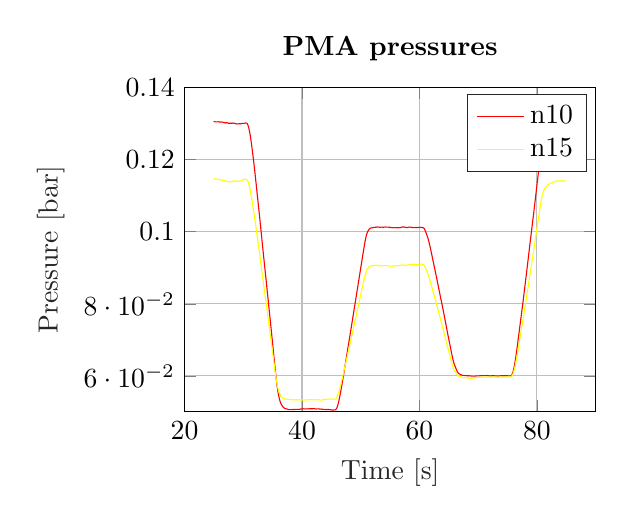
\begin{tikzpicture}

\begin{axis}[%
width=2.0556in,
height=1.62135in,
at={(1.011in,0.642in)},
scale only axis,
xmin=20,
xmax=90,
xlabel style={font=\color{white!15!black}},
xlabel={Time [s]},
ymin=0.05,
ymax=0.14,
ylabel style={font=\color{white!15!black}},
ylabel={Pressure [bar]},
axis background/.style={fill=white},
title style={font=\bfseries},
title={PMA pressures},
xmajorgrids,
ymajorgrids,
legend style={legend cell align=left, align=left, draw=white!15!black}
]
\addplot [color=red]
  table[row sep=crcr]{%
24.95	0.130615982404692\\
25	0.130593362658847\\
25.05	0.130580312805474\\
25.1	0.130582922776149\\
25.15	0.130553343108504\\
25.2	0.130505493646139\\
25.25	0.130492443792766\\
25.3	0.130497663734115\\
25.35	0.13049853372434\\
25.4	0.130501143695015\\
25.45	0.130503753665689\\
25.5	0.130502883675464\\
25.55	0.130501143695015\\
25.6	0.130507233626588\\
25.65	0.130507233626588\\
25.7	0.13050027370479\\
25.75	0.130508103616813\\
25.8	0.130522893450635\\
25.85	0.130510713587488\\
25.9	0.130485483870968\\
25.95	0.130467214076246\\
26	0.130455904203324\\
26.05	0.130455034213099\\
26.1	0.130450684261975\\
26.15	0.130437634408602\\
26.2	0.130441984359726\\
26.25	0.130455904203324\\
26.3	0.130450684261975\\
26.35	0.130432414467253\\
26.4	0.130421974584555\\
26.45	0.130416754643206\\
26.5	0.130406314760508\\
26.55	0.130379345063538\\
26.6	0.130348895405669\\
26.65	0.130340195503421\\
26.7	0.130323665689149\\
26.75	0.130284516129032\\
26.8	0.13026972629521\\
26.85	0.130267116324535\\
26.9	0.130228836754643\\
26.95	0.13019403714565\\
27	0.130206217008797\\
27.05	0.130238406647116\\
27.1	0.130260156402737\\
27.15	0.130267116324535\\
27.2	0.130251456500488\\
27.25	0.130227966764418\\
27.3	0.130202737047898\\
27.35	0.130164457478006\\
27.4	0.130135747800586\\
27.45	0.130126177908113\\
27.5	0.130119217986314\\
27.55	0.130119217986314\\
27.6	0.130128787878787\\
27.65	0.130134007820136\\
27.7	0.130122697947214\\
27.75	0.130106168132942\\
27.8	0.130100078201368\\
27.85	0.13011834799609\\
27.9	0.130134877810361\\
27.95	0.130120957966764\\
28	0.130115738025415\\
28.05	0.130122697947214\\
28.1	0.130122697947214\\
28.15	0.130126177908113\\
28.2	0.130147927663734\\
28.25	0.130173157380254\\
28.3	0.130160977517106\\
28.35	0.130143577712609\\
28.4	0.130142707722384\\
28.45	0.130124437927663\\
28.5	0.130103558162267\\
28.55	0.130082678396871\\
28.6	0.130041788856304\\
28.65	0.130002639296187\\
28.7	0.12998871945259\\
28.75	0.12998871945259\\
28.8	0.129970449657868\\
28.85	0.129943479960899\\
28.9	0.129927820136852\\
28.95	0.129927820136852\\
29	0.129926950146627\\
29.05	0.129918250244379\\
29.1	0.129927820136852\\
29.15	0.1299365200391\\
29.2	0.129940869990224\\
29.25	0.129952179863147\\
29.3	0.129973929618768\\
29.35	0.129982629521016\\
29.4	0.129971319648093\\
29.45	0.129979149560116\\
29.5	0.129982629521015\\
29.55	0.129969579667643\\
29.6	0.129967839687193\\
29.65	0.12998523949169\\
29.7	0.13001220918866\\
29.75	0.130049618768328\\
29.8	0.130073108504398\\
29.85	0.130069628543499\\
29.9	0.130065278592375\\
29.95	0.130072238514173\\
30	0.130087028347996\\
30.05	0.130083548387096\\
30.1	0.130074848484848\\
30.15	0.130094858260019\\
30.2	0.130125307917888\\
30.25	0.130135747800586\\
30.3	0.130155757575757\\
30.35	0.130189687194525\\
30.4	0.13019055718475\\
30.45	0.130164457478006\\
30.5	0.130154887585532\\
30.55	0.130146187683284\\
30.6	0.130113998044966\\
30.65	0.130053968719452\\
30.7	0.129930430107527\\
30.75	0.129752082111437\\
30.8	0.129544154447703\\
30.85	0.129293597262952\\
30.9	0.129003020527859\\
30.95	0.128679384164223\\
31	0.12831137829912\\
31.05	0.127919882697947\\
31.1	0.127513597262952\\
31.15	0.127080342130987\\
31.2	0.126600977517107\\
31.25	0.126065933528837\\
31.3	0.125501309872923\\
31.35	0.124921026392962\\
31.4	0.124312903225807\\
31.45	0.123680420332356\\
31.5	0.123040977517107\\
31.55	0.122401534701858\\
31.6	0.121769921798632\\
31.65	0.12111916911046\\
31.7	0.120437096774194\\
31.75	0.119748934506354\\
31.8	0.119035542521994\\
31.85	0.118315190615836\\
31.9	0.117613978494624\\
31.95	0.116901456500489\\
32	0.116156744868035\\
32.05	0.115394633431085\\
32.1	0.114629042033235\\
32.15	0.113860840664711\\
32.2	0.113102209188661\\
32.25	0.112337487781036\\
32.3	0.111558846529814\\
32.35	0.11079064516129\\
32.4	0.110025923753665\\
32.45	0.109258592375366\\
32.5	0.108488651026393\\
32.55	0.107705659824047\\
32.6	0.10692440860215\\
32.65	0.106145767350928\\
32.7	0.105359296187683\\
32.75	0.104575434995112\\
32.8	0.10379679374389\\
32.85	0.103004232649071\\
32.9	0.102201231671554\\
32.95	0.101419110459433\\
33	0.100633509286412\\
33.05	0.0998226783968715\\
33.1	0.0990083675464315\\
33.15	0.0981940566959917\\
33.2	0.097374525904203\\
33.25	0.0965523851417396\\
33.3	0.0957511241446722\\
33.35	0.0949742228739\\
33.4	0.0941860117302051\\
33.45	0.093388230694037\\
33.5	0.0925991495601171\\
33.55	0.0918074584555227\\
33.6	0.091022727272727\\
33.65	0.0902493059628541\\
33.7	0.0894732746823068\\
33.75	0.0886955034213098\\
33.8	0.0879203421309872\\
33.85	0.0871460508308894\\
33.9	0.0863665395894426\\
33.95	0.0855713685239489\\
34	0.0847831573802539\\
34.05	0.084009736070381\\
34.1	0.0832206549364611\\
34.15	0.0824307038123164\\
34.2	0.0816433626588463\\
34.25	0.0808455816226781\\
34.3	0.0800382306940369\\
34.35	0.0792308797653957\\
34.4	0.0784417986314759\\
34.45	0.0776579374389051\\
34.5	0.0768732062561094\\
34.55	0.0760823851417397\\
34.6	0.0752837341153468\\
34.65	0.0744894330400779\\
34.7	0.0736873020527854\\
34.75	0.0728773411534697\\
34.8	0.0720813000977511\\
34.85	0.0712817790811332\\
34.9	0.0704657282502437\\
34.95	0.0696435874877801\\
35	0.068824926686216\\
35.05	0.0680140957966755\\
35.1	0.0672137047898328\\
35.15	0.0664228836754631\\
35.2	0.0656251026392949\\
35.25	0.0648151417399793\\
35.3	0.0639938709677409\\
35.35	0.0631786901270761\\
35.4	0.0623748191593339\\
35.45	0.0615892179863133\\
35.5	0.060807096774192\\
35.55	0.060023235581621\\
35.6	0.0592663440860198\\
35.65	0.0585442521994118\\
35.7	0.0578656598240453\\
35.75	0.0572253470185713\\
35.8	0.0566154838709661\\
35.85	0.056071739980448\\
35.9	0.0555871554252182\\
35.95	0.0551312805474078\\
36	0.05471368523949\\
36.05	0.054327409579666\\
36.1	0.0539602737047881\\
36.15	0.0536157575757557\\
36.2	0.0533016911045923\\
36.25	0.0530198142717477\\
36.3	0.0527796969696949\\
36.35	0.0525665493646118\\
36.4	0.05237167155425\\
36.45	0.0522020234604083\\
36.5	0.0520506451612881\\
36.55	0.0519079667644162\\
36.6	0.0517626783968696\\
36.65	0.05163304985337\\
36.7	0.0515303910068401\\
36.75	0.0514407820136826\\
36.8	0.0513572629520992\\
36.85	0.0512685239491667\\
36.9	0.0511797849462342\\
36.95	0.0511067057673486\\
37	0.0510562463343085\\
37.05	0.0510170967741912\\
37.1	0.0509762072336242\\
37.15	0.0509405376344061\\
37.2	0.0509144379276611\\
37.25	0.0508857282502417\\
37.3	0.0508596285434967\\
37.35	0.0508396187683255\\
37.4	0.0508196089931543\\
37.45	0.0507961192570837\\
37.5	0.0507674095796643\\
37.55	0.0507439198435939\\
37.6	0.0507213000977483\\
37.65	0.0506960703812283\\
37.7	0.0506708406647082\\
37.75	0.0506543108504365\\
37.8	0.0506438709677386\\
37.85	0.0506316911045909\\
37.9	0.0506273411534666\\
37.95	0.0506195112414431\\
38	0.0506134213098695\\
38.05	0.0506203812316684\\
38.1	0.0506256011730175\\
38.15	0.0506334310850408\\
38.2	0.0506490909090875\\
38.25	0.0506630107526847\\
38.3	0.0506734506353828\\
38.35	0.0506638807429097\\
38.4	0.0506490909090875\\
38.45	0.0506499608993124\\
38.5	0.0506517008797623\\
38.55	0.0506577908113362\\
38.6	0.0506621407624605\\
38.65	0.0506630107526853\\
38.7	0.0506647507331348\\
38.75	0.0506630107526851\\
38.8	0.0506691006842589\\
38.85	0.0506830205278561\\
38.9	0.050693460410554\\
38.95	0.0507091202346009\\
39	0.0507186901270741\\
39.05	0.0507134701857252\\
39.1	0.0507143401759501\\
39.15	0.0507169501466246\\
39.2	0.0507143401759501\\
39.25	0.0507134701857254\\
39.3	0.0507082502443764\\
39.35	0.050704770283477\\
39.4	0.0507030303030273\\
39.45	0.0507012903225776\\
39.5	0.0507073802541516\\
39.55	0.0507195601172993\\
39.6	0.0507317399804469\\
39.65	0.0507465298142691\\
39.7	0.0507717595307893\\
39.75	0.050794379276635\\
39.8	0.0508004692082087\\
39.85	0.0508126490713563\\
39.9	0.050834398826977\\
39.95	0.0508517986314736\\
40	0.0508587585532723\\
40.05	0.0508578885630476\\
40.1	0.0508552785923731\\
40.15	0.0508535386119236\\
40.2	0.0508596285434976\\
40.25	0.0508613685239473\\
40.3	0.0508552785923733\\
40.35	0.0508404887585511\\
40.4	0.0508274389051788\\
40.45	0.0508204789833803\\
40.5	0.0508117790811321\\
40.55	0.050812649071357\\
40.6	0.0508213489736054\\
40.65	0.0508265689149544\\
40.7	0.0508326588465282\\
40.75	0.0508326588465282\\
40.8	0.0508343988269779\\
40.85	0.0508396187683267\\
40.9	0.0508422287390012\\
40.95	0.0508570185728233\\
41	0.0508657184750717\\
41.05	0.050859628543498\\
41.1	0.0508526686216992\\
41.15	0.0508483186705751\\
41.2	0.0508509286412497\\
41.25	0.0508570185728237\\
41.3	0.0508657184750721\\
41.35	0.0508805083088941\\
41.4	0.0508918181818169\\
41.45	0.0508874682306928\\
41.5	0.0508744183773203\\
41.55	0.0508674584555218\\
41.6	0.050872678396871\\
41.65	0.0508778983382202\\
41.7	0.0508813782991197\\
41.75	0.0508839882697943\\
41.8	0.0508822482893447\\
41.85	0.0508900782013681\\
41.9	0.0509031280547404\\
41.95	0.050909217986314\\
42	0.0509013880742906\\
42.05	0.0508900782013679\\
42.1	0.050880508308895\\
42.15	0.0508639784946233\\
42.2	0.050845708699902\\
42.25	0.0508343988269793\\
42.3	0.0508248289345064\\
42.35	0.0508187390029327\\
42.4	0.0508152590420336\\
42.45	0.0508161290322585\\
42.5	0.0508274389051813\\
42.55	0.0508317888563054\\
42.6	0.0508309188660805\\
42.65	0.0508300488758556\\
42.7	0.0508317888563052\\
42.75	0.05083265884653\\
42.8	0.050827438905181\\
42.85	0.0508222189638321\\
42.9	0.0508152590420336\\
42.95	0.0508100391006845\\
43	0.0508074291300099\\
43.05	0.0508004692082112\\
43.1	0.0507961192570871\\
43.15	0.0507874193548389\\
43.2	0.0507700195503423\\
43.25	0.0507526197458457\\
43.3	0.0507369599217988\\
43.35	0.0507343499511244\\
43.4	0.0507404398826981\\
43.45	0.0507413098729229\\
43.5	0.0507343499511242\\
43.55	0.0507239100684261\\
43.6	0.0507117302052784\\
43.65	0.0506978103616811\\
43.7	0.0506917204301073\\
43.75	0.0506917204301072\\
43.8	0.0506812805474091\\
43.85	0.0506612707722381\\
43.9	0.0506412609970672\\
43.95	0.0506299511241446\\
44	0.0506247311827956\\
44.05	0.0506325610948188\\
44.1	0.0506456109481912\\
44.15	0.0506508308895402\\
44.2	0.0506543108504395\\
44.25	0.0506551808406643\\
44.3	0.050656050830889\\
44.35	0.0506543108504394\\
44.4	0.0506604007820132\\
44.45	0.0506691006842614\\
44.5	0.0506682306940364\\
44.55	0.0506595307917882\\
44.6	0.0506499608993153\\
44.65	0.0506377810361677\\
44.7	0.0506247311827952\\
44.75	0.0506151612903221\\
44.8	0.0506125513196476\\
44.85	0.0506055913978491\\
44.9	0.0505847116324533\\
44.95	0.0505612218963831\\
45	0.0505499120234605\\
45.05	0.0505455620723364\\
45.1	0.0505368621700882\\
45.15	0.0505351221896385\\
45.2	0.0505325122189639\\
45.25	0.0505333822091886\\
45.3	0.0505325122189639\\
45.35	0.0505264222873903\\
45.4	0.0505316422287393\\
45.45	0.0505394721407628\\
45.5	0.0505490420332359\\
45.55	0.0505655718475076\\
45.6	0.0505760117302055\\
45.65	0.050588191593353\\
45.7	0.0506212512218966\\
45.75	0.0506830205278595\\
45.8	0.0507708895405672\\
45.85	0.0508805083088957\\
45.9	0.051020576735093\\
45.95	0.0511919648093842\\
46	0.0513938025415445\\
46.05	0.0516313098729228\\
46.1	0.0519123167155426\\
46.15	0.0522237732160315\\
46.2	0.0525517595307919\\
46.25	0.052896275659824\\
46.3	0.0532529716520038\\
46.35	0.0536348973607037\\
46.4	0.0540307429130008\\
46.45	0.0544387683284457\\
46.5	0.0548737634408603\\
46.55	0.0553209384164223\\
46.6	0.0557611534701856\\
46.65	0.0562178983382207\\
46.7	0.0566876930596282\\
46.75	0.0571444379276633\\
46.8	0.0576151026392958\\
46.85	0.0580988172043007\\
46.9	0.0585764418377318\\
46.95	0.0590618963831865\\
47	0.059553440860215\\
47.05	0.0600362854349951\\
47.1	0.0605304398826979\\
47.15	0.0610350342130985\\
47.2	0.0615378885630495\\
47.25	0.0620485728250239\\
47.3	0.0625583870967736\\
47.35	0.0630629814271742\\
47.4	0.0635727956989239\\
47.45	0.064070430107526\\
47.5	0.0645680645161281\\
47.55	0.0650700488758545\\
47.6	0.0655642033235576\\
47.65	0.0660635777126096\\
47.7	0.0665646920821111\\
47.75	0.0670640664711629\\
47.8	0.0675608308895402\\
47.85	0.0680671652003907\\
47.9	0.0685752394916909\\
47.95	0.0690833137829911\\
48	0.0695826881720429\\
48.05	0.0700751026392959\\
48.1	0.0705779569892469\\
48.15	0.0710929912023456\\
48.2	0.0716080254154445\\
48.25	0.0721126197458453\\
48.3	0.0726146041055715\\
48.35	0.0731078885630495\\
48.4	0.0736037829912021\\
48.45	0.0741144672531767\\
48.5	0.0746399413489733\\
48.55	0.0751541055718473\\
48.6	0.0756560899315737\\
48.65	0.0761711241446724\\
48.7	0.0766800684261973\\
48.75	0.0771837927663734\\
48.8	0.0777005669599218\\
48.85	0.0782277810361681\\
48.9	0.0787523851417399\\
48.95	0.0792543695014661\\
49	0.0797476539589441\\
49.05	0.0802487683284458\\
49.1	0.0807507526881722\\
49.15	0.0812570869990225\\
49.2	0.0817703812316713\\
49.25	0.0822819354838707\\
49.3	0.0828004496578688\\
49.35	0.0833233137829909\\
49.4	0.0838279081133917\\
49.45	0.0843290224828934\\
49.5	0.0848414467253177\\
49.55	0.0853617008797652\\
49.6	0.0858697751710652\\
49.65	0.0863743695014659\\
49.7	0.086892013685239\\
49.75	0.0874044379276633\\
49.8	0.0879125122189635\\
49.85	0.0884301564027366\\
49.9	0.0889495405669594\\
49.95	0.0894697947214071\\
50	0.0899917888563044\\
50.05	0.0905016031280541\\
50.1	0.0910070674486796\\
50.15	0.0915064418377314\\
50.2	0.0919953763440853\\
50.25	0.0925025806451606\\
50.3	0.0930280547409572\\
50.35	0.0935578787878779\\
50.4	0.0940781329423256\\
50.45	0.0945835972629514\\
50.5	0.0950725317693053\\
50.55	0.095552766373411\\
50.6	0.0960477908113386\\
50.65	0.0965375953079173\\
50.7	0.0970065200391\\
50.75	0.0974432551319639\\
50.8	0.0978373607038114\\
50.85	0.0982210263929609\\
50.9	0.098596862170087\\
50.95	0.0989178885630489\\
51	0.099206725317692\\
51.05	0.099491212121211\\
51.1	0.0997304594330389\\
51.15	0.0999235972629508\\
51.2	0.10008193548387\\
51.25	0.100224613880742\\
51.3	0.100372512218963\\
51.35	0.100501270772238\\
51.4	0.100631769305962\\
51.45	0.100753567937438\\
51.5	0.100839696969696\\
51.55	0.100897116324535\\
51.6	0.100949315738024\\
51.65	0.101002385141739\\
51.7	0.101034574780058\\
51.75	0.101063284457477\\
51.8	0.101082424242423\\
51.85	0.101086774193548\\
51.9	0.101098954056695\\
51.95	0.101104173998044\\
52	0.101116353861192\\
52.05	0.101146803519061\\
52.1	0.101156373411534\\
52.15	0.10117551319648\\
52.2	0.101215532746822\\
52.25	0.101223362658846\\
52.3	0.101212922776148\\
52.35	0.1012042228739\\
52.4	0.1012042228739\\
52.45	0.10122945259042\\
52.5	0.101243372434018\\
52.55	0.101247722385142\\
52.6	0.101261642228739\\
52.65	0.101283391984359\\
52.7	0.10130514173998\\
52.75	0.101314711632453\\
52.8	0.101331241446725\\
52.85	0.101340811339198\\
52.9	0.101332981427174\\
52.95	0.101311231671554\\
53	0.101293831867057\\
53.05	0.101299051808406\\
53.1	0.101288611925708\\
53.15	0.101259032258064\\
53.2	0.101247722385141\\
53.25	0.101248592375366\\
53.3	0.101251202346041\\
53.35	0.101264252199413\\
53.4	0.101273822091887\\
53.45	0.101274692082112\\
53.5	0.101272082111437\\
53.55	0.101272952101662\\
53.6	0.101278172043011\\
53.65	0.101269472140763\\
53.7	0.101265122189638\\
53.75	0.101268602150538\\
53.8	0.10125816226784\\
53.85	0.101245982404692\\
53.9	0.101252942326491\\
53.95	0.101272952101662\\
54	0.101290351906158\\
54.05	0.101291221896383\\
54.1	0.101299921798631\\
54.15	0.101312101661779\\
54.2	0.101309491691105\\
54.25	0.101309491691105\\
54.3	0.101299921798632\\
54.35	0.101277302052787\\
54.4	0.101274692082112\\
54.45	0.101293831867058\\
54.5	0.101292091886609\\
54.55	0.10128339198436\\
54.6	0.101295571847508\\
54.65	0.101299051808407\\
54.7	0.101282521994136\\
54.75	0.101266862170089\\
54.8	0.101259032258065\\
54.85	0.101257292277615\\
54.9	0.101249462365592\\
54.95	0.101228582600196\\
55	0.101201612903226\\
55.05	0.101186823069404\\
55.1	0.101178993157381\\
55.15	0.101170293255133\\
55.2	0.101166813294233\\
55.25	0.101152893450636\\
55.3	0.101143323558163\\
55.35	0.101141583577713\\
55.4	0.101131143695015\\
55.45	0.101118963831867\\
55.5	0.101125053763441\\
55.55	0.101137233626589\\
55.6	0.101140713587488\\
55.65	0.101136363636364\\
55.7	0.101133753665689\\
55.75	0.101143323558162\\
55.8	0.10115550342131\\
55.85	0.10115898338221\\
55.9	0.101152893450636\\
55.95	0.10115898338221\\
56	0.101148543499512\\
56.05	0.101117223851419\\
56.1	0.101105043988271\\
56.15	0.101104173998046\\
56.2	0.101119833822093\\
56.25	0.101146803519063\\
56.3	0.101154633431086\\
56.35	0.101148543499512\\
56.4	0.101130273704791\\
56.45	0.101118093841643\\
56.5	0.101125923753667\\
56.55	0.101141583577714\\
56.6	0.101155503421311\\
56.65	0.101159853372435\\
56.7	0.101168553274683\\
56.75	0.101178123167156\\
56.8	0.101193782991203\\
56.85	0.101222492668622\\
56.9	0.101243372434018\\
56.95	0.101272952101662\\
57	0.101290351906159\\
57.05	0.101298181818182\\
57.1	0.101336461388075\\
57.15	0.101344291300099\\
57.2	0.101316451612904\\
57.25	0.101314711632454\\
57.3	0.101320801564028\\
57.35	0.101325151515152\\
57.4	0.101322541544478\\
57.45	0.101297311827958\\
57.5	0.101271212121213\\
57.55	0.10125990224829\\
57.6	0.101251202346042\\
57.65	0.101233802541545\\
57.7	0.101217272727273\\
57.75	0.1012077028348\\
57.8	0.101192043010753\\
57.85	0.101177253176931\\
57.9	0.101180733137831\\
57.95	0.101190303030304\\
58	0.101208572825025\\
58.05	0.101228582600196\\
58.1	0.101250332355817\\
58.15	0.101284261974585\\
58.2	0.101305141739981\\
58.25	0.101306011730206\\
58.3	0.101288611925709\\
58.35	0.101276432062561\\
58.4	0.101279912023461\\
58.45	0.101266862170088\\
58.5	0.101246852394917\\
58.55	0.101245982404692\\
58.6	0.101243372434018\\
58.65	0.101226842619746\\
58.7	0.1012042228739\\
58.75	0.101179863147605\\
58.8	0.101178993157381\\
58.85	0.101186823069404\\
58.9	0.101172033235582\\
58.95	0.101146803519062\\
59	0.101138973607038\\
59.05	0.101148543499511\\
59.1	0.101145933528837\\
59.15	0.101143323558162\\
59.2	0.101146803519062\\
59.25	0.101157243401759\\
59.3	0.101184213098729\\
59.35	0.101214662756598\\
59.4	0.101222492668621\\
59.45	0.101197262952101\\
59.5	0.101182473118279\\
59.55	0.101185083088954\\
59.6	0.101182473118279\\
59.65	0.101181603128054\\
59.7	0.101184213098729\\
59.75	0.101199002932551\\
59.8	0.101211182795699\\
59.85	0.101195522971652\\
59.9	0.101195522971652\\
59.95	0.101211182795699\\
60	0.101215532746823\\
60.05	0.101212922776148\\
60.1	0.101212052785923\\
60.15	0.101225102639296\\
60.2	0.101236412512218\\
60.25	0.101241632453568\\
60.3	0.101225102639296\\
60.35	0.101192043010752\\
60.4	0.10118073313783\\
60.45	0.101185953079179\\
60.5	0.101178123167155\\
60.55	0.101152893450635\\
60.6	0.101113743890518\\
60.65	0.101079814271749\\
60.7	0.101043274682307\\
60.75	0.100971065493646\\
60.8	0.100869276637341\\
60.85	0.100737908113391\\
60.9	0.100570869990224\\
60.95	0.100385562072336\\
61	0.100199384164222\\
61.05	0.0999958064516118\\
61.1	0.0997765689149549\\
61.15	0.0995590713587479\\
61.2	0.0993293939393933\\
61.25	0.0990944965786895\\
61.3	0.0988787390029318\\
61.35	0.0986612414467246\\
61.4	0.0984167741935478\\
61.45	0.0981488172043006\\
61.5	0.0978556304985332\\
61.55	0.0975537438905176\\
61.6	0.0972431573802538\\
61.65	0.0969082111436947\\
61.7	0.0965671749755618\\
61.75	0.0962287487781033\\
61.8	0.0958720527859233\\
61.85	0.0954996969696966\\
61.9	0.0951299511241444\\
61.95	0.0947575953079177\\
62	0.0943826295210165\\
62.05	0.0939937438905181\\
62.1	0.0935874584555229\\
62.15	0.0931959628543497\\
62.2	0.0928157771260993\\
62.25	0.0924303714564999\\
62.3	0.0920501857282496\\
62.35	0.0916673900293247\\
62.4	0.0912732844574773\\
62.45	0.0908774389051804\\
62.5	0.090487683284457\\
62.55	0.0900996676441833\\
62.6	0.0897073020527856\\
62.65	0.0893114565004884\\
62.7	0.0889130009775169\\
62.75	0.0885128054740957\\
62.8	0.088119569892473\\
62.85	0.0877350342130985\\
62.9	0.0873400586510261\\
62.95	0.086943343108504\\
63	0.0865431476050826\\
63.05	0.0861238123167151\\
63.1	0.0857175268817201\\
63.15	0.0853155913978492\\
63.2	0.0849040860215052\\
63.25	0.0845038905180838\\
63.3	0.0841184848484845\\
63.35	0.0837226392961874\\
63.4	0.0833085239491688\\
63.45	0.0829039784946232\\
63.5	0.082503782991202\\
63.55	0.0820905376344085\\
63.6	0.0816920821114369\\
63.65	0.0813127663734114\\
63.7	0.0809317106549363\\
63.75	0.0805497849462364\\
63.8	0.0801521994134896\\
63.85	0.079744173998045\\
63.9	0.0793378885630499\\
63.95	0.0789403030303031\\
64	0.0785305376344088\\
64.05	0.0781051124144675\\
64.1	0.0776831671554255\\
64.15	0.0772620918866085\\
64.2	0.0768505865102645\\
64.25	0.0764303812316721\\
64.3	0.0759884261974591\\
64.35	0.0755456011730214\\
64.4	0.075115826001956\\
64.45	0.0747078005865111\\
64.5	0.0743015151515159\\
64.55	0.0738726099706753\\
64.6	0.0734367448680361\\
64.65	0.0730087096774204\\
64.7	0.0725902443792776\\
64.75	0.0721674291300108\\
64.8	0.0717411339198446\\
64.85	0.0713296285435003\\
64.9	0.0709181231671563\\
64.95	0.0705066177908122\\
65	0.0701055522971661\\
65.05	0.0697070967741945\\
65.1	0.0693112512218974\\
65.15	0.0689075757575768\\
65.2	0.0685030303030313\\
65.25	0.0680923949169118\\
65.3	0.0676878494623663\\
65.35	0.0672946138807438\\
65.4	0.0668865884652993\\
65.45	0.0664750830889554\\
65.5	0.066066187683286\\
65.55	0.0656642521994151\\
65.6	0.0652805865102655\\
65.65	0.064907360703814\\
65.7	0.0645437047898357\\
65.75	0.0642070185728269\\
65.8	0.0639025219941367\\
65.85	0.0636223851417418\\
65.9	0.0633648680351925\\
65.95	0.0631273607038143\\
66	0.0629072531769326\\
66.05	0.0627054154447725\\
66.1	0.0625053176930619\\
66.15	0.0623026099706767\\
66.2	0.0621086021505398\\
66.25	0.0619111143695037\\
66.3	0.0616979667644205\\
66.35	0.0614943890518106\\
66.4	0.061314301075271\\
66.45	0.0611524828934527\\
66.5	0.06101328445748\\
66.55	0.0608871358748797\\
66.6	0.060778387096776\\
66.65	0.0607000879765414\\
66.7	0.0606339687194545\\
66.75	0.0605730694037165\\
66.8	0.060525219941351\\
66.85	0.0604869403714586\\
66.9	0.0604504007820157\\
66.95	0.0604008113392005\\
67	0.0603503519061604\\
67.05	0.0603129423264926\\
67.1	0.0602798826979491\\
67.15	0.0602503030303049\\
67.2	0.0602163734115367\\
67.25	0.0601833137829933\\
67.3	0.0601624340175976\\
67.35	0.0601432942326513\\
67.4	0.0601285043988291\\
67.45	0.0601258944281545\\
67.5	0.0601215444770304\\
67.55	0.0601102346041078\\
67.6	0.0601058846529837\\
67.65	0.0600963147605105\\
67.7	0.0600797849462387\\
67.75	0.060071955034215\\
67.8	0.0600693450635404\\
67.85	0.0600658651026411\\
67.9	0.0600597751710673\\
67.95	0.060061515151517\\
68	0.060066735092866\\
68.05	0.0600615151515171\\
68.1	0.0600449853372455\\
68.15	0.0600267155425241\\
68.2	0.0600154056696015\\
68.25	0.0600214956011755\\
68.3	0.0600319354838733\\
68.35	0.060033675464323\\
68.4	0.0600336754643232\\
68.45	0.0600258455522997\\
68.5	0.060018885630501\\
68.55	0.0600180156402761\\
68.6	0.0600093157380277\\
68.65	0.0599936559139808\\
68.7	0.0599823460410581\\
68.75	0.0599710361681355\\
68.8	0.0599527663734142\\
68.85	0.0599327565982431\\
68.9	0.0599257966764446\\
68.95	0.0599179667644213\\
69	0.0599136168132972\\
69.05	0.059919706744871\\
69.1	0.0599179667644213\\
69.15	0.0599179667644211\\
69.2	0.0599179667644211\\
69.25	0.0599153567937467\\
69.3	0.0599257966764446\\
69.35	0.0599423264907163\\
69.4	0.0599466764418402\\
69.45	0.0599405865102664\\
69.5	0.0599397165200417\\
69.55	0.0599553763440886\\
69.6	0.0599727761485852\\
69.65	0.0599875659824074\\
69.7	0.0599927859237564\\
69.75	0.059989305962857\\
69.8	0.0599927859237564\\
69.85	0.0599971358748807\\
69.9	0.0599997458455553\\
69.95	0.0599971358748808\\
70	0.0599893059628574\\
70.05	0.0599901759530821\\
70.1	0.060001485826005\\
70.15	0.0600110557184781\\
70.2	0.0600197556207265\\
70.25	0.0600371554252233\\
70.3	0.060043245356797\\
70.35	0.0600432453567969\\
70.4	0.0600458553274711\\
70.45	0.0600441153470213\\
70.5	0.0600562952101688\\
70.55	0.0600789149560145\\
70.6	0.0600937047898366\\
70.65	0.0600937047898366\\
70.7	0.060085874877813\\
70.75	0.0600832649071384\\
70.8	0.0600884848484874\\
70.85	0.0600867448680377\\
70.9	0.0600832649071384\\
70.95	0.0600823949169136\\
71	0.0600815249266889\\
71.05	0.0600789149560143\\
71.1	0.0600728250244403\\
71.15	0.0600710850439906\\
71.2	0.060069345063541\\
71.25	0.0600632551319672\\
71.3	0.0600632551319672\\
71.35	0.0600702150537657\\
71.4	0.0600815249266883\\
71.45	0.0600971847507353\\
71.5	0.0601119745845574\\
71.55	0.0601198044965809\\
71.6	0.060109364613883\\
71.65	0.0600884848484872\\
71.7	0.0600676050830913\\
71.75	0.0600458553274704\\
71.8	0.0600293255131986\\
71.85	0.0600136656891515\\
71.9	0.0600023558162286\\
71.95	0.0600049657869032\\
72	0.060011925708702\\
72.05	0.0600154056696013\\
72.1	0.060011925708702\\
72.15	0.0600093157380275\\
72.2	0.0600171456500512\\
72.25	0.060023235581625\\
72.3	0.0600249755620746\\
72.35	0.0600258455522996\\
72.4	0.0600249755620746\\
72.45	0.0600293255131987\\
72.5	0.0600301955034235\\
72.55	0.0600284555229736\\
72.6	0.0600328054740976\\
72.65	0.0600362854349967\\
72.7	0.0600362854349967\\
72.75	0.0600310654936479\\
72.8	0.0600180156402756\\
72.85	0.0600084457478024\\
72.9	0.0600084457478024\\
72.95	0.0600014858260039\\
73	0.0599884359726314\\
73.05	0.059989305962856\\
73.1	0.0599901759530807\\
73.15	0.059989305962856\\
73.2	0.0599901759530807\\
73.25	0.0599771260997082\\
73.3	0.0599597262952116\\
73.35	0.0599458064516142\\
73.4	0.0599431964809396\\
73.45	0.0599562463343121\\
73.5	0.0599614662756611\\
73.55	0.0599701661779095\\
73.6	0.0599893059628558\\
73.65	0.0599988758553288\\
73.7	0.0600040957966776\\
73.75	0.0600127956989258\\
73.8	0.060021495601174\\
73.85	0.0600293255131975\\
73.9	0.0600319354838719\\
73.95	0.0600345454545462\\
74	0.0600415053763447\\
74.05	0.0600449853372441\\
74.1	0.0600449853372441\\
74.15	0.0600397653958952\\
74.2	0.0600293255131973\\
74.25	0.0600241055718483\\
74.3	0.0600214956011737\\
74.35	0.060014535679375\\
74.4	0.0600223655913986\\
74.45	0.0600371554252208\\
74.5	0.0600397653958952\\
74.55	0.0600293255131973\\
74.6	0.0600232355816235\\
74.65	0.0600232355816233\\
74.7	0.0600354154447709\\
74.75	0.0600493352883682\\
74.8	0.060049335288368\\
74.85	0.0600441153470188\\
74.9	0.0600301955034213\\
74.95	0.060021495601173\\
75	0.0600223655913977\\
75.05	0.0600232355816226\\
75.1	0.0600110557184751\\
75.15	0.0599962658846529\\
75.2	0.0599884359726293\\
75.25	0.0599814760508306\\
75.3	0.0599806060606058\\
75.35	0.0599797360703811\\
75.4	0.0599866959921798\\
75.45	0.0600023558162267\\
75.5	0.0600084457478005\\
75.55	0.0600232355816225\\
75.6	0.0600562952101658\\
75.65	0.0601128445747797\\
75.7	0.0602007135874876\\
75.75	0.0603294721407623\\
75.8	0.0604991202346039\\
75.85	0.060712267839687\\
75.9	0.0609697849462362\\
75.95	0.0612507917888557\\
76	0.0615552883675456\\
76.05	0.0618902346041047\\
76.1	0.0622747702834792\\
76.15	0.0626993255131955\\
76.2	0.0631543304007808\\
76.25	0.0636371749755607\\
76.3	0.0641339393939381\\
76.35	0.0646524535679362\\
76.4	0.0651892375366556\\
76.45	0.0657355913978481\\
76.5	0.066291515151514\\
76.55	0.0668752785923743\\
76.6	0.0675008015640263\\
76.65	0.068131544477027\\
76.7	0.0687527174975548\\
76.75	0.0693965102639284\\
76.8	0.0700446529814261\\
76.85	0.0706753958944272\\
76.9	0.0712869990224821\\
76.95	0.0719012121212112\\
77	0.0725458748778093\\
77.05	0.073204457478005\\
77.1	0.073845640273704\\
77.15	0.074480733137829\\
77.2	0.0751175659824035\\
77.25	0.0757500488758542\\
77.3	0.0763912316715532\\
77.35	0.0770315444770274\\
77.4	0.0776735972629513\\
77.45	0.078311300097751\\
77.5	0.0789507429130003\\
77.55	0.0795797458455517\\
77.6	0.0801956989247309\\
77.65	0.0808351417399804\\
77.7	0.0814919843597263\\
77.75	0.0821610068426196\\
77.8	0.0828456891495598\\
77.85	0.083516451612903\\
77.9	0.0841802541544475\\
77.95	0.0848536265884649\\
78	0.0855261290322575\\
78.05	0.0861995014662751\\
78.1	0.0868746138807422\\
78.15	0.0875497262952093\\
78.2	0.0882257086999015\\
78.25	0.0889008211143688\\
78.3	0.0895681036168126\\
78.35	0.0902484359726289\\
78.4	0.0909522580645154\\
78.45	0.0916430303030294\\
78.5	0.0923277126099697\\
78.55	0.0930141348973596\\
78.6	0.0936962072336254\\
78.65	0.0943869794721396\\
78.7	0.0950794916911034\\
78.75	0.095767653958943\\
78.8	0.0964575562072323\\
78.85	0.0971500684261962\\
78.9	0.0978251808406634\\
78.95	0.0984942033235569\\
79	0.0991710557184737\\
79.05	0.0998487781036152\\
79.1	0.100527370478982\\
79.15	0.101209442815247\\
79.2	0.101881075268815\\
79.25	0.10254139784946\\
79.3	0.10320433040078\\
79.35	0.103871612903224\\
79.4	0.104548465298141\\
79.45	0.105221837732159\\
79.5	0.105909130009774\\
79.55	0.10661121212121\\
79.6	0.107302854349949\\
79.65	0.107999716520037\\
79.7	0.108698318670575\\
79.75	0.109397790811338\\
79.8	0.110108572825023\\
79.85	0.110825444770282\\
79.9	0.111529266862169\\
79.95	0.112238308895404\\
80	0.112943870967741\\
80.05	0.113639863147604\\
80.1	0.114352385141738\\
80.15	0.115048377321602\\
80.2	0.115734799608992\\
80.25	0.11642818181818\\
80.3	0.117128523949168\\
80.35	0.117843655913977\\
80.4	0.118545738025414\\
80.45	0.119233030303029\\
80.5	0.119938592375365\\
80.55	0.1206511143695\\
80.6	0.12133753665689\\
80.65	0.12200220918866\\
80.7	0.122639912023459\\
80.75	0.123229765395893\\
80.8	0.123767419354838\\
80.85	0.124257223851416\\
80.9	0.124699178885629\\
80.95	0.125111554252199\\
81	0.125517839687194\\
81.05	0.125901505376344\\
81.1	0.126232101661779\\
81.15	0.126530508308896\\
81.2	0.126797595307918\\
81.25	0.127025532746824\\
81.3	0.127227370478985\\
81.35	0.127402238514175\\
81.4	0.127560576735094\\
81.45	0.12770934506354\\
81.5	0.127843323558163\\
81.55	0.127956422287391\\
81.6	0.128047771260998\\
81.65	0.128127810361682\\
81.7	0.128203499511242\\
81.75	0.128256568914957\\
81.8	0.128305288367547\\
81.85	0.128374887585533\\
81.9	0.128461886608016\\
81.95	0.128519305962855\\
82	0.128536705767351\\
82.05	0.128551495601173\\
82.1	0.128594995112415\\
82.15	0.128656764418378\\
82.2	0.128728103616814\\
82.25	0.128802052785924\\
82.3	0.128857732160313\\
82.35	0.128914281524927\\
82.4	0.128975180840665\\
82.45	0.129032600195504\\
82.5	0.129079579667645\\
82.55	0.129138739002933\\
82.6	0.129202248289345\\
82.65	0.129225738025416\\
82.7	0.129239657869013\\
82.75	0.129264017595308\\
82.8	0.129270977517107\\
82.85	0.129269237536657\\
82.9	0.129273587487782\\
82.95	0.129288377321604\\
83	0.129314477028349\\
83.05	0.12933622678397\\
83.1	0.129350146627567\\
83.15	0.129370156402738\\
83.2	0.129396256109483\\
83.25	0.129412785923755\\
83.3	0.129431055718477\\
83.35	0.129452805474097\\
83.4	0.129441495601175\\
83.45	0.129427575757578\\
83.5	0.129424965786904\\
83.55	0.129413655913981\\
83.6	0.129414525904205\\
83.65	0.129424095796678\\
83.7	0.129427575757578\\
83.75	0.129434535679376\\
83.8	0.129447585532749\\
83.85	0.129451935483873\\
83.9	0.129463245356796\\
83.95	0.129488475073316\\
84	0.129511964809386\\
84.05	0.129534584555232\\
84.1	0.129576344086024\\
84.15	0.129613753665691\\
84.2	0.129650293255134\\
84.25	0.129684222873903\\
84.3	0.129703362658849\\
84.35	0.129739902248292\\
84.4	0.129768611925711\\
84.45	0.12980080156403\\
84.5	0.12982255131965\\
84.55	0.129809501466278\\
84.6	0.129793841642231\\
84.65	0.12977209188661\\
84.7	0.129732942326493\\
84.75	0.129712932551322\\
84.8	0.129699882697949\\
84.85	0.129661603128057\\
84.9	0.129643333333335\\
};
\addlegendentry{n10}

\addplot [color=mycolor1]
  table[row sep=crcr]{%
24.95	0.114646441837733\\
25	0.114640351906159\\
25.05	0.114666451612904\\
25.1	0.114704731182796\\
25.15	0.114702121212122\\
25.2	0.114674281524927\\
25.25	0.114652531769307\\
25.3	0.114629042033236\\
25.35	0.114610772238515\\
25.4	0.114595112414468\\
25.45	0.114593372434018\\
25.5	0.114603812316716\\
25.55	0.114601202346042\\
25.6	0.114593372434018\\
25.65	0.114569012707723\\
25.7	0.114558572825025\\
25.75	0.114564662756599\\
25.8	0.11453421309873\\
25.85	0.114475053763442\\
25.9	0.114424594330402\\
25.95	0.114417634408603\\
26	0.114427204301076\\
26.05	0.114418504398828\\
26.1	0.114396754643207\\
26.15	0.114400234604106\\
26.2	0.114441124144673\\
26.25	0.114437644183774\\
26.3	0.114410674486804\\
26.35	0.114372394916912\\
26.4	0.114318455522972\\
26.45	0.114270606060607\\
26.5	0.114247116324536\\
26.55	0.114222756598241\\
26.6	0.114186217008798\\
26.65	0.114168817204302\\
26.7	0.11415054740958\\
26.75	0.11415402737048\\
26.8	0.114163597262953\\
26.85	0.114172297165201\\
26.9	0.114173167155426\\
26.95	0.114147067448681\\
27	0.114121837732161\\
27.05	0.114086168132943\\
27.1	0.114045278592376\\
27.15	0.114003519061584\\
27.2	0.113950449657869\\
27.25	0.113913040078202\\
27.3	0.113907820136853\\
27.35	0.113915650048876\\
27.4	0.113925219941349\\
27.45	0.1139234799609\\
27.5	0.113893030303031\\
27.55	0.113880850439883\\
27.6	0.113907820136853\\
27.65	0.11389477028348\\
27.7	0.113851270772239\\
27.75	0.113839960899316\\
27.8	0.113850400782014\\
27.85	0.113857360703813\\
27.9	0.113864320625611\\
27.95	0.113883460410557\\
28	0.113911300097752\\
28.05	0.113936529814272\\
28.1	0.113979159335288\\
28.15	0.114033968719453\\
28.2	0.114050498533724\\
28.25	0.114050498533724\\
28.3	0.114069638318671\\
28.35	0.114075728250245\\
28.4	0.11407311827957\\
28.45	0.114085298142718\\
28.5	0.114107917888563\\
28.55	0.114091388074292\\
28.6	0.114037448680352\\
28.65	0.114023528836755\\
28.7	0.114032228739003\\
28.75	0.11402265884653\\
28.8	0.114011348973607\\
28.85	0.114016568914956\\
28.9	0.114017438905181\\
28.95	0.114010478983382\\
29	0.11402091886608\\
29.05	0.114024398826979\\
29.1	0.114016568914956\\
29.15	0.114015698924731\\
29.2	0.114020048875855\\
29.25	0.114012218963831\\
29.3	0.11402091886608\\
29.35	0.114020048875855\\
29.4	0.114010478983382\\
29.45	0.114049628543499\\
29.5	0.114100957966764\\
29.55	0.114140107526881\\
29.6	0.114161857282502\\
29.65	0.114187086999022\\
29.7	0.114214056695992\\
29.75	0.11424798631476\\
29.8	0.114309755620723\\
29.85	0.114391534701857\\
29.9	0.114458523949169\\
29.95	0.114506373411534\\
30	0.11452899315738\\
30.05	0.114508113391984\\
30.1	0.114484623655914\\
30.15	0.114480273704789\\
30.2	0.114497673509286\\
30.25	0.114536823069403\\
30.3	0.114573362658846\\
30.35	0.114588152492668\\
30.4	0.114595982404692\\
30.45	0.114569882697947\\
30.5	0.114538563049853\\
30.55	0.114524643206255\\
30.6	0.114454173998044\\
30.65	0.114338465298142\\
30.7	0.114216666666666\\
30.75	0.114081818181817\\
30.8	0.113920869990224\\
30.85	0.113728602150537\\
30.9	0.113490224828934\\
30.95	0.113189208211143\\
31	0.112862961876832\\
31.05	0.112542805474095\\
31.1	0.112219169110459\\
31.15	0.111842463343108\\
31.2	0.111396158357771\\
31.25	0.110937673509286\\
31.3	0.110452218963831\\
31.35	0.109955454545454\\
31.4	0.1094630400782\\
31.45	0.108978455522971\\
31.5	0.108476471163245\\
31.55	0.107975356793743\\
31.6	0.107500342130986\\
31.65	0.106982697947213\\
31.7	0.106437214076245\\
31.75	0.105902170087976\\
31.8	0.10537147605083\\
31.85	0.10481120234604\\
31.9	0.104246578690126\\
31.95	0.103674125122189\\
32	0.103086011730204\\
32.05	0.102517038123166\\
32.1	0.101949804496578\\
32.15	0.10137735092864\\
32.2	0.100802287390028\\
32.25	0.100215043988269\\
32.3	0.0996104007820128\\
32.35	0.0989883577712601\\
32.4	0.0983697947214068\\
32.45	0.0977703714564997\\
32.5	0.0971822580645153\\
32.55	0.0965819648093833\\
32.6	0.0959599217986305\\
32.65	0.0953604985337234\\
32.7	0.0947810850439874\\
32.75	0.0941677419354829\\
32.8	0.0935448289345055\\
32.85	0.092932355816226\\
32.9	0.0923259726295202\\
32.95	0.0917265493646132\\
33	0.0911166862170082\\
33.05	0.0905155229716515\\
33.1	0.0898891300097747\\
33.15	0.0892305474095793\\
33.2	0.0885919745845549\\
33.25	0.087970801564027\\
33.3	0.0873330987292274\\
33.35	0.0867067057673506\\
33.4	0.0860933626588461\\
33.45	0.0854504398826975\\
33.5	0.0848005571847503\\
33.55	0.0841706842619741\\
33.6	0.0835738709677415\\
33.65	0.0829848875855323\\
33.7	0.0823967741935479\\
33.75	0.0818225806451609\\
33.8	0.0812466471163242\\
33.85	0.0806446138807425\\
33.9	0.0800391006842617\\
33.95	0.0794570772238512\\
34	0.0788611339198433\\
34.05	0.0782443108504396\\
34.1	0.0776126979472139\\
34.15	0.0769950048875853\\
34.2	0.0763990615835775\\
34.25	0.0757874584555228\\
34.3	0.0751584555229714\\
34.35	0.0745390224828932\\
34.4	0.073924809384164\\
34.45	0.0732827565982403\\
34.5	0.0726250439882696\\
34.55	0.0719916911045941\\
34.6	0.0713887878787877\\
34.65	0.0707745747800584\\
34.7	0.0701594916911043\\
34.75	0.0695670283479958\\
34.8	0.0689493352883671\\
34.85	0.0682724828934502\\
34.9	0.0676191202346037\\
34.95	0.0669970772238511\\
35	0.0663724242424239\\
35.05	0.0657677810361679\\
35.1	0.0651587878787877\\
35.15	0.0645558846529813\\
35.2	0.0639460215053761\\
35.25	0.0633187585532744\\
35.3	0.0626967155425218\\
35.35	0.0620833724340175\\
35.4	0.0614813391984359\\
35.45	0.0608975757575756\\
35.5	0.0603146823069402\\
35.55	0.0597265689149559\\
35.6	0.05917238514174\\
35.65	0.0586651808406647\\
35.7	0.0581762463343109\\
35.75	0.0577003616813295\\
35.8	0.057260146627566\\
35.85	0.0568695210166176\\
35.9	0.0565267448680348\\
35.95	0.0562161583577709\\
36	0.0559151417399801\\
36.05	0.0556376148582597\\
36.1	0.0553835777126096\\
36.15	0.0551391104594327\\
36.2	0.0549390127077221\\
36.25	0.0547693646138805\\
36.3	0.0546179863147604\\
36.35	0.0544979276637341\\
36.4	0.0543996187683285\\
36.45	0.0542926099706746\\
36.5	0.0541943010752689\\
36.55	0.0541090420332358\\
36.6	0.0540089931573806\\
36.65	0.0539237341153473\\
36.7	0.0538767546432066\\
36.75	0.0538367350928645\\
36.8	0.0537862756598245\\
36.85	0.0537271163245362\\
36.9	0.0536783968719457\\
36.95	0.0536575171065498\\
37	0.0536488172043016\\
37.05	0.0536270674486809\\
37.1	0.0535879178885636\\
37.15	0.053545288367547\\
37.2	0.0535104887585538\\
37.25	0.0535087487781041\\
37.3	0.0535209286412517\\
37.35	0.0535331085043992\\
37.4	0.0535383284457481\\
37.45	0.0535278885630502\\
37.5	0.0535296285434999\\
37.55	0.0535322385141744\\
37.6	0.0535070087976543\\
37.65	0.0534756891495602\\
37.7	0.0534478494623658\\
37.75	0.0534400195503424\\
37.8	0.0534382795698927\\
37.85	0.0534400195503423\\
37.9	0.0534408895405671\\
37.95	0.0534295796676443\\
38	0.0534165298142719\\
38.05	0.0533991300097752\\
38.1	0.0534078299120234\\
38.15	0.0534243597262951\\
38.2	0.0534374095796675\\
38.25	0.0534365395894428\\
38.3	0.0534226197458454\\
38.35	0.0534034799608991\\
38.4	0.0533756402737046\\
38.45	0.0533625904203323\\
38.5	0.0533599804496578\\
38.55	0.053359110459433\\
38.6	0.0533521505376344\\
38.65	0.053359110459433\\
38.7	0.0533547605083088\\
38.75	0.0533399706744866\\
38.8	0.0533417106549363\\
38.85	0.0533599804496578\\
38.9	0.0533704203323557\\
38.95	0.0533573704789834\\
39	0.0533556304985339\\
39.05	0.0533669403714568\\
39.1	0.0533895601173024\\
39.15	0.0533965200391009\\
39.2	0.053380860215054\\
39.25	0.0533773802541548\\
39.3	0.05337651026393\\
39.35	0.0533704203323562\\
39.4	0.0533591104594334\\
39.45	0.0533434506353864\\
39.5	0.0533286608015642\\
39.55	0.0533164809384163\\
39.6	0.0533260508308894\\
39.65	0.0533460606060606\\
39.7	0.053359980449658\\
39.75	0.0533512805474098\\
39.8	0.0533443206256112\\
39.85	0.0533617204301077\\
39.9	0.0533512805474097\\
39.95	0.0533269208211146\\
40	0.0533173509286415\\
40.05	0.0533086510263932\\
40.1	0.0533051710654937\\
40.15	0.0532956011730207\\
40.2	0.0532903812316718\\
40.25	0.0532999511241449\\
40.3	0.0533016911045946\\
40.35	0.0532999511241449\\
40.4	0.0533034310850443\\
40.45	0.0533138709677424\\
40.5	0.0533130009775176\\
40.55	0.0533060410557191\\
40.6	0.0533225708699909\\
40.65	0.0533443206256116\\
40.7	0.0533565004887592\\
40.75	0.0533538905180848\\
40.8	0.0533599804496587\\
40.85	0.0533599804496589\\
40.9	0.0533460606060618\\
40.95	0.0533425806451627\\
41	0.053340840664713\\
41.05	0.0533321407624646\\
41.1	0.0533312707722397\\
41.15	0.0533417106549376\\
41.2	0.0533486705767361\\
41.25	0.0533712903225815\\
41.3	0.0534052199413498\\
41.35	0.0534287096774202\\
41.4	0.0534374095796684\\
41.45	0.0534504594330407\\
41.5	0.0534591593352889\\
41.55	0.0534452394916917\\
41.6	0.0534295796676448\\
41.65	0.0534260997067454\\
41.7	0.0534104398826985\\
41.75	0.0533869501466281\\
41.8	0.0533808602150543\\
41.85	0.0533895601173025\\
41.9	0.0534034799608998\\
41.95	0.0533886901270778\\
42	0.0533556304985343\\
42.05	0.0533530205278598\\
42.1	0.053362590420333\\
42.15	0.0533643304007825\\
42.2	0.0533643304007825\\
42.25	0.053357370478984\\
42.3	0.0533634604105577\\
42.35	0.0533643304007827\\
42.4	0.0533538905180848\\
42.45	0.0533538905180846\\
42.5	0.0533425806451618\\
42.55	0.0533321407624639\\
42.6	0.0533469305962861\\
42.65	0.0533617204301082\\
42.7	0.0533712903225814\\
42.75	0.053373900293256\\
42.8	0.0533721603128065\\
42.85	0.0533652003910079\\
42.9	0.053355630498535\\
42.95	0.053335620723364\\
43	0.0533103910068439\\
43.05	0.0532886412512232\\
43.1	0.0532755913978507\\
43.15	0.0532808113391997\\
43.2	0.0532651515151528\\
43.25	0.0532547116324547\\
43.3	0.0532660215053776\\
43.35	0.0532869012707735\\
43.4	0.0533364907135887\\
43.45	0.0533773802541555\\
43.5	0.0533895601173031\\
43.55	0.0533991300097762\\
43.6	0.0534156598240479\\
43.65	0.0534078299120244\\
43.7	0.0533886901270783\\
43.75	0.0533921700879779\\
43.8	0.0534095698924745\\
43.85	0.0534208797653973\\
43.9	0.0534269696969711\\
43.95	0.0534461094819172\\
44	0.0534661192570882\\
44.05	0.0534756891495611\\
44.1	0.05348090909091\\
44.15	0.0534887390029335\\
44.2	0.0534965689149569\\
44.25	0.0535087487781045\\
44.3	0.0535157086999032\\
44.35	0.0535252785923765\\
44.4	0.0535487683284469\\
44.45	0.0535679081133932\\
44.5	0.0535809579667658\\
44.55	0.053601837732162\\
44.6	0.0536053176930613\\
44.65	0.0536000977517121\\
44.7	0.0535992277614872\\
44.75	0.0535879178885644\\
44.8	0.0535670381231684\\
44.85	0.0535522482893464\\
44.9	0.0535531182795713\\
44.95	0.0535461583577726\\
45	0.0535426783968731\\
45.05	0.0535557282502454\\
45.1	0.053562688172044\\
45.15	0.0535592082111444\\
45.2	0.0535409384164229\\
45.25	0.0535122287390035\\
45.3	0.0535157086999027\\
45.35	0.0535261485826005\\
45.4	0.0535157086999025\\
45.45	0.0535052688172044\\
45.5	0.0535096187683285\\
45.55	0.0535287585532746\\
45.6	0.0535487683284455\\
45.65	0.053575738025415\\
45.7	0.0536131476050827\\
45.75	0.0536636070381228\\
45.8	0.053723636363636\\
45.85	0.0538262952101659\\
45.9	0.0539715835777123\\
45.95	0.0541316617790807\\
46	0.0543100097751706\\
46.05	0.0545153274682303\\
46.1	0.054736304985337\\
46.15	0.0549703323558163\\
46.2	0.055211319648094\\
46.25	0.0554401270772241\\
46.3	0.0557002541544478\\
46.35	0.0559847409579668\\
46.4	0.0562770576735094\\
46.45	0.0565806842619747\\
46.5	0.0568521212121212\\
46.55	0.0571592277614856\\
46.6	0.0575185337243399\\
46.65	0.0578839296187681\\
46.7	0.0582501955034211\\
46.75	0.058606021505376\\
46.8	0.0589444477028342\\
46.85	0.0592724340175947\\
46.9	0.0596108602150531\\
46.95	0.0599597262952095\\
47	0.0603207722385134\\
47.05	0.0606896480938408\\
47.1	0.0610741837732151\\
47.15	0.0614474095796668\\
47.2	0.0617997556207225\\
47.25	0.0621442717497546\\
47.3	0.0624809579667634\\
47.35	0.0628533137829901\\
47.4	0.0632474193548376\\
47.45	0.063627605083088\\
47.5	0.0640043108504388\\
47.55	0.0643688367546419\\
47.6	0.0647368426197446\\
47.65	0.0651031085043977\\
47.7	0.0654450146627555\\
47.75	0.0657956207233616\\
47.8	0.0661792864125111\\
47.85	0.0665699120234592\\
47.9	0.0669553176930583\\
47.95	0.0673407233626575\\
48	0.0677374389051796\\
48.05	0.0681245845552285\\
48.1	0.0684664907135863\\
48.15	0.0688040469208199\\
48.2	0.0691703128054728\\
48.25	0.0695487585532735\\
48.3	0.069908064516128\\
48.35	0.070284770283479\\
48.4	0.0706492961876824\\
48.45	0.0709790224828927\\
48.5	0.0713470283479953\\
48.55	0.071720254154447\\
48.6	0.0720882600195498\\
48.65	0.0724788856304981\\
48.7	0.0728590713587483\\
48.75	0.0732175073313778\\
48.8	0.0735715933528832\\
48.85	0.0739178494623651\\
48.9	0.0742823753665686\\
48.95	0.074661691104594\\
49	0.0750279569892468\\
49.05	0.0753933528836749\\
49.1	0.0757578787878782\\
49.15	0.0761267546432055\\
49.2	0.076520860215053\\
49.25	0.0769201857282495\\
49.3	0.0773021114369493\\
49.35	0.077684907135874\\
49.4	0.0780503030303022\\
49.45	0.078413088954056\\
49.5	0.07879936461388\\
49.55	0.0791778103616805\\
49.6	0.0795545161290315\\
49.65	0.0799329618768322\\
49.7	0.0803148875855321\\
49.75	0.0807063831867051\\
49.8	0.0810961388074285\\
49.85	0.0814858944281518\\
49.9	0.0818599902248282\\
49.95	0.0822279960899309\\
50	0.0826064418377316\\
50.05	0.082970967741935\\
50.1	0.0833346236559137\\
50.15	0.0837174193548387\\
50.2	0.0841002150537635\\
50.25	0.084459521016618\\
50.3	0.0848188269794724\\
50.35	0.0851885728250247\\
50.4	0.0855461388074295\\
50.45	0.0858923949169114\\
50.5	0.0862377810361686\\
50.55	0.086582297165201\\
50.6	0.0869198533724347\\
50.65	0.0872521896383194\\
50.7	0.0875766959921807\\
50.75	0.0879012023460419\\
50.8	0.0882126588465306\\
50.85	0.0884693059628551\\
50.9	0.0886998533724349\\
50.95	0.088938230694038\\
51	0.0891548582600203\\
51.05	0.089348866080157\\
51.1	0.0895280840664716\\
51.15	0.0896803323558165\\
51.2	0.0898204007820139\\
51.25	0.0899595992179865\\
51.3	0.0900579081133923\\
51.35	0.090141427174976\\
51.4	0.0902240762463347\\
51.45	0.0903006353861198\\
51.5	0.0904024242424249\\
51.55	0.0904624535679382\\
51.6	0.0904876832844582\\
51.65	0.0905103030303039\\
51.7	0.0905294428152502\\
51.75	0.0905155229716529\\
51.8	0.0905172629521026\\
51.85	0.0905572825024448\\
51.9	0.0905538025415456\\
51.95	0.090563372434019\\
52	0.0905973020527874\\
52.05	0.0906042619745859\\
52.1	0.0906068719452604\\
52.15	0.0906173118279583\\
52.2	0.0906355816226796\\
52.25	0.0906651612903238\\
52.3	0.0906843010752699\\
52.35	0.0906912609970684\\
52.4	0.0906921309872931\\
52.45	0.0906756011730213\\
52.5	0.0906573313783\\
52.55	0.0906729912023471\\
52.6	0.0906843010752699\\
52.65	0.0906973509286422\\
52.7	0.090748680351907\\
52.75	0.0907530303030312\\
52.8	0.0906947409579676\\
52.85	0.0906451515151524\\
52.9	0.0906164418377332\\
52.95	0.0906007820136862\\
53	0.0905772922776157\\
53.05	0.0905651124144679\\
53.1	0.0905990420332362\\
53.15	0.0906277517106556\\
53.2	0.0906451515151522\\
53.25	0.0906590713587493\\
53.3	0.0906538514174002\\
53.35	0.0906207917888567\\
53.4	0.0906094819159337\\
53.45	0.090638191593353\\
53.5	0.0906286217008798\\
53.55	0.0906277517106549\\
53.6	0.0906164418377321\\
53.65	0.0905799022482892\\
53.7	0.0905694623655911\\
53.75	0.0905598924731178\\
53.8	0.0905494525904198\\
53.85	0.090568592375366\\
53.9	0.0906016520039096\\
53.95	0.0906138318670571\\
54	0.0906086119257081\\
54.05	0.0906129618768324\\
54.1	0.0906399315738023\\
54.15	0.0906451515151515\\
54.2	0.0906033919843598\\
54.25	0.0905738123167154\\
54.3	0.0905903421309871\\
54.35	0.0905886021505374\\
54.4	0.0905938220918863\\
54.45	0.0906207917888558\\
54.5	0.0906251417399799\\
54.55	0.0906051319648087\\
54.6	0.0905703323558154\\
54.65	0.0905511925708691\\
54.7	0.0905424926686209\\
54.75	0.0905468426197452\\
54.8	0.0905477126099701\\
54.85	0.0905137829912016\\
54.9	0.0904850733137822\\
54.95	0.0904772434017588\\
55	0.0904633235581615\\
55.05	0.0904598435972623\\
55.1	0.0904546236559133\\
55.15	0.0904363538611918\\
55.2	0.0904459237536649\\
55.25	0.0904511436950139\\
55.3	0.0904311339198429\\
55.35	0.0904267839687188\\
55.4	0.0904450537634404\\
55.45	0.0904685434995107\\
55.5	0.0904807233626581\\
55.55	0.0904859433040068\\
55.6	0.0904955131964797\\
55.65	0.090494643206255\\
55.7	0.0904868132942315\\
55.75	0.0905050830889529\\
55.8	0.0905416226783958\\
55.85	0.0905781622678385\\
55.9	0.090605131964808\\
55.95	0.0906129618768315\\
56	0.090611221896382\\
56.05	0.0906051319648084\\
56.1	0.0905981720430097\\
56.15	0.0905946920821103\\
56.2	0.0905772922776137\\
56.25	0.090565112414466\\
56.3	0.0905842521994121\\
56.35	0.0905990420332341\\
56.4	0.0906051319648079\\
56.45	0.0905859921798616\\
56.5	0.09056772238514\\
56.55	0.0905746823069386\\
56.6	0.0905685923753648\\
56.65	0.0905659824046902\\
56.7	0.0905877321603109\\
56.75	0.0906712512218945\\
56.8	0.0907295405669581\\
56.85	0.0907295405669581\\
56.9	0.0907660801564008\\
56.95	0.0908017497556187\\
57	0.0908095796676422\\
57.05	0.0908052297165181\\
57.1	0.0907982697947196\\
57.15	0.0908000097751694\\
57.2	0.0908069696969683\\
57.25	0.0907965298142706\\
57.3	0.0907713000977507\\
57.35	0.0907434604105562\\
57.4	0.0907182306940362\\
57.45	0.0907208406647108\\
57.5	0.0907338905180833\\
57.55	0.0907043108504389\\
57.6	0.0906582013685229\\
57.65	0.0906364516129022\\
57.7	0.0906207917888553\\
57.75	0.0906460215053754\\
57.8	0.0906912609970664\\
57.85	0.0907156207233616\\
57.9	0.090733020527858\\
57.95	0.0907547702834785\\
58	0.0907756500488745\\
58.05	0.0907921798631463\\
58.1	0.0908087096774182\\
58.15	0.0908226295210156\\
58.2	0.0908226295210156\\
58.25	0.0908121896383177\\
58.3	0.0908304594330391\\
58.35	0.0908704789833811\\
58.4	0.0908835288367536\\
58.45	0.0908809188660792\\
58.5	0.0908852688172034\\
58.55	0.0908922287390022\\
58.6	0.0909009286412504\\
58.65	0.0909070185728242\\
58.7	0.0909131085043979\\
58.75	0.0909278983382201\\
58.8	0.0909426881720423\\
58.85	0.0909313782991193\\
58.9	0.0908991886608003\\
58.95	0.0908696089931562\\
59	0.0908730889540557\\
59.05	0.090866129032257\\
59.1	0.0908313294232636\\
59.15	0.0908478592375353\\
59.2	0.0908965786901257\\
59.25	0.0908913587487769\\
59.3	0.0908530791788845\\
59.35	0.0908495992179851\\
59.4	0.0908574291300086\\
59.45	0.090840029325512\\
59.5	0.0908426392961864\\
59.55	0.0908704789833811\\
59.6	0.0909061485825992\\
59.65	0.0909252883675455\\
59.7	0.0909218084066462\\
59.75	0.0909174584555219\\
59.8	0.0909139784946225\\
59.85	0.0909357282502432\\
59.9	0.0909705278592362\\
59.95	0.0909887976539576\\
60	0.0910018475073299\\
60.05	0.0909914076246316\\
60.1	0.0909853176930577\\
60.15	0.0910044574780038\\
60.2	0.0910096774193526\\
60.25	0.0910436070381209\\
60.3	0.0910697067448657\\
60.35	0.0910479569892448\\
60.4	0.0910148973607011\\
60.45	0.090985317693057\\
60.5	0.0909774877810337\\
60.55	0.0909835777126077\\
60.6	0.0909705278592353\\
60.65	0.0909392082111415\\
60.7	0.0908904887585511\\
60.75	0.0907869599217964\\
60.8	0.0906590713587464\\
60.85	0.0905416226783945\\
60.9	0.0903980742912978\\
60.95	0.0902136363636341\\
61	0.0900091886607992\\
61.05	0.0898056109481892\\
61.1	0.0896211730205257\\
61.15	0.0894358651026373\\
61.2	0.0892592570869971\\
61.25	0.08909221896383\\
61.3	0.0889086510263912\\
61.35	0.0886955034213083\\
61.4	0.0884597360703797\\
61.45	0.0882248387096759\\
61.5	0.0879890713587473\\
61.55	0.0877611339198422\\
61.6	0.0875210166177894\\
61.65	0.087253059628542\\
61.7	0.086963352883674\\
61.75	0.0866536363636349\\
61.8	0.0863552297165187\\
61.85	0.0860768328445735\\
61.9	0.0857888660801551\\
61.95	0.085488719452589\\
62	0.0852007526881705\\
62.05	0.08492322580645\\
62.1	0.0846265591397833\\
62.15	0.0843229325513178\\
62.2	0.0840227859237517\\
62.25	0.0837443890518063\\
62.3	0.0834799120234582\\
62.35	0.0831867253176908\\
62.4	0.0828848387096752\\
62.45	0.0825794721407602\\
62.5	0.0822949853372412\\
62.55	0.0820348582600175\\
62.6	0.0817642913000958\\
62.65	0.0814667546432043\\
62.7	0.0811570381231652\\
62.75	0.0808447116324515\\
62.8	0.0805262952101641\\
62.85	0.0802278885630479\\
62.9	0.0799347018572806\\
62.95	0.0796206353861175\\
63	0.0793048289345045\\
63.05	0.0789959824046901\\
63.1	0.0786723460410538\\
63.15	0.0783521896383167\\
63.2	0.0780572629520997\\
63.25	0.0777649462365572\\
63.3	0.0774569696969678\\
63.35	0.0771263734115328\\
63.4	0.0768009970674468\\
63.45	0.0764912805474078\\
63.5	0.0761754740957947\\
63.55	0.0758457478005845\\
63.6	0.0755516911045923\\
63.65	0.0752750342130968\\
63.7	0.074984457478004\\
63.75	0.0746921407624615\\
63.8	0.0743832942326472\\
63.85	0.0740683577712591\\
63.9	0.0737551612903207\\
63.95	0.0734402248289326\\
64	0.0731209384164204\\
64.05	0.0728294916911029\\
64.1	0.0725363049853357\\
64.15	0.0722030987292261\\
64.2	0.0718611925708682\\
64.25	0.0715427761485808\\
64.3	0.0712382795698904\\
64.35	0.0709181231671533\\
64.4	0.070573607038121\\
64.45	0.0702369208211122\\
64.5	0.0698941446725296\\
64.55	0.0695644183773194\\
64.6	0.0692547018572803\\
64.65	0.068936285434993\\
64.7	0.068626568914954\\
64.75	0.0683038025415424\\
64.8	0.0679723362658827\\
64.85	0.0676408699902231\\
64.9	0.0673172336265868\\
64.95	0.0670057771260979\\
65	0.0666882306940353\\
65.05	0.0663767741935468\\
65.1	0.0660600977517092\\
65.15	0.0657373313782978\\
65.2	0.0654197849462353\\
65.25	0.0650848387096762\\
65.3	0.0647472825024426\\
65.35	0.0644427859237526\\
65.4	0.0641609090909082\\
65.45	0.0638790322580638\\
65.5	0.063588455522971\\
65.55	0.0632883088954051\\
65.6	0.0629933822091882\\
65.65	0.0627219452590417\\
65.7	0.0624957478005863\\
65.75	0.0622913000977516\\
65.8	0.0620720625610947\\
65.85	0.0618684848484847\\
65.9	0.0616875268817203\\
65.95	0.0615370185728249\\
66	0.061419569892473\\
66.05	0.0612899413489735\\
66.1	0.0611429130009775\\
66.15	0.0610063245356793\\
66.2	0.060865386119257\\
66.25	0.0607113978494624\\
66.3	0.060566109481916\\
66.35	0.0604495307917889\\
66.4	0.0603486119257086\\
66.45	0.0602677028347996\\
66.5	0.0602059335288367\\
66.55	0.0601163245356792\\
66.6	0.0600301955034213\\
66.65	0.0599736461388076\\
66.7	0.0599371065493648\\
66.75	0.0598857771260997\\
66.8	0.0598283577712609\\
66.85	0.0597952981427174\\
66.9	0.0597726783968719\\
66.95	0.0597587585532747\\
67	0.0597283088954058\\
67.05	0.0596935092864127\\
67.1	0.0596743695014666\\
67.15	0.059657839687195\\
67.2	0.0596273900293259\\
67.25	0.0595873704789838\\
67.3	0.0595586608015648\\
67.35	0.0595412609970683\\
67.4	0.0595325610948201\\
67.45	0.0595256011730214\\
67.5	0.0594977614858268\\
67.55	0.0594699217986323\\
67.6	0.0594594819159344\\
67.65	0.0594603519061591\\
67.7	0.0594481720430114\\
67.75	0.0594412121212127\\
67.8	0.0594647018572829\\
67.85	0.0594768817204303\\
67.9	0.0594734017595309\\
67.95	0.0594873216031283\\
68	0.0595047214076251\\
68.05	0.0595073313782997\\
68.1	0.0594934115347025\\
68.15	0.0594812316715549\\
68.2	0.0594716617790819\\
68.25	0.0594377321603137\\
68.3	0.0594125024437936\\
68.35	0.0594098924731192\\
68.4	0.059401192570871\\
68.45	0.0593811827957\\
68.5	0.0593681329423276\\
68.55	0.0593690029325526\\
68.6	0.0593533431085056\\
68.65	0.0593255034213112\\
68.7	0.0593211534701871\\
68.75	0.059315933528838\\
68.8	0.0593185434995124\\
68.85	0.0593333333333346\\
68.9	0.0593411632453583\\
68.95	0.0593498631476066\\
69	0.0593620430107542\\
69.05	0.0593777028348011\\
69.1	0.0593977126099723\\
69.15	0.0594038025415463\\
69.2	0.059405542521996\\
69.25	0.0594177223851435\\
69.3	0.0594351221896401\\
69.35	0.0594499120234623\\
69.4	0.0594655718475094\\
69.45	0.0594864516129054\\
69.5	0.0595116813294254\\
69.55	0.0595169012707744\\
69.6	0.0595055913978516\\
69.65	0.0595021114369523\\
69.7	0.0594934115347039\\
69.75	0.0594925415444791\\
69.8	0.0595125513196503\\
69.85	0.0595169012707744\\
69.9	0.0595047214076269\\
69.95	0.0595221212121237\\
70	0.0595490909090934\\
70.05	0.0595708406647141\\
70.1	0.0595908504398853\\
70.15	0.0595986803519088\\
70.2	0.059592590420335\\
70.25	0.059597810361684\\
70.3	0.0596265200391034\\
70.35	0.0596421798631505\\
70.4	0.0596543597262981\\
70.45	0.0596769794721434\\
70.5	0.0596691495601197\\
70.55	0.0596491397849485\\
70.6	0.0596430498533746\\
70.65	0.0596369599218006\\
70.7	0.0596204301075286\\
70.75	0.0596056402737062\\
70.8	0.0596012903225819\\
70.85	0.0595908504398839\\
70.9	0.0595986803519072\\
70.95	0.0596134701857292\\
71	0.0596291300097761\\
71.05	0.059644789833823\\
71.1	0.0596404398826987\\
71.15	0.0596456598240476\\
71.2	0.059674369501467\\
71.25	0.0596882893450642\\
71.3	0.059689159335289\\
71.35	0.0596961192570877\\
71.4	0.0597091691104602\\
71.45	0.0597082991202353\\
71.5	0.0596856793743896\\
71.55	0.0596926392961882\\
71.6	0.0597091691104598\\
71.65	0.0597013391984364\\
71.7	0.0596717595307922\\
71.75	0.0596526197458459\\
71.8	0.059651749755621\\
71.85	0.059645659824047\\
71.9	0.0596421798631475\\
71.95	0.0596265200391006\\
72	0.0596213000977517\\
72.05	0.0596360899315739\\
72.1	0.0596386999022485\\
72.15	0.0596326099706747\\
72.2	0.0596343499511244\\
72.25	0.0596482697947216\\
72.3	0.0596700195503422\\
72.35	0.0596900293255132\\
72.4	0.0596969892473119\\
72.45	0.0597004692082113\\
72.5	0.0596987292277616\\
72.55	0.0596987292277614\\
72.6	0.0597022091886606\\
72.65	0.059684809384164\\
72.7	0.0596804594330399\\
72.75	0.0596865493646138\\
72.8	0.0596761094819161\\
72.85	0.0596587096774197\\
72.9	0.059651749755621\\
72.95	0.0596552297165202\\
73	0.0596386999022483\\
73.05	0.0596204301075268\\
73.1	0.0596317399804494\\
73.15	0.0596299999999996\\
73.2	0.0596178201368518\\
73.25	0.0596447898338214\\
73.3	0.0596639296187675\\
73.35	0.0596587096774185\\
73.4	0.0596595796676432\\
73.45	0.0596700195503411\\
73.5	0.0596935092864115\\
73.55	0.0597022091886599\\
73.6	0.0597056891495592\\
73.65	0.0597196089931565\\
73.7	0.059706559139784\\
73.75	0.0596926392961866\\
73.8	0.0596926392961866\\
73.85	0.0596943792766362\\
73.9	0.0597074291300086\\
73.95	0.0597291788856291\\
74	0.0597283088954041\\
74.05	0.0596952492668606\\
74.1	0.0596578396871928\\
74.15	0.059641309872921\\
74.2	0.0596560997067432\\
74.25	0.0596743695014647\\
74.3	0.0596665395894414\\
74.35	0.0596526197458443\\
74.4	0.0596700195503409\\
74.45	0.0596935092864113\\
74.5	0.0596874193548375\\
74.55	0.0596726295210155\\
74.6	0.0596674095796667\\
74.65	0.0596691495601164\\
74.7	0.0596848093841633\\
74.75	0.0597100391006832\\
74.8	0.0597117790811327\\
74.85	0.0597169990224815\\
74.9	0.0597291788856291\\
74.95	0.0597135190615822\\
75	0.0596995992179849\\
75.05	0.0596926392961864\\
75.1	0.0596978592375352\\
75.15	0.059713519061582\\
75.2	0.0597291788856287\\
75.25	0.0597352688172023\\
75.3	0.0597335288367526\\
75.35	0.0597422287390009\\
75.4	0.0597291788856284\\
75.45	0.0596926392961857\\
75.5	0.0597022091886588\\
75.55	0.0597343988269776\\
75.6	0.0597622385141722\\
75.65	0.0598083479960883\\
75.7	0.0598805571847493\\
75.75	0.059999745845551\\
75.8	0.0601598240469198\\
75.85	0.0603364320625602\\
75.9	0.0605121700879757\\
75.95	0.0607166177908105\\
76	0.0609428152492661\\
76.05	0.0611855425219934\\
76.1	0.0614656793743885\\
76.15	0.0617597360703808\\
76.2	0.0620955522971647\\
76.25	0.0624774780058646\\
76.3	0.0628698435972623\\
76.35	0.063272649071358\\
76.4	0.0636780645161283\\
76.45	0.0641121896383179\\
76.5	0.0645645845552291\\
76.55	0.0650369892473114\\
76.6	0.0655172238514169\\
76.65	0.0659748387096768\\
76.7	0.0664602932551313\\
76.75	0.0669614076246329\\
76.8	0.0674555620723361\\
76.85	0.0679584164222874\\
76.9	0.0684830205278594\\
76.95	0.0690024046920824\\
77	0.0695026490713589\\
77.05	0.0699941935483871\\
77.1	0.070491827956989\\
77.15	0.0709929423264905\\
77.2	0.0714827468230693\\
77.25	0.0719682013685238\\
77.3	0.0724432160312805\\
77.35	0.0729286705767351\\
77.4	0.0734158651026391\\
77.45	0.0739056695992177\\
77.5	0.0744233137829911\\
77.55	0.0749383479960899\\
77.6	0.0754525122189639\\
77.65	0.0759736363636366\\
77.7	0.0764677908113395\\
77.75	0.0769575953079182\\
77.8	0.0774482697947217\\
77.85	0.0779485141739985\\
77.9	0.0784687683284462\\
77.95	0.0789811925708705\\
78	0.079507536656892\\
78.05	0.0800451906158363\\
78.1	0.0805576148582608\\
78.15	0.0810535092864134\\
78.2	0.0815598435972637\\
78.25	0.0820635679374396\\
78.3	0.082560332355817\\
78.35	0.0830797165200398\\
78.4	0.083633030303031\\
78.45	0.0841767741935492\\
78.5	0.0846996383186712\\
78.55	0.0852225024437931\\
78.6	0.0857566764418381\\
78.65	0.0863186901270776\\
78.7	0.0868876637341156\\
78.75	0.0874435874877813\\
78.8	0.0880082111436952\\
78.85	0.0885545650048877\\
78.9	0.0890635092864129\\
78.95	0.0895741935483876\\
79	0.0901109775171072\\
79.05	0.0906616813294239\\
79.1	0.0912123851417405\\
79.15	0.0917430791788862\\
79.2	0.0922520234604109\\
79.25	0.0927818475073316\\
79.3	0.0933021016617792\\
79.35	0.0938171358748777\\
79.4	0.0943486999022481\\
79.45	0.0948733040078199\\
79.5	0.0954196578690125\\
79.55	0.0959721016617788\\
79.6	0.0965036656891492\\
79.65	0.0970447996089927\\
79.7	0.0975894134897358\\
79.75	0.0981305474095795\\
79.8	0.0986777712609967\\
79.85	0.0992371749755618\\
79.9	0.0998052785923752\\
79.95	0.100354242424242\\
80	0.100875366568915\\
80.05	0.101405190615836\\
80.1	0.101933274682307\\
80.15	0.102470928641251\\
80.2	0.10303468230694\\
80.25	0.103587126099707\\
80.3	0.104120430107527\\
80.35	0.10463633431085\\
80.4	0.105182688172043\\
80.45	0.105765581622678\\
80.5	0.106326725317693\\
80.55	0.106882649071359\\
80.6	0.107432482893451\\
80.65	0.107950997067449\\
80.7	0.108433841642229\\
80.75	0.108867096774194\\
80.8	0.109261202346041\\
80.85	0.109617028347996\\
80.9	0.109969374389052\\
80.95	0.110287790811339\\
81	0.110582717497556\\
81.05	0.11089330400782\\
81.1	0.111171700879766\\
81.15	0.111396158357771\\
81.2	0.111570156402737\\
81.25	0.111730234604105\\
81.3	0.111883352883675\\
81.35	0.11203734115347\\
81.4	0.112176539589443\\
81.45	0.112288768328446\\
81.5	0.112399257086999\\
81.55	0.112466246334311\\
81.6	0.11252018572825\\
81.65	0.112609794721407\\
81.7	0.112693313782991\\
81.75	0.112784662756598\\
81.8	0.112866441837732\\
81.85	0.112948220918866\\
81.9	0.113005640273704\\
81.95	0.113050009775171\\
82	0.113113519061583\\
82.05	0.113163108504398\\
82.1	0.113220527859237\\
82.15	0.113290997067448\\
82.2	0.113354506353861\\
82.25	0.113404095796676\\
82.3	0.113473695014662\\
82.35	0.113499794721407\\
82.4	0.113515454545454\\
82.45	0.113558084066471\\
82.5	0.11358505376344\\
82.55	0.113612893450635\\
82.6	0.113618983382209\\
82.65	0.113634643206256\\
82.7	0.113699022482893\\
82.75	0.113759921798631\\
82.8	0.113806031280547\\
82.85	0.113833870967741\\
82.9	0.113829521016617\\
82.95	0.113861710654936\\
83	0.113890420332355\\
83.05	0.113901730205278\\
83.1	0.113948709677418\\
83.15	0.114004389051807\\
83.2	0.114031358748777\\
83.25	0.11404092864125\\
83.3	0.114080948191592\\
83.35	0.114090518084066\\
83.4	0.11407137829912\\
83.45	0.114073118279569\\
83.5	0.114089648093841\\
83.55	0.114113137829911\\
83.6	0.114120967741935\\
83.65	0.114101827956989\\
83.7	0.114084428152492\\
83.75	0.114084428152492\\
83.8	0.114053978494623\\
83.85	0.114042668621701\\
83.9	0.114067028347996\\
83.95	0.114089648093841\\
84	0.114119227761485\\
84.05	0.114114007820136\\
84.1	0.11409660801564\\
84.15	0.114100957966764\\
84.2	0.114103567937438\\
84.25	0.11409312805474\\
84.3	0.114113137829911\\
84.35	0.114144457478005\\
84.4	0.114140977517106\\
84.45	0.114122707722384\\
84.5	0.114096608015639\\
84.55	0.114101827956988\\
84.6	0.114127057673508\\
84.65	0.114113137829911\\
84.7	0.114075728250243\\
84.75	0.114060938416421\\
84.8	0.114061808406646\\
84.85	0.114044408602149\\
84.9	0.114004389051807\\
};
\addlegendentry{n15}

\end{axis}
\end{tikzpicture}%
    \caption{Estimation comparison for node 11.}
    \label{fig:Test_pipe_pma}
  \end{minipage}
\end{figure}

From the measurement data it is seen that the pressure in both the PMA and the main ring follows the pressure changes across the main pumps. Furthermore it is seen that this is happening without noticeable time delay. An absent time delay between the change in pump pressure and the pressure in the systems suggest that the dynamics of the system describing flow and pressure in the pipes is faster that the pump dynamics. This is furthermore indicated by the pressure in the system, which settles with the pumps and thus the true pipe dynamics are not exposed at the system cannot be excited sufficiently.

Based on these results it can be concluded that the dominating timeconstant in the full system is the one of the WT which is determined to approximately 20 minutes and further described in \appref{sec:WT_TimeConstant}.       

\subsection*{Conclusion:}
From this test the dynamics of the system without the WT are tested. It is found that the pressure in the nodes settles almost simultaneously with the pump pressure, thus indicating that the observable dynamics found in this test are bound by the pump dynamics.   